\documentclass[runningheads]{llncs}

%\usepackage{ifpdf}
%\ifpdf
%  % pdf code
%\else
%  % dvi code
%\fi

\usepackage{hyperref}
\usepackage{bookmark}
%%%%%%%%%%%%%%%%%%%%%%%%%%%%%%%%%%%%%%%%%%%%%%%%%%%%%%%%%
%\usepackage{amsthm}
\usepackage{amssymb}
\usepackage{amsmath}
\usepackage{stmaryrd}
\usepackage{xspace}
\usepackage{listings}
\usepackage{graphicx,subfig}
\usepackage{color}
\usepackage{comment}
%\theoremstyle{definition}
%\newtheorem{theorem}{Theorem}
%\newtheorem{corollary}{Corollary}
%\newtheorem{definition}{Definition}
%\usepackage{mathtools}
\usepackage{algorithm}
\usepackage{algpseudocode}
%
%
\definecolor{mygreen}{rgb}{0.18, 0.55, 0.34}
\definecolor{myred}{rgb}{1.0, 0.0, 0.31}
\definecolor{purple}{rgb}{0.75, 0.0, 1.0}
\usepackage{booktabs}
\usepackage{multirow}
\usepackage{makecell}
\usepackage{url}

\pagestyle{plain}
%\usepackage{multirow}
%\usepackage{listings}


%%%%%%%%%%%%%%%%%%%%%%%%%%%%%%%%%%%%%%%%%%%%%%%%%%%%%%%%%%%%%%%%%%%%%%%%%%%%%%%%%%%%%%%
\newcommand{\SymMPCAngle}[1]{\lceil{#1}\rfloor}
%\newcommand{\SymMPCState}[1]{\llbracket{#1}\rrbracket}

\newcommand{\MPCAngle}[1]{\langle{#1}\rangle}
\newcommand{\MPCState}[1]{\llbracket{#1}\rrbracket}
\newcommand{\TNAME}{\textbf{PoS4MPC}\xspace}
\newcommand{\LANG}{{\textsc{While}\xspace}}
\renewcommand{\vec}[1]{\overline{\bf{#1}}}
\newcommand{\seclev}{\mathbb{L}}

\newcommand{\InitState}{{\sf State}}
\newcommand{\RW}{{\sf RW}}
\newcommand{\SymExe}{{\tt SymExe}}
\newcommand{\False}{{\tt False}}
\newcommand{\True}{{\tt True}}
\newcommand{\SAT}{{\sf SAT}}
\newcommand{\cxt}{{\sf c}}
\newcommand{\Primed}{{\sf Primed}}
\newcommand{\leak}{{\sf Leak}}
\newcommand{\Enc}{\mathcal{T}}
\newcommand{\Pdeclassify}{{\textcolor{cyan}{\sf declassify}}}
\newcommand{\Sec}{{\textcolor{myred}{\tt Sec}}}
\newcommand{\Pub}{{\textcolor{mygreen}{\tt Pub}}}
\newcommand{\Pif}{{\textcolor{cyan}{\sf if}}}
\newcommand{\Pthen}{{\textcolor{cyan}{\sf then}}}
\newcommand{\Pelse}{{\textcolor{cyan}{\sf else}}}
\newcommand{\Pwhile}{{\textcolor{cyan}{\sf while}}}
\newcommand{\Prepeat}{{\textcolor{cyan}{\sf repeat}}}
\newcommand{\Pskip}{{\textcolor{cyan}{\sf skip}}}
\newcommand{\Pdo}{{\textcolor{cyan}{\sf do}}}
\newcommand{\Pint}{{\textcolor{cyan}{\sf int}}}
\newcommand{\Psint}{{\textcolor{cyan}{\sf sint}}}
\newcommand{\Preturn}{{\textcolor{cyan}{\sf return}}}
\newcommand{\obv}[1]{\textcolor{magenta}{\sf {#1}}}
\newcommand{\Party}[1]{{\textcolor{blue}{\sf P_{#1}}}}
\newcommand{\Trust}{{\textcolor{blue}{\sf T}}}
\newcommand{\Dom}{\mathcal{D}}
\newcommand{\Rng}{\mathcal{D}}
\newcommand{\Var}{\mathcal{X}}
\newcommand{\Exp}{\mathcal{E}}
%%%%%%%%%%%%%%%%%%%%%%%%%%%%%%%%%%%%%%%%%%%%%%%%%%%%%%%%%%%%%%%%%%%%%%%%%%%%%%%%%%%
%\DeclarePairedDelimiter\MPCState{\llbracket}{\rrbracket}
%\DeclarePairedDelimiter\MPCAngle{\langle}{\rangle}
%\DeclarePairedDelimiter\TNAME{\textit{TD}}{}
%\DeclarePairedDelimiter\LANG{\textit{LangName}}{}
% *** FLOAT PACKAGES ***
%\usepackage{fixltx2e}
%\usepackage{stfloats}
%\fnbelowfloat
% \usepackage{dblfloatfix}

%\usepackage{stfloats}
%\usepackage{tabularx}

% *** PDF, URL AND HYPERLINK PACKAGES ***


\lstdefinestyle{mystyle}{
basicstyle=\ttfamily\small,
breakatwhitespace=false,
breaklines=true,
captionpos=b,
keepspaces=true,
numbersep=5pt,
showspaces=false,
showstringspaces=false,
showtabs=false,
tabsize=2,
otherkeywords ={bool},
keywordstyle=\color{blue},
}

\newcommand{\authorComment}[3]
{{\color{#1}\textbf{[\!\![\!\![\marginpar{\centering{\color{#1}\textbf{#2}}}~ #3 ]\!\!]\!\!]}}}
\newcommand{\fu}[1]{\textcolor{purple}{#1}}
\newcommand{\tl}[1]{\textcolor{blue}{#1}}
\newcommand{\fan}[1]{\textcolor{cyan}{#1}}


\hyphenation{op-tical net-works semi-conduc-tor}

\begin{document}
\title{\TNAME: Automated Security Policy Synthesis for Secure Multi-Party Computation}

\author{}
\institute{}%First Author\inst{1}\orcidID{0000-1111-2222-3333} \and
%Second Author\inst{2,3}\orcidID{1111-2222-3333-4444} \and
%Third Author\inst{3}\orcidID{2222--3333-4444-5555}}
%%
%\authorrunning{F. Author et al.}
%% First names are abbreviated in the running head.
%% If there are more than two authors, 'et al.' is used.
%%
%\institute{Princeton University, Princeton NJ 08544, USA \and
%Springer Heidelberg, Tiergartenstr. 17, 69121 Heidelberg, Germany
%\email{lncs@springer.com}\\
%\url{http://www.springer.com/gp/computer-science/lncs} \and
%ABC Institute, Rupert-Karls-University Heidelberg, Heidelberg, Germany\\
%\email{\{abc,lncs\}@uni-heidelberg.de}}
%
\maketitle              % typeset the header of the contribution

%%%%%%%%%%%%%%%%%%%%%%%%%%%%%%%%%%%%%%%%%%%%%%%%%%%%%%%%%%%%%%%%%%%%%%%%%%%%%%%%%%%
%Regular papers should not exceed 18 pages in LNCS format, not counting references and appendices.

\begin{abstract}
Secure multi-party computation (MPC) is a promising technique for privacy-persevering applications.
A number of MPC frameworks have been proposed to reduce the burden of designing customized protocols, allowing non-experts to quickly develop and deploy MPC applications.
To improve performance, recent MPC frameworks allow users to declare secret variables so that only these variables are to be protected. However, in practice, it could be highly non-trivial for non-experts to
specify secret variables: declaring too many degrades the performance while declaring too less compromises privacy.
%
To address this problem, in this work, we propose an automated security policy synthesis approach to declare as few secret variables as possible but without compromising security. Our approach is a synergistic integration of type inference and symbolic reasoning. The former is able to quickly infer a sound, but sometimes conservative, security policy, whereas the latter allows to identify secret variables in a security policy that can be declassified in a precise manner. %without compromising security.
Moreover, the results from the symbolic reasoning are fed back to type inference to refine the security types even further.
%
We implement our approach in a tool, named \TNAME.
Experimental results on five typical MPC applications confirm the efficacy of our approach.
\end{abstract}

%%%%%%%%%%%%%%%%%%%%%%%%%%%%%%%%%%%%%%%%%%%%%%%%%%%%%%%%%%%%%%%%%%%%%%%%%%%%%%%%%%%%%%%

\section{Introduction}
% no \IEEEPARstart

%Cryptographic techniques have the potential to enable distrusting
%parties to collaborate in fundamentally new ways,
%but their practical implementation poses numerous challenges.
%An important class of such cryptographic techniques
%is known as Secure Multi-Party Computation (MPC). Developing
%Secure MPC applications in realistic scenarios requires
%extensive knowledge spanning multiple areas of cryptography
%and systems. And while the steps to arrive at a solution
%for a particular application are often straightforward, it remains
%difficult to make the implementation efficient, and
%tedious to apply those same steps to a slightly different application
%from scratch. Hence, it is an important problem
%to design platforms for implementing Secure MPC applications
%with minimum effort and using techniques accessible
%to non-experts in cryptography.

%contains an embedded domain-specific language Harpoon,
%for software developers without cryptographic expertise to
%write MPC-based programs, and uses Lightweight Modular
%Staging (LMS) for code generation.

%Harpoon programs are compiled into acyclic circuits represented
%in HACCLE’s Intermediate Representation (HIR) that
%serves as an abstraction over different cryptographic protocols
%such as secret sharing, homomorphic encryption, or
%garbled circuits.

Secure multi-party computation (MPC) is a powerful cryptographic paradigm, allowing mutually distrusting parties to collaboratively compute a public function over their private data without
a trusted third party and revealing nothing beyond the result of the computation and their own private data~\cite{Yao86,ChaumCD88,GMW,yao82,EvansKR18}.
%Assume that $N$ participants have private data $x=(x_1, \cdots, x_n)$ where the participant $P_i$ owns $x_i$. They want to compute $y=f(x)$ over their private input but do not want to reveal it to each other. A straightforward solution is that each participant sends its private data $x_i$ to a trust-third-party (TTP), which computes the function $f$ over $x$ and outputs the result to each participant. However, it is hard to find a party that all participants trust in the real world. MPC provides the feasibility to solve this problem without TTP \cite{yao82}.
MPC has potential for broader uses in practical applications, e.g., truthful auctions~\cite{BogetoftDJNPT06}, avoiding satellite collisions~\cite{HemenwayLOW16},
privacy-preserving machine learning~\cite{secureml,securenn} and data analysis~\cite{securedata}.
%
%Despite the demand of MPC for privacy-preserving applications,
However, practical deployment of MPC has been limited due to its computational and communication complexity.

To foster the application of MPC, a number of %highly-optimized,
general-purpose MPC frameworks have been proposed~\cite{HeneckaKSSW10,SchropferKM11,BogdanovLR14,RastogiHH14,LaudR15,Demmler0Z15,MohasselR18,hycc18,aby221,NielsenS07,Mitchell0SZ12,picco13,LiuHSKH14,LiuWNHS15,ZahurE15,ChandranGRST19,MPyC20,spdz20,RastogiSH19}.
These frameworks provide high-level languages for specifying MPC applications as well as compilers for translating them into executable implementations. They can drastically reduce the burden of designing customized protocols and allow non-experts to quickly develop
and deploy MPC applications.
For efficiency consideration, many MPC frameworks provide features to declare secret variables so that only the values of these variables are to be protected.
However, such frameworks usually do not verify rigorously whether there is information leakage, or
%
%the security or (ii) verify the security
on some occasions provide light-weighted checking (via, e.g.,  information-flow type systems or data flow analysis).
%Without formal verification, the computation in the real-world may reveal more information than the result of the computation and their own private data.
%Though these verification techniques are promising,
%they may fail to verify some programs that do not
%reveal more information than the result of the computation and participants' own private data.
%
Even though some frameworks are %tailored for non-experts with
equipped with formal security guarantees,
it is challenging for non-experts to develop an MPC program that simultaneously achieves good performance and formal security guarantees. A typical case for an user is to declare all variables secret while ideally
%Indeed, it is desired to
one would declare as
few secret variables as possible to achieve a good performance without compromising security. % when the adversary is able to observe more intermediate computation results.


In this work, we propose an automated security policy synthesis approach for MPC.
We first formalize the leakage of an MPC application in the ideal-world as a
set of private inputs and define the notion
of security policy, which assigns each variable a security level. This can bridge the
language-level and protocol-level leakages, hence our approach is independent
of specific MPC protocols being used.
Based on the leakage characterization, we provide  a type
system to  infer security policies by tracking both control-flow and data-flow of information from the private inputs.
While a security policy inferred from the type system formally guarantees that the MPC application will not leak more information than the result of the computation and participants' own private data,
it may be too conservative. For instance, some variables could be declassified without compromising security, but can improve
performance. Therefore, we propose a symbolic reasoning approach to identify secret variables
in a security policy that can be declassified without compromising security.
Furthermore, we feed back the results from the symbolic reasoning to type inference to refine security types further.
%but does not require any annotations for procedure contracts or loop invariants.

We present the tool \TNAME, implementing the security \textbf{Po}licy \textbf{S}ynthesis approach for \textbf{MPC}  based on the LLVM Compiler~\cite{llvm} and the KLEE symbolic execution engine~\cite{CadarDE08}.
Experimental results on five typical MPC applications show that our approach can generate less restrictive security policies than using the type system solely.
We also %evaluate the performance improvement using
deploy the generated security policies in two different MPC frameworks Obliv-C~\cite{ZahurE15} and MPyC~\cite{MPyC20}. The results show that, for instance,  the security policies generated by our approach can reduce the execution time
by $31\%$--$1.56\times 10^5\%$,  the circuit size by $38\%$--$3.61\times 10^5\%$, and the communication traffic by $39\%$--$4.17\times 10^5\%$  in Obliv-C.
%and $17\%$--$1.56\times 2.5^4\%$ execution time in MPyC, compared over the security policies generated by the sole type system.

%compared over the ones obtained by solely applying
%the type system.

To summarize, our main technical contributions are as follows.
\begin{itemize}
  \item A formalization of information leakage for MPC applications and the notion of security policy to bridge the language-level and protocol-level leakages;
  \item An automated security policy synthesis approach that is able to generate less restrictive security policies; % than the sole type system;
  \item An implementation of our approach for a real-world language and an evaluation on challenging benchmarks from the literature.
\end{itemize}

\smallskip
\noindent
{\bf Outline.} %The remainder of this paper is organized as follows.
Section~\ref{sec:motivation} presents the motivation of this work and overview of our approach.
Section~\ref{sec:preli} gives the background of MPC.
Section~\ref{sec:leakagePL} introduces a simple language on which we formalize the leakage of MPC applications.
We propose a type system for inferring security policies in Section~\ref{sec:typesystem}
and a symbolic reasoning approach for declassification in Section~\ref{sec:symbolicreasoning}.
Implementation details and experimental results are given in Section~\ref{sec:implementation}.
%and Section~\ref{sec:experiments}, respectively.
Finally, we discuss related work in Section~\ref{sec:relatedwork}
and conclude this paper in Section~\ref{sec:conclusion}.


%As a result, MPC provides general privacy-preserving computation and %, is a powerful technology of cryptography.
%plays a critical role in privacy and data fields, such as privacy-preserving machine learning \cite{secureml,securenn}, privacy-preserving data analysis \cite{securedata}.
%While MPC is powerful, the efficiency limits the deployment of MPC applications.
%MPC is a distributed system that interactively completes its computation by communicating with each other.
%Operating encrypted data in MPC is much more expensive than plaintext local.

% The practical application of MPC are increasing, and there are many MPC software frameworks
% to help developers develop MPC applications.
% The MPC software framework contains a domain-specific language for MPC and a compiler. Programmers develop MPC applications as if they are developing a program running on a trusted third party. The compiler takes the task of compiles the programs into executable applications running MPC protocol.

\begin{comment}
Optimizing the performance of real-world MPC is a critical problem.
So far there have been many optimization strategies. Beaver's preprocessing multiplication triples and offline-online phase \cite{triple} significantly reduces the number of rounds of interaction.
Kolesnikov et al. \cite{freexor} propose Free XOR makes XOR gate evaluation non-interactive.
Zahur et al. \cite{halfgate} propose Half Gate in which XOR gates are free and AND gates cost two ciphertexts.
Above optimization techniques reduce the communications of general MPC protocols.
Kolesnikov et al. \cite{kol}, and Pinkas et al. \cite{pssz} take advantage of the structure of the Private Set Intersection (PSI) problem to build a more efficient specified protocol.
Almeida et al.'s work \cite{mpcleak18} considers the tradeoff between privacy and efficiency.
\cite{mpcleak18} allows MPC programs to leak information about privacy data to improve the performance.

In this work, we take advantage of MPC's property.
We extract leakage lower bounds from MPC programs,
then reveal partial privacy information within the leakage lower bound and reduce the use of oblivious control structure.
Our method reduces the circuit size significantly and improves the performance of MPC programs without a tradeoff on security.  Our method is also compatible with other optimization techniques such as
\cite{triple,freexor,halfgate}.

% One reason that affects efficiency is to keep the privacy of control flow when the condition of a branch is private data.
% The MPC protocol has to execute both branches no matter the condition's value.
% Thus, an adversary can not know the semantic value of the privacy data by learning control flow.
% Another reason is that accessing array elements by privacy indexes costs extra computation to keep the privacy of privacy indexes.
% The MPC protocol must make additional memory accesses to avoid an adversary knowing semantic values of privacy indexes by learning memory access patterns.

Our observation is that MPC programs always reveal its result to participants while the result is private data during the execution. This property of  real-world MPC programs makes it not leakage-free.
The key point is that the final result indicates information about the private inputs.
The functionality of the MPC program is known to all participants.
Thus, an adversary can divide the domain of private inputs into many parts according to different results.
After receiving the result, the adversary knows the domain of private inputs in this execution.
MPC cannot ensure a MPC program's result contains no information about the private inputs.
MPC ensures nothing leaked during the secure computation,
but the adversary still learns private information from its result.

In this paper, we model and extract the information leakage of MPC program with considering the leakage of MPC program's result. We call the leakage only contains the result as leakage lower bound.
We propose an optimization approach based on the strategy that reveals intermediate privacy data during the execution of MPC programs.
We design and implement an automatic tool to verify the relation between information leakage of an optimized program and information leakage lower bound.
Therefore, we ensure verified optimized program by our approach does not compromise security.

We collect and implement MPC applications on two real-world MPC frameworks.
One framework is Obliv-C implements Yao's garbled circuit protocol, and the other is MPyC implements Shamir's secret sharing protocol.
The experimental result shows that our optimization approach improves the performance of study case programs on both protocols.
Our approach reduced 20\% to 91\% circuit size and communications, achieved 1.25$\times$ to 3.84$\times$ speedup of protocol evaluation time in Yao's garbled circuit protocol,
and 1.25$\times$ to 24.14$\times$ speedup in Shamir's secret sharing protocol.


The summary of our contributions is following:
\begin{enumerate}
	\item propose a new strategy to improve the performance of MPC programs without tradeoff on security;
	\item implement an automatic verification tool to verify the leakage of optimized programs;
	\item collect MPC applications from related literature and projects and implement benchmark programs in two real-world MPC frameworks;
	\item achieve 1.25$\times$ to 24.14$\times$ speedup of MPC program study cases.
\end{enumerate}


%Emphasize:
%
%We give a language-based security treatment of domain-specic languages and compilers for
%secure multi-party computation, a cryptographic paradigm that enables collaborative computation over
%encrypted data.

\emph{Structure.} In the next section, we introduce a motivating example.
Section III statements preliminary knowledge and definitions.
We describe our method in section IV.
Section V shows the implementation of our verification tool and experimental results.
Section VI discusses related work and section VII concludes our work.

%\section{Introduction}
%% no \IEEEPARstart
%
%%Cryptographic techniques have the potential to enable distrusting
%%parties to collaborate in fundamentally new ways,
%%but their practical implementation poses numerous challenges.
%%An important class of such cryptographic techniques
%%is known as Secure Multi-Party Computation (MPC). Developing
%%Secure MPC applications in realistic scenarios requires
%%extensive knowledge spanning multiple areas of cryptography
%%and systems. And while the steps to arrive at a solution
%%for a particular application are often straightforward, it remains
%%difficult to make the implementation efficient, and
%%tedious to apply those same steps to a slightly different application
%%from scratch. Hence, it is an important problem
%%to design platforms for implementing Secure MPC applications
%%with minimum effort and using techniques accessible
%%to non-experts in cryptography.
%
%%contains an embedded domain-specific language Harpoon,
%%for software developers without cryptographic expertise to
%%write MPC-based programs, and uses Lightweight Modular
%%Staging (LMS) for code generation.
%
%%Harpoon programs are compiled into acyclic circuits represented
%%in HACCLE’s Intermediate Representation (HIR) that
%%serves as an abstraction over different cryptographic protocols
%%such as secret sharing, homomorphic encryption, or
%%garbled circuits.
%
%%%%%%%%%%%%%%%%%%%%%%%%%%%%%%%%%%%%%%%%%%%%%%%%%%%%%%%%%%%%%%%%%%%%%%%%%%%%%%%%%%%%%%%%%%%%%%%%%%%%%%%%%%%
%%%%%%%%%%%%%%%%%%%%%%%%%%%%%%%%%%%%%%%%%%%%%%%%%%%%%%%%%%%%%%%%%%%%%%%%%%%%%%%%%%%%%%%%%%%%%%%%%%%%%%%%%%%%%
%%We give a language-based security treatment of domain-specic languages and compilers for
%%secure multi-party computation, a cryptographic paradigm that enables collaborative computation over
%%encrypted data. Computations are specied in a core imperative language, as if they were intended to
%%be executed by a trusted-third party, and formally veried against an information-flow policy modelling
%%(an upper bound to) their leakage. This allows non-experts to assess the impact of performance-driven
%%authorized disclosure of intermediate values.
%%Specications are then compiled to multi-party protocols. We formalize protocol security using (distributed)
%%probabilistic information-flow and prove security-preserving compilation: protocols only leak
%%what is allowed by the source policy. The proof exploits a natural but previously missing correspondence
%%between simulation-based cryptographic proofs and (composable) probabilistic non-interference.
%%Finally, we extend our framework to justify leakage cancelling, a domain-specic optimization that allows
%%to, rst, write an eciently computable specication that fails to meet the allowed leakage upper-bound,
%%and then apply a probabilistic pre-processing that brings the overall leakage to within the acceptable
%%range.
%
%
%%These MPC software stacks give (non-expert) programmers
%%the ability to develop applications in traditional (sequential) programming languages, as if the computation
%%was to be run by one TTP. These programs are then compiled to (probabilistic) protocols that realize the
%%computation in a distributed, multi-party, setting.
%
%%To achieve efficient realizations, MPC programs tend to avoid computations that are expensive in a
%%distributed setting, such as accessing arrays with secret indexes or securely branching based on secret values.
%%A common approach to expose these constraints is via a standard information flow type system, with
%%MPC-specific public control-flow restrictions (control-flow guards and array access expressions for imperative
%%languages [17], or conditionals, xpoint recursion [40], sum types and higher-order functions [44] for functional
%%languages).
%%
%%It is possible to express oblivious control-flow by computing all possible outcomes and algebraically selecting
%%the correct result, but the overhead can be prohibitive in practical applications. Most often, this process can be
%%performed as a compilation step (cf. [40,44]), but we adopt the approach of [17] where programmers handle oblivious
%%control-flow explicitly, which simplifies our presentation and formalization. Dan Bogdanov, Sven Laur, and Jan Willemson. Sharemind: A framework for fast privacy-preserving computations.
%%In Proceedings of the 13th European Symposium on Research in Computer Security, 2008.
%
%%Source-level analysis: We propose an automated method for proving security of source programs. Our notion of
%%security is expressed as a variant of non-interference, and states that inputs related by a leakage specication
%%yield equal leakage, where leakage is modeled using an instrumented source-level semantics. Verication relies
%%on relational program verication techniques, and is performed with minimal overhead. Indeed, we observe
%%that MPC source programs, through information-flow types and declassify statements, expose sufficient
%%information to adapt a technique developed for analysing timing leaks in assembly code [1]. Our main
%%contribution at this level is to adapt this technique to the MPC setting, extending it to deal with a real-world
%%MPC programming language, and to demonstrate its application to proving meaningful (not trace-based)
%%leakage upper-bounds. Using our tool for source-level analysis, a programmer that is not a MPC expert can
%%prove a leakage upper-bound that can be matched to the security requirements of the application.
%%
%%Secure compilation. We prove that low-level protocols do not leak more information than source programs
%%from which they are generated. The central challenge here is to connect formally information flow-based
%%notions of security for source programs and cryptographic simulation-based notions of security for protocols.
%%Our solution is based on an alternative notion of protocol security, leveraging probabilistic information flow.
%%We dene a distributed probabilistic semantics that gives meaning to securely computing a functionality
%%using a distributed protocol and introduce the notion of each party's view of the protocol. Our notion of
%%protocol security states that parties executing the protocol correctly (a.k.a. honest-but-curious parties) cannot
%%distinguish between two runs of the protocol on related inputs; precisely, the views|distributions over local
%%execution traces|of each party are identical in the two runs.
%
%%We show that our notion of security composes to justify the guarantees provided by secure multiparty
%%compilation, as used in MPC software stacks: generating MPC protocols for arbitrary source programs by
%%plugging together very simple atomic cryptographic components. Our main theorem states that, for any
%%correctly typed program, source-level security is preserved as distributed information low security of the
%%compiled protocol. We conclude by proving that, for correct executions of the program, this also implies the
%%intended simulation-based notion of cryptographic security.

%Syntax Our work considers SecreC [15], a commercial MPC language resembling C++, supporting high-level
%programming features such as procedures, templates or recursion, and used for writing secure applications in
%the Sharemind framework [17]. For our formal development, we will use a core imperative language extended
%with a declassify operator. (This makes our results more widely applicable and helps distinguishing them from language features that are orthogonal to security analysis, but would complicate the formalism without additional insight.) For clarity of presentation and w.l.o.g., we make a syntactic distinction between
%secure operations sop and public operations pop, and restrict the use of secure operations to top-level
%expressions. The syntax of programs appears in Figure 2.

%In this section we give a meaning to securely computing a source-level program using
%
%a distributed, secret sharing-based, cryptographic protocol.
%
%We will do this by providing a (low-level) distributed semantics for
%the specification language we introduced in the previous section.

%%%%%%%%%%%%%%%%%%%%%%%%%%%%%%%%%%%%%%%%%%%%%%%%%%%%
%
%This work considers the trade-off between security
%and performance when revealing partial information about
%encrypted data computed on. The focus of our work is on
%information revealed through control flow side-channels when
%executing programs on encrypted data. We use quantitative
%information flow to measure security, running time to measure
%performance and program transformation techniques to alter
%the trade-off between the two. Combined with information flow
%policies, we perform a policy-aware security and performance
%trade-off (PASAPTO) analysis. We formalize the problem of
%PASAPTO analysis as an optimization problem, prove the NPhardness
%of the corresponding decision problem and present two
%algorithms solving it heuristically.

%%%%%%%%%%%%%%%%%%%%%%%%%%%%%%%%%%%%%%%%%%%%%%%%%%%%%%%%%%%%%%%%%%%%

%Secure multi-party computation (MPC) is a powerful cryptographic paradigm. MPC protocols allow two or
%more mutually distrusting parties to collaboratively compute over their private data, revealing nothing more
%than the result of the computation. MPC eliminates the need for delegating secure computations to a TTP
%(trusted third party), signicantly reducing logistical and trust management problems, as well as security risks
%inherent to having a TTP as a single point of failure. As a consequence (and after two decades of sustained
%breakthroughs in its underlying technology) MPC is increasingly used for practical applications [22, 31, 47].

%To achieve efficient realizations, MPC programs tend to avoid computations that are expensive in a
%distributed setting, such as accessing arrays with secret indexes or securely branching based on secret values.
%A common approach to expose these constraints is via a standard information  flow type system, with
%MPC-specific public control-flow restrictions (control-flow guards and array access expressions for imperative
%languages [17], or conditionals, xpoint recursion [40], sum types and higher-order functions [44] for functional
%languages).
\end{comment}

\section{Motivation}\label{sec:motivation}

\begin{figure}[t]\centering
\begin{minipage}{0.55\textwidth}
  \centering
  \lstset{style=mystyle}
\begin{lstlisting}[language=C]
int demo(int a, int b, int c){
    int r = 1;  int max = a;
    bool c1 = max < b;
    if (c1){ max = b; r = 2;  }
    bool c2 = max < c;
    if (c2){ r = 3; }
    return r;
}
\end{lstlisting}\vspace*{-3mm}
\caption{The richest one of three millionaires}
\label{fig:motivation}
\end{minipage}
\hfill
\begin{minipage}{0.4\textwidth}
  \centering
	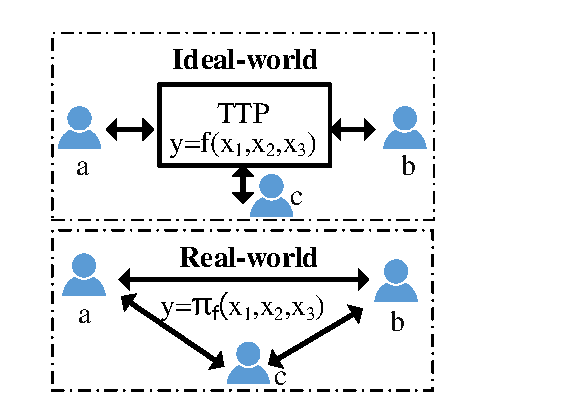
\includegraphics[scale=0.55]{img/ideal-real-v2}
     \caption{Ideal-world vs. real-world}
	\label{fig:ideal-real}
\end{minipage}
%\vspace{-2mm}
\end{figure}
%
%\begin{figure}[t]
%\centering
%\begin{subfigure}{0.5\textwidth}\centering
%\lstset{style=mystyle}
%\begin{lstlisting}[language=C]
%int demo(int a, int b, int c){
%    int r = 1;  int max = a;
%    bool c1 = max < b;
%    if (c1){ max = b; r = 2; }
%    bool c2 = max < c;
%    if (c2){ r = 3; }
%    return r;
%}
%\end{lstlisting}\vspace*{-3mm}
%\caption{The richest one of three millionaires}
%\label{fig:motivation}
%\end{subfigure}
%\quad%\vspace*{-3mm}
%\begin{subfigure}{0.4\textwidth}\centering
%    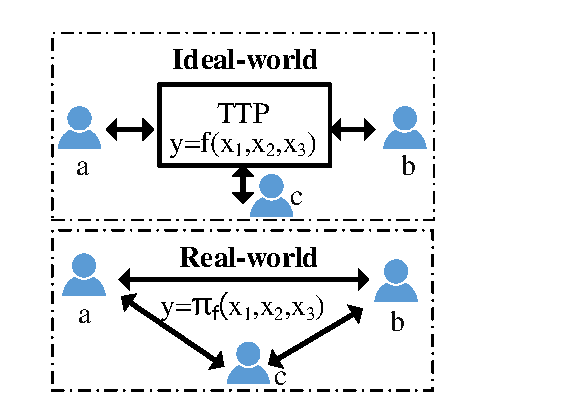
\includegraphics[scale=0.55]{img/ideal-real-v2.pdf}
%    \caption{Ideal-world vs. real-world}
%    \label{fig:ideal-real}
%\end{subfigure}
%\caption{Motivating example}
%\end{figure}

%
%\begin{figure}[t]
%\centering \lstset{style=mystyle}
%\begin{lstlisting}[language=C]
%int demo(int a, int b, int c){
%    int r = 1;  int max = a;
%    bool c1 = max < b;
%    if (c1){ max = b; r = 2; }
%    bool c2 = max < c;
%    if (c2){ r = 3; }
%    return r;
%}
%\end{lstlisting}
%\vspace*{-3mm}
%\caption{The richest one of three millionaires}
%\label{fig:motivation}
%\end{figure}
%
%\begin{figure}[t]
%    \centering
%    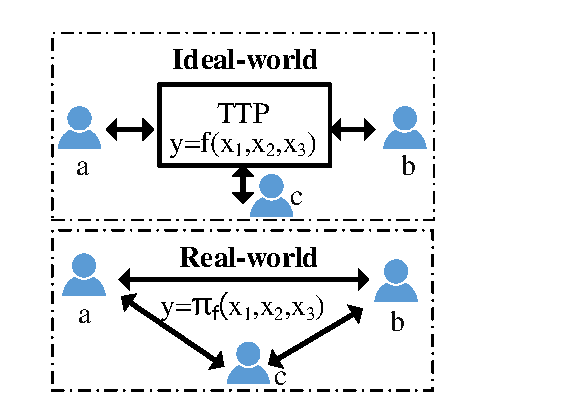
\includegraphics[scale=0.5]{img/ideal-real-v2.pdf}
%    \caption{Ideal-world vs. real-world}
%    \label{fig:ideal-real}
%\end{figure}

Fig.~\ref{fig:motivation} shows a motivating example that computes the richest among three millionaires. %Obviously, whoever executes this program  will know all the inputs   {\tt a}, {\tt b} and {\tt c}.
To preserve the privacy, the millionaires can privately send their inputs to a trusted third party (TTP)
%which computes and sends back the result,
as shown in Fig.~\ref{fig:ideal-real} (ideal-world). This reveals
the richest millionaire with the least leakage of information.
Table~\ref{tab:max3table} shows the leakage  for each result ${\tt r}=1, 2, 3$, as well as the leakage if the secret branching variables {\tt c1} and {\tt c2} are declassified (i.e., from secret to public).

\begin{table}[ht]\vspace{-7mm}
\setlength{\tabcolsep}{4mm}
\centering
\caption{Leakage from each result and declassified secret branching variables}
\label{tab:max3table}
\begin{tabular}{c|c|c|c}
\hline
\textbf{Result}  &  \textbf{Leakage of Result} &\textbf{Leakage of c1} & \textbf{Leakage of  c2} \\ \hline
${\tt r} = 1$   &${\tt a}\geq{\tt b} \wedge {\tt a}\geq{\tt c}$ & ${\tt a}\geq {\tt b}$ & ${\tt a}\geq{\tt c}$    \\ \hline
${\tt r}= 2$    & ${\tt a}<{\tt b} \wedge {\tt b}\geq {\tt c}$ &${\tt a}<{\tt b}$  & ${\tt b}\geq {\tt c}$     \\ \hline
${\tt r}= 3$    &  ${\tt c}>\max({\tt a},{\tt b})$  & ${\tt a}\geq{\tt b}\vee{\tt a}<{\tt b}$ &  ${\tt c}>\max({\tt a},{\tt b})$            \\
\hline
\end{tabular}
\vspace{-4mm}
\end{table}

To achieve the same functionality without TTP, secure multi-party computation (MPC) was proposed~\cite{Yao86,ChaumCD88,GMW,yao82,EvansKR18}. %~\cite{EvansKR18}.
%There are three fundamental MPC protocols: garbled circuits~\cite{yao82,freexor}, secret sharing~\cite{Shamir79,GMW}, and homomorphic encryption~\cite{SHE}.
One can implement the computation using an MPC protocol $\pi$  where
all the parties collaboratively compute the result over their private inputs
%following a MPC protocol
via network communications (shown in Fig.~\ref{fig:ideal-real} (real-world)).
%However, implementing the entire program in an MPC protocol is not efficient in terms of the cost of
%communication and computation.
%Therefore,

To facilitate the application of MPC, MPC frameworks, e.g., Obliv-C~\cite{ZahurE15}, MP-SPDZ~\cite{spdz20} and MPyC~\cite{MPyC20}, are proposed, which provide high-level languages
for %implementing
specifying MPC applications, as well as compilers for translating them into executable implementations.
To improve the performance, such frameworks often allow users to declare secret variables so that only
the values of secret variables are to be protected.
However, in practice, it could be highly non-trivial for non-experts to specify secret variables properly:
declaring too many secret variables degrades the performance while
declaring too less secret variables compromises security.
%As a dishonest party can observe all the intermediate computation results of the program executed by
%the dishonest party.

In this work, we propose an automated synthesis approach %for generating
%security policy which
to declare as few secret variables as possible but without compromising security.
To capture privacy, we formalize the leakage of MPC applications in the ideal-world as a set of %indistinguishable space of
private inputs. For instance, the leakage of the result ${\tt r}=1$ in the motivating example
is the set of inputs %for ${\tt a, b, c}$
such that
${\tt a}\geq{\tt b} \wedge {\tt a}\geq{\tt c}$.
We introduce the notion of security policy, which assigns each variable a security level, to bridge the language-level and protocol-level leakages, so that our approach is independent of specific MPC protocols being used.
The language-level leakage of a security policy is characterized by a set of %indistinguishable space of
private inputs with respect to not only the result but also the values of public variables
in the intermediate computations.
%A security policy should not compromise security, i.e.,
%leak more information as that in the ideal-world.


Based on the leakage characterization, we propose a type system to infer security policies,
inspired by the work for  %that for proving
the noninterference property of programs~\cite{VolpanoIS96}.
Our type system tracks both control-flow and data-flow of information from the private inputs, and infers
a security policy. For instance,
all the variables in the motivating example are inferred as secret.

Though a security policy inferred by the type system formally guarantees that the MPC application will not leak more information than that in the ideal-world, it may be too conservative.
For instance, declassifying the variable {\tt c2} in the example would not compromise security.
As shown in Table~\ref{tab:max3table}, the leakage caused by declassifying {\tt c2} can be deduced from
%is already included in
the leakage of the result. In contrast, we cannot declassify {\tt c1},
as neither ${\tt a}\geq{\tt b}$ nor ${\tt a}<{\tt b}$ can be deduced from the leakage ${\tt c}>\max({\tt a},{\tt b})$.
Once {\tt c1} is declassified, the adversary would learn
if ${\tt a}\geq{\tt b}$ or ${\tt a}<{\tt b}$.
This problem is akin to downgrading and declassification of high security levels in information-flow analysis~\cite{LiZ05}, and could be solved via self-composition~\cite{TerauchiA05,mpcleak18,YangVSGM18}
that often require users to write annotations for procedure contracts and loop invariants.
 %which reduces to the safety problem on two copies of a program
%However, it is still challenging in practice to check safety properties on two copies of a program.
%To address this issue,
In this work, for the sake of efficiency and usability for non-experts,
we propose an alternative approach based on symbolic execution~\cite{King76}.
We leverage a symbolic execution to represent a potentially infinite set of concrete executions and propose an automated approach to infer
if a secret variable can be declassified by reasoning about pairs of symbolic executions.
%\fu{Limiting the reasoning to each pair of symbolic executions could prune away
%irrelevant verification conditions and tightens the search space.}
Our approach can identify that {\tt c2} in the motivating example
can be declassified without compromising security.
The experimental results show that this approach without requiring any annotations for procedure contracts or loop invariants is effective and
the generated security policies can significantly improve
the performance of MPC applications. % when compiled into executable implementations.

%
%Participants can evaluate any function on MPC as long as they agree on it. However, not all functions are privacy-preserving.
%For example, the famous Yao's Millionaires Problem outputs the r of two millionaires without leaking any additional information about their wealth.
%%Each millionaire also knows his wealth.
%With the result of the Millionaires Problem, a millionaire learn the range of another's wealth.
%Such functions leak information from their results.
%Furthermore, a feature of these functions is that they always output symbols or indexes as the results.
%We focus on these kinds of functions and start from an example program in Fig. \ref{max3}.
%
%\lstdefinestyle{mystyle}{
%basicstyle=\ttfamily\footnotesize,
%breakatwhitespace=false,
%breaklines=true,
%captionpos=b,
%keepspaces=true,
%numbersep=5pt,
%showspaces=false,
%showstringspaces=false,
%showtabs=false,
%tabsize=2
%}
%\begin{figure}[ht]
%\centering \lstset{style=mystyle}
%\begin{lstlisting}[language=C]
%obliv char millionaire3(obliv int a, obliv int b, obliv int c){
%    obliv char r = 'a';
%    obliv int max = a;
%    obliv bool c1 = max < b;
%    obliv if (c1){
%        max = b;
%        r = 'b';
%    }
%    obliv bool c2 = max < c;
%    obliv if (c2){
%        r = 'c';
%    }
%    return r;
%}
%\end{lstlisting}
%\caption{The richest one of three millionaires \label{max3}}
%\end{figure}
%
%
%This program outputs who inputs the maximum value.
%It is an extension of Yao's Millionaires Problem.
%The \texttt{obliv \textbf{int}} in Fig. \ref{max3} declares an oblivious integer variable that represents integer typed privacy data.
%\texttt{millionaire3} function contains two if-statements, and applies oblivious control structures.
%The oblivious control structure \texttt{obliv \textbf{if}} makes participants do not know which branch is executed to keep the condition variable privacy.
%\texttt{millionaire3} has three types of output:\texttt{'a'}, \texttt{'b'} and \texttt{'c'}. Participants know the richest millionaire after the execution of the function.
%
%
%Let us reveal some branch conditions to reduce the use of oblivious control structure and analyze the information leak of revealed data.
%An overview of our analysis is in Table \ref{max3table}
%To simplify our discussion, we suppose the three millionaires have different wealth.
%\begin{table}[ht]
%\setlength{\tabcolsep}{1mm}
%\caption{Information leak from results and revealed conditions}
%\label{max3table}
%\begin{tabular}{c|c|c|c}
%\hline
%\textbf{Richest} & \textbf{\begin{tabular}[c]{@{}c@{}}Info learned \\ from c1\end{tabular}} & \textbf{\begin{tabular}[c]{@{}c@{}}Info learned \\ from c2\end{tabular}} & \textbf{\begin{tabular}[c]{@{}c@{}}Info learned \\ from output\end{tabular}} \\ \hline
%A    &
%a $>$ b &
%a $>$ c  &
%\begin{tabular}[c]{@{}c@{}}a $>$ b \\ $\land$ a $>$ c\end{tabular}    \\ \hline
%B      &
%b $>$ a  &
%b $>$ c  &
%\begin{tabular}[c]{@{}c@{}}b $>$ a \\$\land$ b $>$ c\end{tabular}        \\ \hline
%C  &
%\begin{tabular}[c]{@{}c@{}}a $>$ b \\ or b $>$ a\end{tabular}          &
%c $>$ max(a,b)        &
%\begin{tabular}[c]{@{}c@{}}c $>$ a \\$\land$ c $>$ b\end{tabular}         \\ \hline
%\end{tabular}
%\end{table}
%
%Firstly, suppose we only reveal the \texttt{c1}:
%\begin{itemize}
%\item In the case of output \texttt{'a'}, participants know A's wealth is more than B's and C's from the output and learn that A's wealth is more than B's from the revealed data.
%\item In the case of output \texttt{'b'}, participants know B's wealth is more than A's and C's from the output and learn that A's wealth is less than B's from the revealed data.
%\item In the case of output \texttt{'c'}, participants know C's wealth is more than A's and B's from the output and learn who is r in A and B from the revealed data.
%\end{itemize}
%
%In the first two cases,  participants learn nothing useful from the revealed data because they also learn it from the output.
%However, information leak happens because participants cannot know who is r between A and B from the output in the third case.
%Therefore, we cannot reveal \texttt{c1} because it leaks extra information when the execution results \texttt{'c'}.
%
%Then, suppose we only reveal the \texttt{c2}.
%\begin{itemize}
%\item In the case of output \texttt{'a'}, participants learn that A's wealth is more than C's from the revealed data.
%\item In the case of output \texttt{'b'}, participants learn that B's wealth is more than C's from the revealed data.
%\item In the case of output \texttt{'c'}, participants learn C's wealth is more than the r between A and B from the revealed data.
%\end{itemize}
%
%In all cases,  the participants learn nothing useful from the revealed data because they can also learn it from the output.
%There is no information leak when we reveal \texttt{c2}.
%Therefore, we can reveal \texttt{c2} in \texttt{millionaire3} to reduce the use of oblivious control structure without information leak.
%
%For practical programs, determining whether revealing an intermediate private data cause information leak needs experts' knowledge.
%This work aims to propose a method and implement it as an automated verification tool.
%Programmers without expert knowledge can use our tool to appropriately revealing intermediate privacy data without information leak to achieve higher performance.
%
%\subsection{Challenges}
%To achieve our goals, we have to overcome some challenges:
%\begin{enumerate}
%\item How to define and analyze the information leakage of MPC programs with considering revealed result?
%
%Existing work on MPC program's information leakage focuses on the protocol level and ignores the information leakage of the revealed result.
%Our work should define information leakage considering the revealed result at the semantic level.
%To our knowledge, no existing work is the same as ours.
%%We have to design new method and automate it.
%
%\item How to ensure that the program that reveals some intermediate private data does not compromise security?
%
%We allow MPC programs to reveal intermediate privacy data during execution.
%Previous work to allow leakage of intermediate private data does not consider security but trade-off efficiency and security.
%We need to design a method to verify an optimized program's information leakage.
%% \item How to determine our strategy effective and efficient?
%% Unlike other tradeoff work between performance and security, they can reveal any private data of a program to build a test program.
%% Because we aim to hold the program's security, we must ensure an optimized program is secure before regarding it as a study case.
%% We expend much energy to build study cases in the experiment section.
%
%\end{enumerate}

\section{Secure MPC} \label{sec:preli}

%In this section, we briefly recap secure multi-party computation (MPC)

%and three fundamental protocols for implementing MPC applications.
%Their relation is visually shown in Figure~\ref{fig:ideal-real} for 3-party MPC.



%\subsection{Secure Multi-Party Computation}

Fix a set of variables $\Var$ over a domain $\Dom$. We write $\vec{x}_n\in\Var^n$ and $\vec{v}_n\in \Dom^n$ for $x_1, \cdots, x_n$
and $v_1, \cdots, v_n$ respectively.
(The subscript $n$ may be dropped %from $\vec{x}_n$ and $\vec{v}_n$
when it is clear from the context.)
%When we  write $\vec{v}_n\in\Dom^n$ and $\vec{v}_k\in\Dom^k$ for $n\geq k$,
%we mean that $\vec{v}_k$ is a prefix of $\vec{v}_n$.

%We first define secure multi-party computation (MPC) in the ideal world
%and then define MPC in the real world.

\smallskip
\noindent
{\bf MPC in the ideal-world}. An $n$-party MPC application $f:\Dom^n\rightarrow \Rng$ is to confidentially compute a given function $f(\vec{x})$, where each party $\Party{i}$ for $1\leq i\leq n$ sends her
private input $v_i\in \Dom$ to a TTP $\Trust$ which
computes and returns the result $f(\vec{v})$ to all the parties.
In the ideal world, an adversary that controls  any of the $n$ parties
learns no more than the output $f(\vec{v})$ and the private inputs of the corrupted (dishonest) parties.
%and the private inputs controlled by the adversary.

We characterize the leakage of an MPC application $f(\vec{x})$  by
a set of private inputs. %We start by introducing some notations.
In the rest of this paper, we assume, w.l.o.g.,
the first $k$ parties (i.e., $\Party{1},\cdots, \Party{k}$) are corrupted by the adversary for some $k\geq 1$.
%
For a given output $v\in \Rng$, let ${\simeq_v^f}\subseteq \Dom^n$ denote the set
$\{\vec{v}\in \Dom^n\mid f(\vec{v})=v\}$.
Intuitively, ${\simeq_v^f}$ is the set of the private inputs $\vec{v}\in \Dom^n$ under which  $f$ is evaluated to $v$.
From the result $v$, the adversary is able to learn the set ${\simeq_v^f}$, but cannot
%distinguish the private inputs
tell which one from ${\simeq_v^f}$ given $v$. We refer to ${\simeq_v^f}$ as the \emph{indistinguishable space} of the private inputs w.r.t. the result $v$.
The input domain $\Dom^n$ is then partitioned into indistinguishable spaces $\{\simeq_v^f\}_{ v\in \Rng}$.  % i.e.,  $\{\simeq_y^f\mid y\in \Rng\}$,
%and the adversary only learns one set ${\simeq_v^f}$ from the partition $\{\simeq_v^f\}_{ v\in \Rng}$
%for any result $v\in \Rng$.
%

When the adversary controls the parties $\Party{1},\cdots, \Party{k}$,
she will learn the set  $\leak_{\tt iw}^f(v,\vec{v}_k): = \{(v_1,\cdots,v_n)\in\Dom^{n}\mid \vec{v}_k=v_1,\cdots,v_k\}\cap \simeq_v^f$, %\tl{i understand you introduced this before, but here it seems confusing. Shall we change it back?}
%\{(v_1,\cdots,v_k, v'_{k+1}, \cdots, v_n')\mid (v_1,\cdots,v_k, v'_{k+1}, \cdots, v_n') \in {\simeq_v^f}\}$,
from the result $v$ and the adversary-chosen private inputs $\vec{v}_k\in\Dom^k$.
%(Note that the first $k$ values of $\vec{v}_n$ are $\vec{v}_k$).


%
%By slight abuse of notation, we denoted by $(v_1,\cdots, v_n)\simeq_v^f (v_1',\cdots, v_n')$,
%for every $(v_1,\cdots, v_n),(v_1',\cdots, v_n')\in {\simeq_v^f}$.
%The input domain $\Dom^n$ is then partitioned into the indistinguishable spaces $\{\simeq_v^f\}_{ v\in \Rng}$.  % i.e.,  $\{\simeq_y^f\mid y\in \Rng\}$,
%%which is called the \emph{indistinguishable partition} of the input domain $\Dom^n$.
%Therefore, the adversary only learns one indistinguishable space ${\simeq_v^f}$ from the  partition $\{\simeq_v^f\}_{ v\in \Rng}$
%for any public output $v$.
%%
%When the adversary controls the participants $\Party{1},\cdots, \Party{k}$ (i.e.,
%can choose the values of the private inputs $x_1,\cdots,x_k$ for those participants),
%the adversary will learn the indistinguishable space $\{(v_1',\cdots, v_n')\in {\simeq_v^f}\mid v_1'=v_1,\cdots,v_k'=v_k\}$
%from the public output $v$ and the adversary-chosen private inputs $(v_1,\cdots,v_k)$.
%


%Intuitively, if $(x_1,\cdots, x_n),(x_1',\cdots, x_n')\in {\simeq_y^f}$, i.e., $f(x_1,\cdots, x_n)=f(x_1',\cdots, x_n')=y$,
%then $(x_1,\cdots, x_n)$ and $(x_1',\cdots, x_n')$ are equivalent w.r.t. to the computation
%$f(x_1,\cdots, x_n)$.

\begin{definition}[Leakage in the ideal-world]\label{def:leakageinIdeal}
For an MPC application $f(\vec{x}_n)$, the leakage of computing
$v=f(\vec{v}_n)$ in the ideal-world is $\leak_{\tt iw}^f(v,\vec{v}_k)$,
for the adversary-chosen private inputs $\vec{v}_k\in\Dom^k$  and the result $v\in \Rng$.
\end{definition}

%Since the adversary chooses the private inputs $(v_1,\cdots,v_k)$
%for $(x_1,\cdots,x_k)$ and the result $v\in \Rng$ uniquely determines the leakage of computing
%$v=f(v_1,\cdots, v_n)$ for any $v_{k+1},\cdots,v_n$, we denote by $\leak_{\tt iw}(v=f(v_1,\cdots, v_k))$
%the leakage of computing $v=f(v_1,\cdots, v_n)$ in the ideal world for any $v_{k+1},\cdots,v_n$.

\smallskip
\noindent
{\bf MPC in the real-world}.
%Since the presence of a fully trusted third party makes it imaginary in practice,
An MPC application in the real-world is implemented using some MPC protocol $\pi$ (denoted by $\pi_f$)
by which all the parties collaboratively compute $\pi_f(\vec{x})$ over their private inputs
$\vec{v}$ without any TTP $\Trust$. %In general, there are three fundamental protocols to achieve semi-honest security:
%garbled circuits~\cite{yao82,freexor,BeaverMR90}, secret sharing~\cite{Shamir79,GMW}, and homomorphic encryption~\cite{SHE},
%varying in their computational, circuit and communication complexity.
% via network communications,
%where $\pi_f$ denotes the implementation of the computation $f$ using the protocol $\pi$.
A brief introduction of three fundamental protocols can be found in  Appendix~\ref{sec:protocols}.

There are generally two types of adversaries in the real world, i.e., semi-honest and malicious.
An adversary is \emph{semi-honest} (a.k.a.\ passive) if the corrupted parties run the protocol honestly as specified, but may try to learn private information of other parties by observing
the protocol execution (i.e., network messages and program states).
An adversary is \emph{malicious} (a.k.a.\ active) if the corrupted parties
can deviate arbitrarily from the prescribed protocol (e.g., control, manipulate,
and inject messages) in an attempt to learn private information of the other parties.
%
In this work, we consider semi-honest adversaries, which are supported by most MPC frameworks (cf.~\cite{EvansKR18,spdz20})
and %semi-honest
often serve as a basis for MPC in more robust settings with powerful adversaries.
%Recall that secure multi-party computation in real world is implemented using some protocol $\pi$.

A protocol $\pi$ is (semi-honest) secure if what a (semi-honest) adversary can achieve in the real-world can also be achieved by a corresponding adversary in the ideal-world.
Semi-honest security ensures that the corrupted parties learn no more information from executing the protocol than what they can learn from the result and the private inputs of the corrupted parties. Therefore,
the leakage of an MPC application $f(\vec{x})$ in the real-world against
the semi-honest adversary can also be characterized using the
indistinguishability of private inputs.
%Let $\leak_{\tt rw}(v=\pi_f(v_1,\cdots, v_n))\subseteq \Dom^n$ denote the leakage of computing $v=f(v_1,\cdots, v_n)$ in the real-world using
%the protocol $\pi$.


\begin{definition}\label{def:securityinIW}
An MPC protocol $\pi$ is (semi-honest) secure
if for any MPC application $f(\vec{x}_n)$, adversary-chosen private inputs $\vec{v}_k\in\Dom^k$
and result $v\in \Rng$,
the leakage of computing $v=\pi_f(\vec{v}_n)$  is $\leak_{\tt iw}^f(v,\vec{v}_k)$. %=\leak_{\tt rw}(v=\pi_f(v_1,\cdots, v_n)).\]
\end{definition}
%
%\begin{definition}\label{def:securityinIW}
%A protocol $\pi$ is \emph{secure} against a semi-honest adversary,
%if the leakage of computing a MPC application $f(x_1,\cdots, x_n)$ under the protocol
%is the set ${\simeq_y^f}$ for every public output $y=f(x_1,\cdots, x_n)$
%and the adversary only learns the set $\{(x_{i+1},\cdots,x_n) \mid (x_1,\cdots, x_n)\in {\simeq_y^f}\}$ for the adversary-chosen private inputs $(x_1,\cdots,x_i)$.
%\end{definition}

%Formal definitions of semi-honest security refers to~\cite{EvansKR18}.

%
%For the private inputs $x_1,\cdots, x_n, x_1',\cdots, x_n'$,
%we say that $(x_1,\cdots, x_n)$ and  $(x_1',\cdots, x_n')$ are equivalent w.r.t. to
%$f(x_1,\cdots, x_n)$, denoted by $(x_1,\cdots, x_n)\simeq_f (x_1',\cdots, x_n')$,
%if $f(x_1,\cdots, x_n)=f(x_1',\cdots, x_n')$. The subscript $f$ is dropped from the equivalence  relation $\simeq_f$
%when it is clear from the context.
%For every tuple $(x_1,\cdots, x_n)$, we denote by
%$(x_1,\cdots, x_n)_{\simeq}$ the equivalence class of $(x_1,\cdots, x_n)$
%under the equivalence relation $\simeq$.
%We denote by $\mathcal{P}_{\simeq}(D^n)$ the partition
%of $D^n$ induced by the equivalence relation $\simeq$.
%Therefore, for every tuple of private inputs $(x_1,\cdots, x_n)\in D^n$,
%the adversary only learns the equivalence class $(x_1,\cdots, x_n)_{\simeq}$.



\section{Language-level Leakage Characterization}\label{sec:leakagePL}
In this section, we characterize the leakage of MPC applications from the language perspective.

\subsection{A Language for MPC}
%For the sake of presentation,
We consider a simple language {\LANG} for implementing MPC applications.
The syntax of {\LANG} programs is defined as follows. %, which is an extension of the \emph{while} language: % with a declassify operator {\Pdeclassify}.
\begin{align*}
  p  ::=  & {\Pskip} \mid x = e  \mid \ p_1; p_2 \mid   {\Pif} \ x \ {\Pthen} \  p_1 \ {\Pelse} \ p_2 \mid {\Preturn} \ x \\
    & \mid    {\Pwhile} \ x \ \Pdo \ p  \mid {\Prepeat} \ n \ \Pdo \ p
\end{align*}
where $e$ is an expression defined as usual and $n$ is a positive integer.

%and a secure integer type {\Psint}.
Despite its simplicity, {\LANG} suffices to illustrate our approach %describe a wide range of MPC applications
and our tool supports a real-world language. % and fully illustrate our approach.
Note that we introduce two loop constructs.
The {\Pwhile} loop can only be used with the secret-independent conditions
while the {\Prepeat} loop (with a fixed number $n$ of iterations) can have secret-dependent conditions.
%and secret-independent conditional statements.
The restriction of the {\Pwhile} loop
is necessary, as %argued by  Zahur and Evans
the adversary knows when to terminate the loop, so
secret information may be leaked if a secret-dependent condition is used~\cite{ZahurE15}.

The operational semantics of the {\LANG} program is defined in a standard way %using transitions between configurations
(cf.\  Appendix~\ref{sec:semantics}). %, as shown in Figure~\ref{fig:semantics}.
In particular, ${\Prepeat}$ $n$ $\Pdo$ $p$ means repeating the loop body $p$ for a fixed number $n$ times.
A \emph{configuration} is a tuple $\MPCAngle{p, \sigma}$, where $p$ denotes a statement and $\sigma:\Var\rightarrow\Dom$ denotes a state that maps variables to values.
The evaluation of an expression $e$ under a state $\sigma$ is denoted by $\sigma(e)$.
%
A transition from  $\MPCAngle{p, \sigma}$ to $\MPCAngle{p', \sigma'}$
is denoted by $\MPCAngle{p, \sigma}\rightarrow \MPCAngle{p', \sigma'}$ and $\rightarrow^*$ denotes the transitive closure of $\rightarrow$.
%
An \emph{execution} starting from the configuration $\MPCAngle{p, \sigma}$ is a sequence of configurations. We write $\MPCAngle{p, \sigma}\Downarrow \sigma'$
if $\MPCAngle{p, \sigma}\rightarrow^* \MPCAngle{{\Pskip}, \sigma'}$.
We assume that each execution ends in a {\Preturn} statement, i.e.,
all the {\Pwhile}\ loops always terminate.
We denote by $\MPCAngle{p, \sigma}\Downarrow \sigma':v$
the execution returning value $v$.


%%%%%%%%%%%%%%%%%%%%%%%%%%%%%%%%%%%%%%%%%%%%%%%%%%%%%%%%%%%%%%%%%%%%%%%%%%%%%%%%%%%%%

\subsection{Leakage Characterization in Ideal/Real-World}
An MPC application $f(\vec{x})$ is implemented as a {\LANG} program $p$.
An execution of the program $p$ evaluates the computation $f(\vec{x})$
as if a TTP directly executed the program $p$ on the private inputs.
In this setting, the adversary cannot observe any intermediate states of the execution %$\MPCAngle{p, \sigma}\Downarrow \sigma':v$,
other than the final result. % $v$.
%, where the initial state $\sigma$ maps the variables $\vec{x}$ to their private inputs.

Let $\Var^{\tt in}=\{x_1,\cdots,x_n\}\subseteq\Var$ be the set of private input variables.
We denote by $\InitState_0$ %: \Var^{\tt in}\rightarrow \Rng^n$
the set of the initial states.
Given a tuple of values $\vec{v}_k\in\Dom^k$  % for the private input variables $x_1,\cdots, x_k$,
and a result $v\in \Rng$, let $\leak_{\tt iw}^p(v,\vec{v}_k)$ % $\Sigma^p_{v,v_1,\cdots,v_k}$
denote the set of states $\sigma\in \InitState_0$ such that
$\MPCAngle{p, \sigma}\Downarrow \sigma':v$ for some state $\sigma'$ and $\sigma(x_i)=v_i$ for $1\leq i\leq k$.
Intuitively, when the adversary controls the parties $\Party{1},\cdots, \Party{k}$,
she learns the set of states $\leak_{\tt iw}^p(v,\vec{v}_k)$
from the result $v$ and the adversary-chosen private inputs $\vec{v}_k\in\Dom^k$.
%
%\tl{not quite understand this} For the adversary-chosen values $(v_1,\cdots, v_k)\in\Dom^k$ for the private inputs $x_1,\cdots, x_k$,
%the adversary cannot distinguish the initial states $\sigma\in\leak_{\tt iw}^p(v,v_1,\cdots,v_k)$ from the result $v$ in the ideal-world. %Therefore, $\leak_{\tt iw}^{v,v_1,\cdots,v_k}$ is the set of indistinguishable initial states to the adversary
%from the execution $\MPCAngle{p, \sigma}\Downarrow \sigma':v$  for any $\sigma\in \leak_{\tt iw}^{v,v_1,\cdots,v_k}$.
%We denote $\leak(\MPCAngle{p, \{x_1\mapsto v_1,\cdots,x_n\mapsto v_n\}}\Downarrow \sigma':v)$ the set of indistinguishable states $\Sigma^p_v(v_1,\cdots,v_k)$.
% and $\Sigma^f_v\subseteq \Sigma^f$ for a given value $v\in \Rng$ denote the set of initial states $\sigma$
%such that $\MPCAngle{p, \sigma}\Downarrow \sigma':v$ for some state $\sigma'$.
%For a given tuple of values $(v_1,\cdots,v_k)$ for the private inputs $(x_1,\cdots,x_k)$, let $\Sigma^f_v(v_1,\cdots,v_k)$ be the set
%of initial states $\sigma$ such that $\sigma\in\Sigma^f_v$
%and $\sigma(x_i)=v_i$ for all $1\leq i\leq k$.
We can reformulate the leakage of an MPC application $f(\vec{x})$ in the ideal-world (cf.\ Definition~\ref{def:leakageinIdeal})
as follows:


\begin{proposition}
Given an MPC application $f(\vec{x}_n)$  implemented by a program $p$,
$\vec{v}_n'\in\leak_{\tt iw}^f(v,\vec{v}_k)$
iff there exists a state $\sigma\in \leak_{\tt iw}^p(v,\vec{v}_k)$
such that $\sigma(x_i)=v_i'$ for $1\leq i\leq n$.
%
%the \emph{leakage} to the adversary of an execution $\MPCAngle{p, \sigma}\Downarrow \sigma':v$ from an initial state
%$\sigma\in \Sigma^f_v(v_1,\cdots,v_k)$ is the set of indistinguishable states $\Sigma^f_v(v_1,\cdots,v_k)$, where the values $(v_1,\cdots, v_k)\in\Dom^k$ of the private inputs $x_1,\cdots, x_k$ are chosen by the adversary.
\end{proposition}



%
%\begin{figure}[ht]
%    \centering
%  \begin{align*}
%%&  &  T::= & {\Pint} \mid {\Psint} \\
%&  &  p::= & {\Pskip} \mid x = e  \mid \ p_1; p_2 % \\ %\mid T\ x = {\Pdeclassify}(y)  \\ \mid  x = {\Pdeclassify}(e)
% \mid   {\Pif} \ x \ {\Pthen} \  p_1 \ {\Pelse} \ p_2 \mid {\Pwhile} \ x \ \Pdo \ p \mid {\Preturn} \ x
%    \end{align*}
%%    \vspace*{-4mm}
%    \caption{Syntax of {\LANG}}
%    \label{fig:syntax}
%\end{figure}

%
%\begin{figure}[ht]
%    \centering\footnotesize
%    \begin{tabular}{cc}
%%%%%%%%%%%%%%%%%%%%%%%%%%%%%%%%%%%%%%%%%%%
%    $\begin{array}{c}
%        \MPCState{e}{\sigma}=v \\
%        \hline
%        \MPCAngle{x=e, \sigma} \rightarrow_{\obv{\epsilon}} \MPCAngle{{\Pskip}, \sigma[x\mapsto v]}
%    \end{array}$ &
%%%%%%%%%%%%%%%%%%%%%%%%%%%%%%%%%%%%%%%%%%%
%   %    $\begin{array}{c}
%%        \MPCState{e}{\sigma}=v \\
%%        \hline
%%        \MPCAngle{T \ x = e, \sigma} \rightarrow_{\obv{\epsilon}}  \MPCAngle{{\Pskip}, \sigma[x\mapsto v]}
%%    \end{array}$ \\ \\
%%%%%%%%%%%%%%%%%%%%%%%%%%%%%%%%%%%%%%%%%%%
%       $\begin{array}{c}
%        \MPCState{y}{\sigma}=v \\
%        \hline
%        \MPCAngle{x = {\Pdeclassify}(y)} \rightarrow_{\obv{v}}  \MPCAngle{{\Pskip}, \sigma}
%    \end{array}$    \\ \\
%%%%%%%%%%%%%%%%%%%%%%%%%%%%%%%%%%%%%%%%%%%
%   $\begin{array}{c}
%        \MPCAngle{p_{1}, \sigma_{1}}             \rightarrow_{\obv{o_1}}      \MPCAngle{ {\Pskip}, \sigma_{2} } \quad
%        \MPCAngle{p_{2}, \sigma_{2}}    \rightarrow_{\obv{o_2}}   \MPCAngle{ p_{2}' , \sigma_{3} } \\
%        \hline
%        \MPCAngle{p_{1};p_{2}, \sigma_{1}}       \rightarrow_{\obv{o_1\cdot o_2}}     \MPCAngle{p_{2}', \sigma_{3}}
%    \end{array}$ &
%%%%%%%%%%%%%%%%%%%%%%%%%%%%%%%%%%%%%%%%%%%
%    $\begin{array}{c}
%        \MPCAngle{p_1,\sigma_{1}}    \rightarrow_{\obv{o}}    \MPCAngle{ p_1', \sigma_{2}}    \quad     p_{1}' \neq {\Pskip} \\
%        \hline
%        \MPCAngle{p_{1} ; p_{2}, \sigma_{1}} \rightarrow_{\obv{o}}  \MPCAngle{p_1^{\prime};p_2, \sigma_{2}}
%    \end{array}$  \\ \\
%%%%%%%%%%%%%%%%%%%%%%%%%%%%%%%%%%%%%%%%%%%
% $\begin{array}{c}
%        p= \MPCState{e}{\sigma} \ ? \ p_1 : \ p_2 \\
%        \hline
%        \MPCAngle{{\Pif} \ e \ {\Pthen} \  p_1 \ {\Pelse} \ p_2, \sigma}   \rightarrow_{\obv{\MPCState{e}{\sigma}}}   \MPCAngle{p,\sigma}
%    \end{array} $ &
%%%%%%%%%%%%%%%%%%%%%%%%%%%%%%%%%%%%%%%%%%%
%   $ \begin{array}{c}
%        p'=\MPCState{e}{\sigma} \ ? \ p;\text{while } e \text{ do } p \ : \ {\Pskip} \\
%        \hline
%        \MPCAngle{{\Pwhile} \ e \ \Pdo \ p, \sigma}\rightarrow_{\obv{\MPCState{e}{\sigma}}}  \MPCAngle{p',\sigma}
%    \end{array}$  \\ \\
%            $\begin{array}{c}
%        \MPCState{x}{\sigma}=v \\
%        \hline
%        \MPCAngle{{\Preturn} \ x)} \rightarrow_{\obv{v}} \MPCAngle{{\Pskip}, \sigma}
%    \end{array}$    &
%%%%%%%%%%%%%%%%%%%%%%%%%%%%%%%%%%%%%%%%%%%    \\
%    \end{tabular}
%    \caption{Semantics of {\LANG}}
%    \label{fig:semantics}
%    % instrumented semantics
%\end{figure}
%
%We first define the sequential semantics of {\LANG}  which is used to evaluate a secure multi-party computation $f$
%as if a trust-third-party (TTP) directly computes $f$ over the input data.
%The ideal-world semantics is defined using transitions between configurations, as shown in Figure~\ref{fig:semantics}.
%A configuration is a tuple $\MPCAngle{p, \sigma}$, where $p$ denotes a statement and $\sigma$ denotes a state that maps from variables to values.
%The evaluation of an expression $e$ under a state $\sigma$ is denoted by $\MPCState{e}{\sigma}$.
%A transition from a configuration $\MPCAngle{p, \sigma}$ to a configuration $\MPCAngle{p', \sigma'}$
%is denoted by $\MPCAngle{p, \sigma}\rightarrow_{\obv{o}} \MPCAngle{p', \sigma'}$, where $\obv{o}$ denotes the observation of the transition.
%We denote by $\rightarrow^*$ the transitive closure of $\rightarrow$, where observation is concatenated into an
%observation traces. An execution starting from a configuration $\MPCAngle{p, \sigma}$ ends in the state
%$\sigma'$ with observation trace $\obv{o}$ is written as $\MPCAngle{p, \sigma}\Downarrow_{\obv{o}} \sigma'$,
%if $\MPCAngle{p, \sigma}\rightarrow_{\obv{o}} \MPCAngle{{\Pskip}, \sigma'}$.


%\subsection{Leakage Characterization in Real-World}
We use security policies to characterize the leakage of MPC applications in the real-world.
%instead of modeling concrete MPC protocols,

%to characterize leakage of MPC applications in the real-world.


%\smallskip
\noindent{\bf Security level.}
%To define security policies,
We consider a lattice of security levels $\seclev=\{\Sec,\Pub\}$
with $\Pub \sqsubseteq\Pub$, $\Pub \sqsubseteq\Sec$, $\Sec \sqsubseteq\Sec$
and $\Sec \not\sqsubseteq\Pub$.
We denote by $\ell_1\sqcup\ell_2$ the least upper bound of
two security levels $\ell_1,\ell_2\in\seclev$, namely,
$\ell\sqcup \Sec = \Sec\sqcup \ell=\Sec$ for $\ell\in\seclev$
and $\Pub\sqcup \Pub=\Pub$.


%\smallskip
%\noindent{\bf Security policy.}
%Fix an MPC application $f(\vec{x}_n)$ whose
%functionality is implemented by a program $p$.


\begin{definition}
A \emph{security policy} $\varrho:\Var\rightarrow \seclev$ for the MPC application $f(\vec{x})$ is a function that associates each variable $x\in \Var$ with a security level $\ell\in \seclev$.
\end{definition}

Given a security policy $\varrho$ and a security level $\ell\in \seclev$,
let $\Var^\ell:=\{x\mid \varrho(x)=\ell\}\subseteq \Var$, i.e., the set of
variables with the security level $\ell$ under $\varrho$.
We lift the order $\sqsubseteq$ to security policies, namely, $\varrho\sqsubseteq\varrho'$  if $\varrho(x)\sqsubseteq\varrho'(x)$ for each $x\in \Var$.
%
When executing the program $p$ with a security policy $\varrho$ using an MPC protocol $\pi$, we assume that
the adversary can observe the values of the public variables $x\in \Var^{\Pub}$,
but not that of the secret variables $x\in \Var^{\Sec}$. This is a practical assumption and can be  well-supported by the existing approach.
For instance, Obliv-C~\cite{ZahurE15} allows developers to define an MPC application in an extension of C language, when compiled and linked, the result will be a concrete garbled circuit protocol $\pi_p$ whose computation does not reveal the values of any oblivious-qualified variables.
Thus, all the secret variables specified by the security policy $\varrho$ can be declared as oblivious-qualified variables in Obliv-C,
while all the public variables specified by the security policy $\varrho$ are declared without oblivious-qualification.
Similarly,
MPyC~\cite{MPyC20} is a Python package for implementing MPC applications that allows programmers to define instances of secret-typed variable classes using Python's class mechanism.
When executing MPC applications, instances of secret-typed class variables are protected via Shamir's secret sharing protocol~\cite{Shamir79}.
Thus, all the secret variables specified by the security policy $\varrho$ can be declared as instances of secret-typed variable classes in MPyC,
while all the public variables specified by the security policy $\varrho$ are declared as instances of Python's standard classes.
%We assume that the underlying MPC protocol $\pi$ is secure, namely,
%for every IFP $\varrho:\Var\rightarrow \seclev$,
%the adversary cannot observe the values of secret variables $x\in \Var^{\Sec}$,
%but can observe the values of public variables $x\in \Var^{\Pub}$
%when executing the program $p$ under the protocol $\pi$.
%%
%We argue that this assumption is feasible. \tl{what is the logic link here?}
%For instance, Obliv-C allows developers to define a SPMC application in an extension of C language, when compiled and linked,
%the result will be a concrete garbled circuit protocol $\pi_p$ whose computation does not reveal
%the values of any oblivious-qualified variables~\cite{ZahurE15}.
%Thus, all the variables associated with $\Sec$ in the IFP $\varrho$ can be declared as oblivious-qualified variables in Obliv-C,
%while all the variables associated with $\Pub$ in the IFP $\varrho$ are declared without oblivious-qualification.
%\fu{Add more examples.}


\smallskip
\noindent{\bf Leakage under a security policy.}
Fix a security policy $\varrho$ for the program $p$. Remark that the values of the secret variables will not be known even at runtime for each party, as they are encrypted.
This means that, unlike the secret-independent conditions, the secret-dependent conditions cannot be executed normally, and thus should be removed using, e.g., multiplexers, before transforming into circuits.
%In contrast, the truth value of each secret-independent conditions will be known at runtime for each party
%so that the circuit of branches are to be generated at runtime. %instead of the whole conditional statement.
%Therefore, to define the leakage of the program $p$ under the policy $\varrho$, we first have
%to remove secret-dependent conditions.
%Furthermore, while loops should also be unfolded.
%We denote by ${\sf unfold}(p)$ the program $p$ after loop unfolding.
%Note that in this work we only consider bounded loops, i.e., each loop is bounded
%by a public constant otherwise the loop condition will leak.
%These statements are removed by
%Formally,
We define the transformation $\Enc_\varrho(\cdot,\cdot)$, where $c$ is the selector of a multiplexer.
%which is recursively defined as follows:
{\small\begin{align*}
   &  \Enc_\varrho(c,p_1; p_2)\triangleq\Enc_\varrho(c,p_1);\Enc_\varrho(c,p_2) \qquad\qquad \quad\quad~~ \Enc_\varrho(c,{\Preturn} \ x)\triangleq {\Preturn} \ x \\
%%%%%%%%%%%%%%%%%%%%%%%%%%%%
%   & \Enc_\varrho(c,x = e)\triangleq
%            \left\{
%              \begin{array}{ll}
%                 x=e, & \hbox{if $c=1$;} \\
%                x= x+ c\times (e-x), & \hbox{otherwise.}
%              \end{array}
%            \right.\\
   & \Enc_\varrho(c,x = e)\triangleq x= x+ c\times (e-x)  \qquad \qquad \qquad\Enc_\varrho(c,\Pskip)\triangleq \Pskip  \\
%%%%%%%%%%%%%%%%%%%%%%%%%%%%
  & \Enc_\varrho(c,{\Pif} \ x \ {\Pthen} \  p_1 \ {\Pelse} \ p_2 )\triangleq
\left\{
  \begin{array}{ll}
    {\Pif} \ x \ {\Pthen} \  \Enc_\varrho(1,p_1) \ {\Pelse} \ \Enc_\varrho(1,p_2), & \hbox{if $c=1\wedge\varrho(x)=\Pub$;} \\
   \Enc_\varrho(c\& x, p_1);\Enc_\varrho(c\& \neg x, p_2), & \hbox{otherwise.}
  \end{array}
\right. \\
%%%%%%%%%%%%%%%%%%%%
  & \Enc_\varrho(c,{\Pwhile} \ x \ \Pdo\ p)\triangleq
            \left\{
              \begin{array}{ll}
               {\Pwhile} \ x \ \Pdo\ \Enc_\varrho(1,p), & \hbox{if $c=1\wedge\varrho(x)=\Pub$;} \\
               \textcolor{red}{\tt Error}, & \hbox{otherwise.}
              \end{array}
            \right. \\
&   \Enc_\varrho(c,{\Prepeat} \ n \ \Pdo\ p)\triangleq {\Prepeat} \ n \ \Pdo\ \Enc_\varrho(c,p)
\end{align*}}
%\tl{it seems that $\Enc_\varrho(c,x = e)$ does not need case distinction?}
Intuitively, %$\Enc(c,{\Pif} \ x \ {\Pthen} \  p_1 \ {\Pelse} \ p_2 )$ removes the
%secret-dependent conditional statement while preserves the conditional semantics.
%Our transformation $\Enc_\varrho(\cdot,\cdot)$ takes into account both control-flow and data-flow of information from private inputs.
$\Enc(c,x = e)$ simulates a multiplexer with two different values
depending on whether the assignment $x = e$ is in the scope of some secret-dependent conditions.
At runtime, the value $e$ is assigned to $x$ if $c$ is $1$, otherwise $x$ does not change.
$\Enc_\varrho(c,{\Pwhile} \ x \ \Pdo\ p)$ enforces that the {\Pwhile}\ loop is used in secret-independent conditions
and $x$ is public in the security policy $\varrho$ otherwise throws an error.
The other cases are trivial.
We denote by $\widehat{p}_\varrho$ the program $\Enc_\varrho(1,p)$ on which
we will define the leakage of $p$ in the real-world.
%To make intermediate computation results explicit, we assume that $p_\varrho$



For every state $\sigma: \Var\rightarrow \Rng$,
let $\sigma^{\Pub}:\Var^{\Pub}\rightarrow\Rng$ denote the
state that is the projection of the state $\sigma$ onto the public variables $\Var^{\Pub}$.
For each execution $\MPCAngle{\widehat{p}_\varrho, \sigma_1}\Downarrow \sigma_2$,  we denote
by $\MPCAngle{\widehat{p}_\varrho,\sigma_1}\Downarrow_\varrho^{\Pub} \sigma_2$ the sequence
of configurations where each state $\sigma$ %in the execution $\MPCAngle{\widehat{p}_\varrho, \sigma_1}\Downarrow \sigma_2$
is replaced by the state $\sigma^{\Pub}$.

Recall that the adversary can observe the values of public variables $x\in \Var^{\Pub}$
when executing the program $\widehat{p}_\varrho$. %  under the protocol $\pi$.
Thus, from an execution $\MPCAngle{\widehat{p}_\varrho,\sigma_1}\Downarrow\sigma_2:v$,
she can observe the sequence $\MPCAngle{\widehat{p}_\varrho,\sigma_1}\Downarrow_\varrho^{\Pub} \sigma_2$ and the result $v$, written as $\MPCAngle{\widehat{p}_\varrho,\sigma_1}\Downarrow_\varrho^{\Pub} \sigma_2:v$.
%
%Suppose the adversary chooses the values $(v_1,\cdots, v_k)\in\Dom^k$ for the private inputs $x_1,\cdots, x_k$
%and $\sigma_1\in\Sigma^p_v(v_1,\cdots,v_k)$,
%
For every state $\sigma\in\leak_{\tt iw}^p(v,\vec{v}_k)$,
we denote by $\leak_{\tt rw}^{p,\varrho}(v,\sigma)$
the set of states $\sigma'\in\leak_{\tt iw}^p(v,\vec{v}_k)$ such that
$\MPCAngle{\widehat{p}_\varrho,\sigma'}\Downarrow_\varrho^{\Pub} \sigma_1':v$
and $\MPCAngle{\widehat{p}_\varrho,\sigma}\Downarrow_\varrho^{\Pub} \sigma_1:v$ are identical.
%Given the adversary-chosen values $(v_1,\cdots, v_k)\in\Dom^k$ for the private inputs $x_1,\cdots, x_k$,
%let $\Sigma^{p,\varrho}_{\sigma,v_1,\cdots, v_k}$ be the set of initial states
%$\sigma'\in \Sigma^{p,\varrho}_{\sigma}$ such that $\sigma'(x_i)=v_i$ for $1\leq i\leq k$.



%
%
%Thus, observing the values of the public variables $\Var_\varrho^{\tt pub}$ in the intermediate computations of
%an execution $\MPCAngle{p, \sigma}\Downarrow \sigma'$ from an initial state
%$\sigma\in \Sigma^f$ is the same as observing the values of the public variables in the final
%state $\sigma'$. For a given state $\sigma$ and IFP $\varrho$, we denote by $\sigma_{\downharpoonright_{\varrho}^{\tt pub}}$
%the projection of the state $\sigma$ onto the public variables $\Var_\varrho^{\tt pub}$ defined in the IFP $\varrho$.
%For any valuation of the public variables $\beta:\Var_\varrho^{\tt pub}\rightarrow\Rng$,
%let $\Sigma^f_\beta\subseteq \Sigma^f$ denote the set of initial states
%$\sigma$ such that $\MPCAngle{p, \sigma}\Downarrow \sigma'$ and $\sigma'_{\downharpoonright_{\varrho}^{\tt pub}}=\beta$.
%Thus, observing the values of public variables in $\beta$ only reveals
%the set $\Sigma^f_\beta$.


\begin{definition}
A security policy $\varrho$ is \emph{perfect} for a given MPC application $f(\vec{x}_n)$ implemented by the program $p$, denoted by $\varrho\models_p f(\vec{x}_n)$,
if $\Enc_\varrho(1,p)$ does not throw any errors, and for adversary-chosen private inputs $\vec{v}_k\in\Dom^k$, the result $v\in\Rng$,
and the state $\sigma\in\leak_{\tt iw}^p(v,\vec{v}_k)$,
we have  that \[\leak_{\tt iw}^p(v,\vec{v}_k)=\leak_{\tt rw}^{p,\varrho}(v,\sigma).\]
%
%and for every initial state $\sigma\in \Sigma^f$,
%the \emph{leakage} of an execution $\MPCAngle{p, \sigma}\Downarrow \sigma'$ under the protocol $\pi$
%is the set of initial states $\Sigma^f_\beta$, where $\beta=\sigma'_{\downharpoonright_{\varrho}^{\tt pub}}$.
\end{definition}
%
Intuitively, a perfect security policy $\varrho$ ensures that
for every state $\sigma\in\leak_{\tt iw}^p(v,\vec{v}_k)$,
from the observation $\MPCAngle{\widehat{p}_\varrho,\sigma}\Downarrow_\varrho^{\Pub} \sigma':v$,
%of the execution $\MPCAngle{\widehat{p}_\varrho,\sigma_1}\Downarrow\sigma_2:v$,
the adversary only learns the same set
$\leak_{\tt iw}^p(v,\vec{v}_k)$ of initial states as that in the ideal-world.

Our goal is to compute a perfect security policy $\varrho$ for every program $p$ that implements
the MPC $f(\vec{x})$. A naive way %to compute a perfect policy $\varrho$
is to assign the high security level
$\Sec$ to all the variables $\Var$, which  %which definitively guarantees $\varrho\models_p f(\vec{x})$.
%However, this policy $\varrho$
may however suffer from a lower performance,
as all the intermediate computations have to be performed on encrypted data
and conditional statements have to removed.
Ideally, a security policy $\varrho$ should not only be perfect but also annotate as few secret variables as possible.


\begin{comment}
\subsection{Secure multi-party computation}

A secure multi-party computation is given by a function $f(x_1,\cdots, x_n)$ whose
function body is a statement $p$ in {\LANG}.


The goal of Secure Multi-party computation (MPC) is to enable a group of $n$ participants who do not trust each other or any third party to jointly compute a function $f(x_1,\cdots,x_n)$
where the $i$-th participant owns the private input $x_i$.
MPC ensures the computation process reveals nothing but the result of $f$ to participants.

Yao firstly introduced the MPC problem in the early 1980s \cite{EvansKR18}.
In \cite{yao82}, Yao proposed Yao's garbled circuit protocol for solving the MPC problem.
Goldreich et al. \cite{GMW} proposed an additive secret sharing approach to solve MPC.
A decade ago, Damg{\aa}rd et al. \cite{SHE} proposed a new MPC approach based on %a somewhat
homomorphic cryptosystems.
The above three protocols and their ideas became the basis of research work in the field of MPC protocol design.
Garbled circuits, secret sharing, and homomorphic encryption have become the base protocols for today's MPC implementations.
Due to the unresolved performance issues of homomorphic encryption, real-world MPC implementations tend to choose either garbled circuit-based protocols or secret-sharing-based protocols.
In the experiment section, we consider experiments on the implementation of these two protocols.

\subsection{Adversary and security model}
\subsubsection{Adversary model}
We consider a passive adversary who %A passive adversary are curious but honest attackers, also known as semi-honest adversary. A passive adversary
will execute the protocol honestly, but may try to get as much information as possible from the messages received by the other participants.
This means that a passive adversary can only try to get secret information by observing their own view during the execution of the protocol. % and cannot take any other attack action.

The adversary in MPC is also a participant in the computation.
We consider multiple colluding adversaries as an adversary who corrupts multiple participants.

% Another class of adversaries is the active adversary, also called malicious adversary.
% The active adversary can make the corrupted participants deviate from the protocol rules to execute the protocol at will.
% A active adversary has the same ability to analyze the protocol execution process as a passive adversary,
% but a malicious adversary can take arbitrary attack actions during the protocol execution, such as controlling the network and interrupting the protocol execution.

\subsubsection{Security model}
MPC security is described in a real-ideal paradigm.
Real-ideal paradigm introduces a well-defined ideal world that covers all security requirements, and defines security by discussing the relationship between the real world and the ideal world.
The Figure \ref{fig:real-ideal} explains the difference between the real world and the ideal world.

\begin{figure}[h]
    \centering
    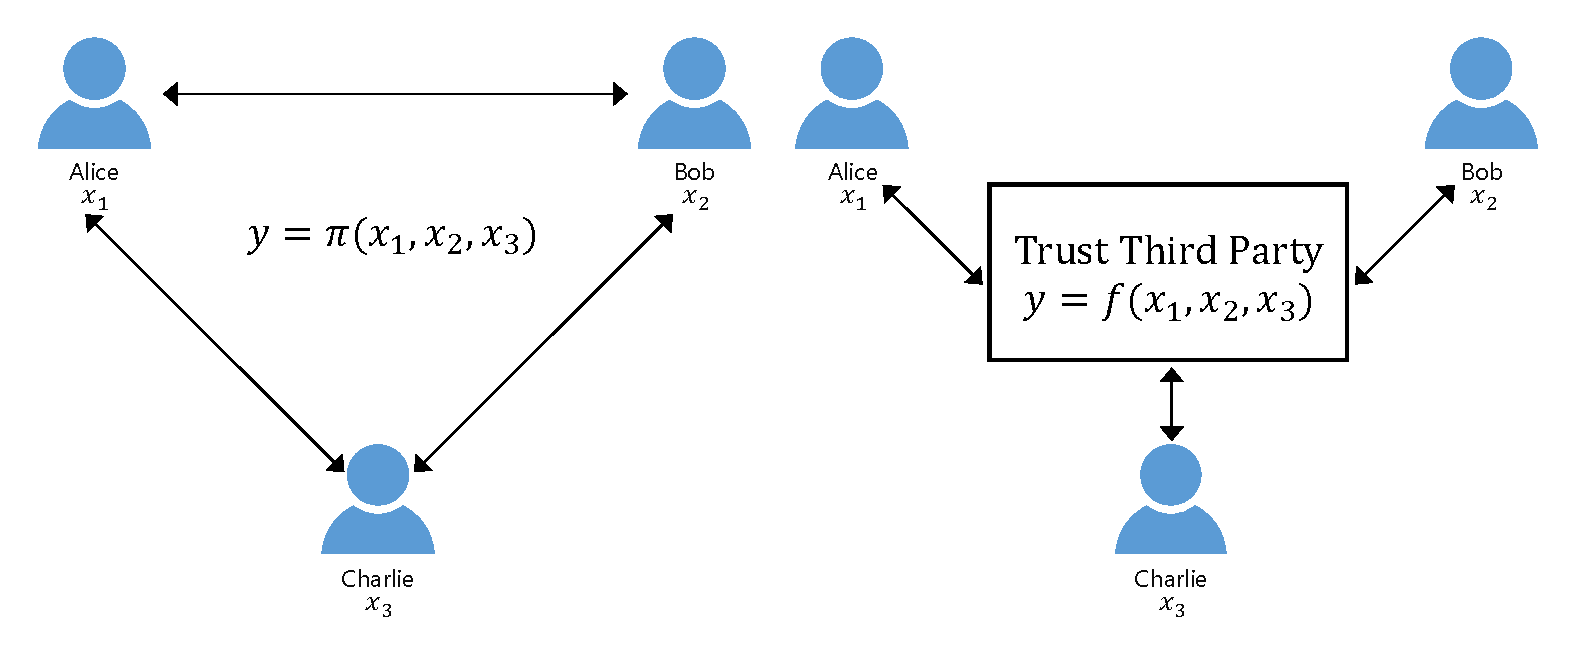
\includegraphics[scale=0.33]{img/real-ideal.pdf}
    \caption{Real-world vs. Ideal-world}
    \label{fig:real-ideal}
\end{figure}



In the real world, all participants communicate with each other through the protocol $\pi$.
Participant $P_i$ generates the message to be sent in the next communication round through the rules of the protocol $\pi$.
% based on the security parameters, random tape, private input $x_i$ and all messages received so far .
At the end of the protocol execution, participants will give output according to the rules of the protocol.

In the ideal world, each participant $P_i$ secretly sends its private input $x_i$ to a TTP %fully trusted third party $\mathcal{T}$.
The $\mathcal{T}$ securely compute $y=f(x_1,...,x_n)$ and returns the result to all participants.


The view of participant $P_i$ consists of its private input $x_i$, random tape, and all messages received during the protocol execution.
An adverasry's view consists of views of all corrupt parties.
The ideal world uses an simulator \textit{Sim} to simulate the participant $P_i$'s view.
The \textit{Sim} receives private input $x_i$ and the result, output the view of each $P_i$.
If the views of the adversary in the real world is indistinguishable from the views of adversary in the ideal world,
then the protocol $\pi$ is secure under the attack of a passive adversary.


The attack action of a passive adversary is to output its entire view.

Let $\pi$ be the MPC protocol evaluating the function $f$, $k$ be the security parameter, $\mathcal{C}$ be the set of corrupted participants, %of the adversary,
and $V_i$ (resp. $\textit{Sim}(x_i, y)$) be the view of the participant $P_i$ in the real (resp. ideal) world.
We define the probability distribution \tl{??} of the following two random variables:
\begin{itemize}
    \item $\text{Real}_{\pi}(k, \mathcal{C};x_1,\cdots,x_n):$ Participants execute protocol $\pi$  with the security parameter $k$ honestly over their private inputs $x_1,\cdots,x_n$. \\
    Outputs $\{V_i\mid  i\in \mathcal{C}\}$.
    \item $\text{Ideal}_{f,\textit{Sim}}(k, \mathcal{C};x_1,\cdots ,x_n):$ The trust party computes $y=f(x_1,\cdots,x_n)$.\\
    Outputs $\{\textit{Sim}(x_i,y)\mid i\in \mathcal{C}\}$.
\end{itemize}

\begin{definition}[Passive security]
    A protocol $\pi$ securely implements the function $f$ in the presence of a passive adversary if there exists a simulator \textit{Sim}
    such that, for all subsets of the corrupted participants set $\mathcal{C}$, the probability distributions
    \[\text{Real}_{\pi}(k, \mathcal{C};x_1,\cdots,x_n) \]
    and
    \[\text{Ideal}_{f,\textit{Sim}}(k, \mathcal{C};x_1,\cdots,x_n)\]
    are indistinguishable (in $k$) \tl{needs to be defined?} for all inputs $x_1,\cdots,x_n$.
\end{definition}


%%%%%%%%%%%%%%%%%%%%%%%%%%%%%%%%%%%%%%%%%%%%%%%%%%%%%%%%%%%%%%%%%%%%%%%%%%%%%%%%%%%%%%%%%%%%%%%%%%%%%%%%%%%%%



%\subsubsection{Privacy type system}
%Figure \ref{type} shows the type system of public and secret variables. $\mathbb{P}$ denotes public type and $\mathbb{S}$ denotes secret type.
%Oblivious RAM (ORAM) \cite{ORAM} is a memory abstraction that allows arbitrary memory access without leaking any information about which locations are accessed.
%MPC programs can access an array item by secret index using ORAM without leaking the index value.
%
%Our privacy type system statically assigns privacy type to variables.
%The privacy environment $\Gamma:V \rightarrow \mathcal{L}$ is a mapping from variable to privacy types where $V$ is the set of variables and $\mathcal{L}=\{\mathbb{P},\mathbb{S}\}$ with $\mathbb{P}\sqsubseteq \mathbb{S}$.
%We  summarize several rules of the privacy type system in Figure \ref{type}:
%\begin{enumerate}
%    \item Public variables can be assigned to secret variables, but not vice versa.
%    \item \textit{reveal} operator convert secret variables to public variables.
%    \item Secret variable can be as the index of ORAM array.
%    \item The control flow of while-statement and if-statement depends on public variables while Obliv if-statement use secret variables as control flow condition.
%\end{enumerate}
%To avoid the occurrence of side-channel, we assume that the statements in the oblivious control structure can read but not write to outer scope public variable.
%
%\begin{figure}[ht]
%    \centering
%    \label{type}
%    \[
%    \begin{array}{cc}
%        \text{Sequence} \\
%        \Gamma \vdash p_1 \quad \Gamma \vdash p_2 \\
%        \hline
%        {\Gamma \vdash p_1;p_2  }
%    \end{array}
%    \quad
%    \begin{array}{c}
%        \text{While} \\
%        \Gamma \vdash e : \mathbb{P} \quad \Gamma \vdash p \\
%        \hline
%        {\Gamma \vdash \text{while } e \text{ do } p }
%    \end{array}
%    \]
%    \[
%    \begin{array}{c}
%        \text{If} \\
%        \Gamma \vdash e : \mathbb{P} \quad \Gamma \vdash p_1 \quad \Gamma \vdash p_2 \\
%        \hline
%        {\Gamma \vdash \text{if } e \text{ then } p_1 \text{ else } p_2 }
%    \end{array}
%    \]
%    \[
%    \begin{array}{c}
%        \text{Obliv If} \\
%        \Gamma \vdash e : \mathbb{S} \quad \Gamma \vdash p_1 \quad \Gamma \vdash p_2 \\
%        \hline
%        {\Gamma \vdash \text{Obliv if } e \text{ then } p_1 \text{ else } p_2 }
%    \end{array}
%    \]
%    \[
%    \begin{array}{c}
%        \text{BinOp} \\
%        \Gamma \vdash e_1: \tau_1 \quad \Gamma \vdash e_2: \tau_2 \quad \tau_2 \sqsubseteq \tau_1\\
%        \hline
%        {\Gamma \vdash e_1 \text{ op } e_2: \tau_1  }
%    \end{array}
%    \]
%    \[
%    \begin{array}{c}
%        \text{\small{Neg}} \\
%        \Gamma \vdash e: \tau \\
%        \hline
%        {\Gamma \vdash \neg e: \tau  }
%    \end{array}
%    \quad
%    \begin{array}{c}
%        \text{\small{Reveal}} \\
%        \Gamma \vdash e: \mathbb{S} \\
%        \hline
%        {\Gamma \vdash \textit{reveal } e: \mathbb{P}  }
%    \end{array}
%    \]
%    \[
%    \begin{array}{c}
%            \text{Assign} \\
%            \Gamma \vdash lv : \tau_1 \quad \Gamma \vdash e : \tau_2 \quad \tau_2 \sqsubseteq \tau_1 \\
%            \hline
%            {\Gamma \vdash lv = e}
%        \end{array}
%    \]
%
%    \[
%    \begin{array}{c}
%        \text{Array Index} \\
%        \Gamma \vdash x: \text{Array}(\tau) \quad \Gamma \vdash i: \mathbb{P}\\
%        \hline
%        {\Gamma \vdash x[i] : \tau }
%    \end{array}
%    \quad
%    \begin{array}{cc}
%        \text{\small{Constant}} \\
%        \Gamma \vdash \diamond  \\
%        \hline
%        {\Gamma \vdash c: \mathbb{P}  }
%    \end{array}
%    \]
%    \[
%    \begin{array}{c}
%        \text{ORAM Index} \\
%        \Gamma \vdash x: \text{ORAM}(\tau) \quad \Gamma \vdash i: \mathbb{S}\\
%        \hline
%        {\Gamma \vdash x[i] : \tau }
%    \end{array}
%    \quad
%    \begin{array}{ll}
%        \text{\small{Skip}} \\
%        \Gamma \vdash \diamond  \\
%        \hline
%        {\Gamma \vdash \text{skip}  }
%    \end{array}
%    \]
%    \caption{Privacy type system}
%\end{figure}

\subsection{Information leakage of MPC}
%In the motivation example, we've been talking about private inputs and their information leakage.
%This subsection explains the private information and its leakage in detail .


\subsubsection{Intuition of private information and leakage}
%In the actual execution of an MPC protocol, the private information is the value of the private inputs.
%When analyzing information leakage, the private information is the distribution of the values of the private inputs.


Assume that before executing the MPC protocol, the adversary knows that the distribution of the participant $P_i$'s private input is $\Dom_{x_i}$.
After executing the MPC protocol, the adversary updates the distribution of the $P_i$'s private input to $D_{x_i}^\prime$ based on the information during the execution of the protocol.
If $D_{x_i}$ and $D_{x_i}^{\prime}$ are different, this MPC protocol leaks some private information of the private input.

Suppose the MPC protocol is secure, the evaluation of the MPC protocol still leak the result at least.
At the end of protocol evaluation, the result which is a secret variable is revealed to public the result to participants.
Information leakage cannot be completely avoided %such as the motivation example in Figure \ref{max3}.
In this work, we suppose the MPC protocol is secure and focus on the information leakage caused by publiced \tl{?} secret variables.



\subsubsection{Modeling Information leakage}
We model the information leakage from the knowledge of the adversary.
We formalize the knowledge of adversary learned from a MPC program as the partition of equivalence classes of private inputs.
For once protocol evaluation, the adversary learns the equivalence class contains the private inputs when observing the revealed secret variables.
\begin{definition}(Leakage trace)
    For an execution of MPC program $p$, $p$ reveals a secret variable $v$ who has semantic value $val$.
    The $expr_v$ is the symbolic expression of $v$ with respect to private inputs $x_1,...,x_n$.
    The information leakage of this \textit{reveal} operation is the constraint $\textit{Eq}(expr_v, val)$.
    The leakage trace of the execution of $p$ is the sequence of leakage of \textit{reveal} operations.
\end{definition}
\begin{definition}(Equivalence relation)
    The adversary cannot distinguish private input $x$ and $x'$,
    if the executions of MPC program $p(x)$ and $p(x')$ have the same leakage trace $l$,
    denotes $x\thicksim_{l} x'$
\end{definition}
\begin{definition}(Equivalence class)
    $X$ is the domain of $p$'s private inputs, an equivalence class $[\thicksim_{l}]$ is a subset of $X$ such that $[\thicksim_{l}]=\{x\in X| x \thicksim_{l} x', x'\in X, x' \not = x\}$
\end{definition}
\begin{definition}(Indistinguishable partition)
    The indistinguishable partition of $X$ is the set of all equivalence classes, $\{[\thicksim_l]|l \text{ is the leakage trace of a possible evaluation of } p\}$.
\end{definition}

The partition which is a set of equivalence classes can be equivalently represented by a set of constraints. Each constraint is corresponding to an equivalence class.
The constraints come from the path conditions of $p$'s control flow and the revealed secret variables.

Furthermore, the adversary can substitute its private input into the constraints to learn more accurate knowledge.
However, if the adversary learns a new indistinguishable partition which is the same as its owned indistinguishable partition from the execution of the program,
we ensure the adversary learns nothing from this execution.
\begin{definition}(Information leakage)
    For MPC program $p$ with private input $x\in X$,
    the information leakage of $p$ is the indistinguishable partition of $X$.
\end{definition}


%\subsection{Semantic}
%In our model, the semantic evaluates a MPC program like a trust third party with knowing all secret and public variables.
%The simulation of the trust third party simplifies our analysis and verification process.
%The semantics in Figure \ref{semantic} illustrates leakage trace of the program.
%
%We define semantics as the transitions between configurations.
%The execution of a program is a sequence of configuration transitions.
%A configuration is a pair  $\MPCAngle{p,\sigma }$ where $p$ is a program and $\sigma$ is a memory.
%Memory is a mapping, mapping variables $x$ or array element $x[i]$ to its semantic value $val$.
%The evaluation of expression $e$ under memory $\sigma$ is denoted as $\MPCState{e}{\sigma}$.
%$ \MPCAngle{p,\sigma}\rightarrow_{l} \MPCAngle{p^{\prime},\sigma^{\prime} }$  is a transition between two configurations,
%where $l$ is the leakage during the transition.
%Configuration $\MPCAngle{p,\sigma}$ terminates in memory $\sigma^\prime$ if $\MPCAngle{p,\sigma}\rightarrow^*\MPCAngle{\text{skip},\sigma^\prime}$.
%We write $\MPCAngle{p,\sigma}\Downarrow_{l} \sigma^\prime$ if configuration $\MPCAngle{p,\sigma}$ terminates in memory $\sigma^\prime$ with leakage $l$.
%
%
%\begin{figure}
%    \centering
%    $\begin{array}{c}
%        \MPCAngle{p_{1}, \sigma_{1}}             \rightarrow_{l}       \MPCAngle{ \text{skip}    , \sigma_{1}^{\prime} } \\
%        \MPCAngle{p_{2}, \sigma_{1}^{\prime}}    \rightarrow_{l^\prime} \MPCAngle{ p_{2}^{\prime} , \sigma_{2}^{\prime} } \\
%        \hline
%        \MPCAngle{p_{1};p_{2}, \sigma_{1}}       \rightarrow_{l \cdot l^{\prime}}    \MPCAngle{p_{2}^{\prime}, \sigma_{2}^{\prime}}
%    \end{array}$
%    \ \ \
%    $\begin{array}{c}
%        \MPCAngle{p_1,\sigma_{1}}    \rightarrow_{l}     \MPCAngle{ p_1^{\prime}, \sigma_{1}^{\prime} } \\
%        p_{1}^{\prime} \not = \text{skip} \\
%        \hline
%        \MPCAngle{p_{1} ; p_{2}, \sigma_{1}} \rightarrow_{l } \MPCAngle{p_1^{\prime};p_2, \sigma_{1}^{\prime}}
%    \end{array}$
%    \\
%    \[\begin{array}{c}
%        \MPCState{e}{\sigma}=val \\
%        \hline
%        \MPCAngle{lv := e, \sigma} \rightarrow \MPCAngle{\text{skip}, \sigma[lv\mapsto val]}
%    \end{array}\]
%    \\
%    \[\begin{array}{c}
%        p=\Big\{
%            \begin{array}{ll}
%            p_{1} & \text { if } \MPCState{e}{\sigma}=\text{true} \\
%            p_{2} & \text { if } \MPCState{e}{\sigma}=\text{false}
%            \end{array} \\
%        \hline
%        \MPCAngle{\text { if } e \text { then } p_{1} \text { else } p_{2}, \sigma}
%        \rightarrow
%        \MPCAngle{p,\sigma}
%    \end{array}\]
%    \\
%    \[\begin{array}{c}
%        p=\Big\{
%            \begin{array}{ll}
%            p_{1} & \text { if } \MPCState{e}{\sigma}=\text{true} \\
%            p_{2} & \text { if } \MPCState{e}{\sigma}=\text{false}
%            \end{array} \\
%        \hline
%        \MPCAngle{\text {obliv if } e \text { then } p_{1} \text { else } p_{2}, \sigma}
%        \rightarrow
%        \MPCAngle{p,\sigma}
%    \end{array}\]
%    \\
%    \[\begin{array}{c}
%        p^{\prime}=\Big\{
%            \begin{array}{ll}
%            p;\text{while } e \text{ do } p & \text { if } \MPCState{e}{\sigma}=\text{true} \\
%            \text{skip}                     & \text { if } \MPCState{e}{\sigma}=\text{false}
%            \end{array} \\
%        \hline
%        \MPCAngle{\text {while } e \text { do } p , \sigma}
%        \rightarrow
%        \MPCAngle{p^{\prime},\sigma}
%    \end{array}\]
%    \\
%    \[\begin{array}{c}
%        \MPCState{e}{\sigma}=val \\
%        \hline
%        \MPCAngle{lv := \text{reveal } e, \sigma}
%        \rightarrow_{\textit{Eq}(expr_{lv}, val)}
%        \MPCAngle{\text{skip}, \sigma[lv\mapsto val]}
%    \end{array}\]
%    \caption{Semantics}
%    \label{semantic}
%    % instrumented semantics
%\end{figure}
%
%We summarized a few rules from the semantics.
%\begin{enumerate}
%    \item Only \textit{reveal} statement contributes to leakage trace.\\
%    The \text{reveal} operator converts secret data to public data.
%    The semantic value of the secret data is revealed.
%    \item Obliv if-statement has no information leakage.\\
%    Obliv if-statement is an oblivious control structure.
%    The condition variable of an Obliv if-statement has a secret type.
%    Obliv if-statement executes then branch and else branch regardless of the value of the condition variable.
%    It uses multiplexers to selectively update variables based on the values of the conditional variable.
%    Participants cannot determine which branch Obliv if-statement executed.
%    \item if-statement and while-statement contribute nothing to leakage trace. \\
%    Even if the condition variable is a revealed secret variable, the leakage has already been traced at the \textit{reveal} statement.
%\end{enumerate}


\subsection{Information leakage lower bound}
MPC protects private inputs and is responsible for secure computation.
But MPC reveals the result of the secure computation program.
The functionality and the result of MPC program are public to participants makes the adversary have the ability to extract knowledge about others' private inputs.
MPC programs have a lower bound of information leakage, and this lower bound of information leakage cannot be avoided.

Suppose MPC program $p$ computes the function $f$ over all participants' private inputs $x_i$ and output $y$ publicly.
$x_i$ is private input of the $i$-th participant. $X$ and $Y$ are the domains of $x$ and $y$.
$p$ at least reveals $y$ to participants. The leakage lower bound is the indistinguishable partition with leakage trace $y$.
\begin{definition}(The least indistinguishable partition)
    For MPC program $p$ with private input $x\in X$ and result $y\in Y$,
    the least indistinguishable partition of $p$ is $\{[\thicksim_l]|l=\textit{Eq}(expr_y,val_y)\}$  where  $expr_y$ and $val_y$ is a possible expression and assignment of $y$.
\end{definition}

\begin{corollary}(Leakage lower bound)
    For MPC program $p$ with private input $x\in X$ and result $y\in Y$,
    the information leakage lower bound $\Psi$ of $p$ is the set of constraints about $x$ such that
    $\{\{x|x\in X, x \text{ satisfies } \Psi_y\} | y\in Y \}$ is the least indistinguishable partition of $X$.
\end{corollary}


\section{\LANG: language and information leakage}
%\subsection{Modeling MPC programming language}


%\subsection{Modeling MPC programming language}
Although MPC was introduced about 40 years ago \cite{yao82}, it was not until the 21st century that building applications using generic MPC moved from theory to reality.
%
Fairplay \cite{fairplay} is a notable generic MPC implementation.
Fairplay describes the privacy-preserving program in a high-level language and compiles it into an executable program that executes the MPC protocol.
Participants own private data run the executable program separately to achieve MPC.
Fairplay greatly reduces the burden of developers.
Nowadays Modern MPC program development tools adopt the way to provide high-level development languages and MPC protocol compilers.
We refer to these MPC development tools as MPC frameworks.

MPC frameworks have their programming languages. For example, Obliv-C \cite{ZahurE15} extends regular C language and MP-SPDZ \cite{mp-spdz} extends the Python language.
%
%We abstract the language of MPC frameworks as an imperative language.

Our language model contains privacy operator, oblivious control structure, privacy type, and leakage trace.
%The necessary of them are explained in the following syntax, type system, and semantic.




\subsection{Syntax}
Compared to a standard imperative language syntax, language syntax in Figure \ref{syntax} has obliv if-statement and \textit{reveal} operator.
The obliv if-statement serves to indicate that a control flow is oblivious.
The \textit{reveal} operator is used to convert an oblivious variable to a public variable.
We will explain them in detail in the semantic specification.
\begin{figure}[ht]
    \centering
        \begin{align*}
            \text{Program }&  p&    \text{Expression }& e &  \\
            \text{Var }& x     &    \text{Array item }& x[i] &\text{Constant }& c    \\
            \text{BinOp }& op_2&    \text{UnOp }& op_1    & \\
        \end{align*}
        \begin{align*}
                    &               & p ::=& \ \text{skip} &  \text{Skip}\\
                    &               &      &|\  p_1 ; p_2  &  \text{Sequence}\\
                    &               &      &|\  \text{if } e \text{ then } p_1 \text{ else } p_2  & \text{If}\\
                    &               &      &|\  \text{Obliv if } e \text{ then } p_1 \text{ else } p_2  & \text{Obliv If}\\
                    &               &      &|\  \text{while } e \text{ do } p & \text{While}\\
                    &               &      &|\  lv = e & \text{Assign}\\
                    &               &      &|\  lv = \textit{reveal } e & \text{Reveal}\\
                    &               &lv ::=&\ x \ | \ x[i] \\
                    &               & e ::=&\ x \ | \ x[i] \ | \ op_1 \ e \ |\  e_1 \ op_2 \ e_2 &\\
                    &               &op_1::=&\ \neg & \\
                    &               &op_2::=&\ + \ | \ - \ |\  / \ | \ * \ |\ \land \ |\ \lor&
        \end{align*}
    \caption{Syntax}
    \label{syntax}
\end{figure}


\subsection{Privacy type system}
The data in MPC programs are divided into public and secret types.
We design a type system to describe the computation \tl{??} between  public and secret typed data.



%\subsubsection{Public type and secret type}
Our language has public type variables and secret type variables.
The values of the public variables are known to every participant during the execution.
%This is straightforward to understand since the MPC program synchronously distributed runs on each participant's device.
The secret type variables are oblivious to the program execution.
During the execution of the MPC program, secret data is stored in encrypted form.
Participants know the ciphertext of the secret variables but not their values.



%\subsubsection{Privacy type system}
Figure \ref{type} shows the type system of public and secret variables. $\mathbb{P}$ denotes public type and $\mathbb{S}$ denotes secret type.
Oblivious RAM (ORAM) \cite{ORAM} is a memory abstraction that allows arbitrary memory access without leaking any information about which locations are accessed.
MPC programs can access an array item by secret index using ORAM without leaking the index value.

Our privacy type system statically assigns privacy type to variables.
The privacy environment $\Gamma:V \rightarrow \mathcal{L}$ is a mapping from variable to privacy types where $V$ is the set of variables and $\mathcal{L}=\{\mathbb{P},\mathbb{S}\}$ with $\mathbb{P}\sqsubseteq \mathbb{S}$.
We  summarize several rules of the privacy type system in Figure \ref{type}:
\begin{enumerate}
    \item Public variables can be assigned to secret variables, but not vice versa.
    \item \textit{reveal} operator convert secret variables to public variables.
    \item Secret variable can be as the index of ORAM array.
    \item The control flow of while-statement and if-statement depends on public variables while Obliv if-statement use secret variables as control flow condition.
\end{enumerate}
To avoid the occurrence of side-channel, we assume that the statements in the oblivious control structure can read but not write to outer scope public variable.
\begin{figure*}[ht]
\centering
\label{typep}
\begin{tabular}{c c c c }
    $\begin{array}{cc}
        \text{Sequence} \\
        \Gamma \vdash p_1 \quad \Gamma \vdash p_2 \\
        \hline
        {\Gamma \vdash p_1;p_2  }
    \end{array}$ &
    $\begin{array}{c}
        \text{If} \\
        \Gamma \vdash e : \mathbb{P} \quad \Gamma \vdash p_1 \quad \Gamma \vdash p_2 \\
        \hline
        {\Gamma \vdash \text{if } e \text{ then } p_1 \text{ else } p_2 }
    \end{array}$ &
    $\begin{array}{c}
        \text{BinOp} \\
        \Gamma \vdash e_1: \tau_1 \quad \Gamma \vdash e_2: \tau_2 \quad \tau_2 \sqsubseteq \tau_1\\
        \hline
        {\Gamma \vdash e_1 \text{ op } e_2: \tau_1  }
    \end{array}$ &
    $\begin{array}{c}
        \text{\small{UnOp}} \\
        \Gamma \vdash e: \tau \\
        \hline
        {\Gamma \vdash op_1 \ e: \tau  }
    \end{array}$\\
    $\begin{array}{c}
        \text{While} \\
        \Gamma \vdash e : \mathbb{P} \quad \Gamma \vdash p \\
        \hline
        {\Gamma \vdash \text{while } e \text{ do } p }
    \end{array}$ &
    $\begin{array}{c}
        \text{Obliv If} \\
        \Gamma \vdash e : \mathbb{S} \quad \Gamma \vdash p_1 \quad \Gamma \vdash p_2 \\
        \hline
        {\Gamma \vdash \text{Obliv if } e \text{ then } p_1 \text{ else } p_2 }
    \end{array}$ &
    $\begin{array}{c}
        \text{Array Item} \\
        \Gamma \vdash x: \text{Array}(\tau) \quad \Gamma \vdash i: \mathbb{P}\\
        \hline
        {\Gamma \vdash x[i] : \tau }
    \end{array}$ &
    $\begin{array}{cc}
        \text{\small{Constant}} \\
        \Gamma \vdash \diamond  \\
        \hline
        {\Gamma \vdash c: \mathbb{P}  }
    \end{array}$\\
    $\begin{array}{c}
        \text{\small{Reveal}} \\
        \Gamma \vdash e: \mathbb{S} \\
        \hline
        {\Gamma \vdash \textit{reveal } e: \mathbb{P}  }
    \end{array}$ &
    $\begin{array}{c}
        \text{Assign} \\
        \Gamma \vdash lv : \tau_1 \quad \Gamma \vdash e : \tau_2 \quad \tau_2 \sqsubseteq \tau_1 \\
        \hline
        {\Gamma \vdash lv = e}
    \end{array}$ &
    $\begin{array}{c}
        \text{ORAM Item} \\
        \Gamma \vdash x: \text{ORAM}(\tau) \quad \Gamma \vdash i: \mathbb{S}\\
        \hline
        {\Gamma \vdash x[i] : \tau }
    \end{array} $   &
    $\begin{array}{ll}
        \text{\small{Skip}} \\
        \Gamma \vdash \diamond  \\
        \hline
        {\Gamma \vdash \text{skip}  }
    \end{array}$ \\
\end{tabular}
\caption{Privacy type system}
\end{figure*}

\subsection{Information leakage of MPC}
In the motivation example, we've been talking about private inputs and their information leakage.
This subsection explains the private information and its leakage in detail .
\subsubsection{Intuition of private information and leakage}
In the actual execution of an MPC protocol, the private information is the value of the private inputs.
When analyzing information leakage, the private information is the distribution of the values of the private inputs.
Assume that before executing the MPC protocol, the adverasry knows that the distribution of the participant $P_i$'s private input is $D_{x_i}$.
After executing the MPC protocol, the adverasry updates the distribution of the $P_i$'s private input to $D_{x_i}^\prime$ based on the information during the execution of the protocol.
If $D_{x_i}$ and $D_{x_i}^{\prime}$ are different, this MPC protocol leaks some private information of the private input.

Suppose the MPC protocol is secure, the evaluation of the MPC protocol still leak the result at least.
At the end of protocol evaluation, the result which is a secret variable is revealed to public the result to participants.
Information leakage cannot be completely avoided such as the motivation example in Figure \ref{max3}.
In this work, we suppose the MPC protocol is secure and focus on the information leakage caused by publiced secret variables.



\subsubsection{Modeling Information leakage}
We model the information leakage from the knowledge of the adversary.
We formalize the knowledge of adversary learned from a MPC program as the partition of equivalence classes of private inputs.
For once protocol evaluation, the adversary learns the equivalence class contains the private inputs when observing the revealed secret variables.
\begin{definition}(Leakage trace)
    For an execution of MPC program $p$, $p$ reveals a secret variable $v$ who has semantic value $val$.
    The $expr_v$ is the symbolic expression of $v$ with respect to private inputs $x_1,...,x_n$.
    The information leakage of this \textit{reveal} operation is the constraint $\textit{Eq}(expr_v, val)$.
    The leakage trace of the execution of $p$ is the sequence of leakage of \textit{reveal} operations.
\end{definition}
\begin{definition}(Equivalence relation)
    The adverasry cannot distinguish private input $x$ and $x'$,
    if the executions of MPC program $p(x)$ and $p(x')$ have the same leakege trace $l$,
    denotes $x\thicksim_{l} x'$
\end{definition}
\begin{definition}(Equivalence class)
    $X$ is the domain of $p$'s private inputs, an equivalence class $[\thicksim_{l}]$ is a subset of $X$ such that $[\thicksim_{l}]=\{x\in X| x \thicksim_{l} x', x'\in X, x' \not = x\}$
\end{definition}
\begin{definition}(Indistinguishable partition)
    The indistinguishable partition of $X$ is the set of all equivalence classes, $\{[\thicksim_l]|l \text{ is the leakage trace of a possible evaluation of } p\}$.
\end{definition}

The partition which is a set of equivalence classes can be equivalently represented by a set of constraints. Each constraint is corresponding to an equivalence class.
The constraints come from the path conditions of $p$'s control flow and the revealed secret variables.

Furthermore, the adversary can substitute its private input into the constraints to learn more accurate knowledge.
However, if the adversary learns a new indistinguishable partition which is the same as its owned indistinguishable partition from the execution of the program,
we ensure the adversary learns nothing from this execution.
\begin{definition}(Information leakage)
    For MPC program $p$ with private input $x\in X$,
    the information leakage of $p$ is the indistinguishable partition of $X$.
\end{definition}


\subsection{Semantic}
In our model, the semantic evaluates a MPC program like a trust third party with knowing all secret and public variables.
The simulation of the trust third party simplifies our analysis and verification process.
The semantics in Figure \ref{semantic} illustrates leakage trace of the program.

We define semantics as the transitions between configurations.
The execution of a program is a sequence of configuration transitions.
A configuration is a pair  $\MPCAngle{p,\sigma }$ where $p$ is a program and $\sigma$ is a memory.
Memory is a mapping, mapping variables $x$ or array element $x[i]$ to its semantic value $val$.
The evaluation of expression $e$ under memory $\sigma$ is denoted as $\MPCState{e}{\sigma}$.
$ \MPCAngle{p,\sigma}\rightarrow_{l} \MPCAngle{p^{\prime},\sigma^{\prime} }$  is a transition between two configurations,
where $l$ is the leakage during the transition.
Configuration $\MPCAngle{p,\sigma}$ terminates in memory $\sigma^\prime$ if $\MPCAngle{p,\sigma}\rightarrow^*\MPCAngle{\text{skip},\sigma^\prime}$.
We write $\MPCAngle{p,\sigma}\Downarrow_{l} \sigma^\prime$ if configuration $\MPCAngle{p,\sigma}$ terminates in memory $\sigma^\prime$ with leakage $l$.


\begin{figure}
    \centering
    \[\begin{array}{c}
        \MPCAngle{p_{1}, \sigma_{1}}             \rightarrow_{l}       \MPCAngle{ \text{skip}    , \sigma_{1}^{\prime} } \\
        \MPCAngle{p_{2}, \sigma_{1}^{\prime}}    \rightarrow_{l^\prime} \MPCAngle{ p_{2}^{\prime} , \sigma_{2}^{\prime} } \\
        \hline
        \MPCAngle{p_{1};p_{2}, \sigma_{1}}       \rightarrow_{l \cdot l^{\prime}}    \MPCAngle{p_{2}^{\prime}, \sigma_{2}^{\prime}}
    \end{array}\]
    \ \ \
    \[\begin{array}{c}
        \MPCAngle{p_1,\sigma_{1}}    \rightarrow_{l}     \MPCAngle{ p_1^{\prime}, \sigma_{1}^{\prime} } \\
        p_{1}^{\prime} \not = \text{skip} \\
        \hline
        \MPCAngle{p_{1} ; p_{2}, \sigma_{1}} \rightarrow_{l } \MPCAngle{p_1^{\prime};p_2, \sigma_{1}^{\prime}}
    \end{array}\]
    \\
    \[\begin{array}{c}
        \MPCState{e}{\sigma}=val \\
        \hline
        \MPCAngle{lv := e, \sigma} \rightarrow \MPCAngle{\text{skip}, \sigma[lv\mapsto val]}
    \end{array}\]
    \\
    \[\begin{array}{c}
        p=\Big\{
            \begin{array}{ll}
            p_{1} & \text { if } \MPCState{e}{\sigma}=\text{true} \\
            p_{2} & \text { if } \MPCState{e}{\sigma}=\text{false}
            \end{array} \\
        \hline
        \MPCAngle{\text { if } e \text { then } p_{1} \text { else } p_{2}, \sigma}
        \rightarrow
        \MPCAngle{p,\sigma}
    \end{array}\]
    \\
    \[\begin{array}{c}
        p=\Big\{
            \begin{array}{ll}
            p_{1} & \text { if } \MPCState{e}{\sigma}=\text{true} \\
            p_{2} & \text { if } \MPCState{e}{\sigma}=\text{false}
            \end{array} \\
        \hline
        \MPCAngle{\text {obliv if } e \text { then } p_{1} \text { else } p_{2}, \sigma}
        \rightarrow
        \MPCAngle{p,\sigma}
    \end{array}\]
    \\
    \[\begin{array}{c}
        p^{\prime}=\Big\{
            \begin{array}{ll}
            p;\text{while } e \text{ do } p & \text { if } \MPCState{e}{\sigma}=\text{true} \\
            \text{skip}                     & \text { if } \MPCState{e}{\sigma}=\text{false}
            \end{array} \\
        \hline
        \MPCAngle{\text {while } e \text { do } p , \sigma}
        \rightarrow
        \MPCAngle{p^{\prime},\sigma}
    \end{array}\]
    \\
    \[\begin{array}{c}
        \MPCState{e}{\sigma}=val \\
        \hline
        \MPCAngle{lv := \text{reveal } e, \sigma}
        \rightarrow_{\textit{Eq}(expr_{lv}, val)}
        \MPCAngle{\text{skip}, \sigma[lv\mapsto val]}
    \end{array}\]
    \caption{Semantics}
    \label{semantic}
    % instrumented semantics
\end{figure}

We summarized a few rules from the semantics.
\begin{enumerate}
    \item Only \textit{reveal} statement contributes to leakage trace.\\
    The \text{reveal} operator converts secret data to public data.
    The semantic value of the secret data is revealed.
    \item Obliv if-statement has no information leakage.\\
    Obliv if-statement is an oblivious control structure.
    The condition variable of an Obliv if-statement has a secret type.
    Obliv if-statement executes then branch and else branch regardless of the value of the condition variable.
    It uses multiplexers to selectively update variables based on the values of the conditional variable.
    Participants cannot determine which branch Obliv if-statement executed.
    \item if-statement and while-statement contribute nothing to leakage trace. \\
    Even if the condition variable is a revealed secret variable, the leakage has already been traced at the \textit{reveal} statement.
\end{enumerate}


\subsection{Information leakage lower bound}
MPC protects private inputs and is responsible for secure computation.
But MPC reveals the result of the secure computation program.
The functionality and the result of MPC program are public to participants makes the adversary have the ability to extract knowledge about others' private inputs.
MPC programs have a lower bound of information leakage, and this lower bound of information leakage cannot be avoided.

Suppose MPC program $p$ computes the function $f$ over all participants' private inputs $x_i$ and output $y$ publicly.
$x_i$ is private input of the $i$-th participant. $X$ and $Y$ are the domains of $x$ and $y$.
$p$ at least reveals $y$ to participants. The leakage lower bound is the indistinguishable partition with leakage trace $y$.
\begin{definition}(The least indistinguishable partition)
    For MPC program $p$ with private input $x\in X$ and result $y\in Y$,
    the least indistinguishable partition of $p$ is $\{[\thicksim_l]|l=\textit{Eq}(expr_y,val_y)\}$  where  $expr_y$ and $val_y$ is a possible expression and assignment of $y$.
\end{definition}

\begin{corollary}(Leakage lower bound)
    For MPC program $p$ with private input $x\in X$ and result $y\in Y$,
    the information leakage lower bound $\Psi$ of $p$ is the set of constraints about $x$ such that
    $\{\{x|x\in X, x \text{ satisfies } \Psi_y\} | y\in Y \}$ is the least indistinguishable partition of $X$.
\end{corollary}

\end{comment}

\section{Type System}\label{sec:typesystem}
In this section, we present a sound type system to infer
perfect security policies.
%proving noninterference property of $p$, yielding
%an automated approach for IPF synthesis via type inference.
%
%%for a MPC application $f(x_1,\cdots, x_n)$ with the implementation $p$.
%Next, we present a sound type system for proving noninterference property of $p$, yielding
%an automated approach for IPF synthesis via type inference.
%
%\subsection{Noninterference}
We first define noninterference of a program $p$ w.r.t. a security policy $\varrho$,
which is shown to entail the perfectness of $\varrho$.

\begin{definition}
A program $p$ %of a MPC application $f(x_1,\cdots, x_n)$
is \emph{noninterfering} w.r.t. a security policy $\varrho$, written as $\varrho$-noninterfering,
if $\Enc_\varrho(1,p)$ does not throw any errors and $\MPCAngle{\widehat{p}_\varrho,\sigma_1}\Downarrow_\varrho^{\Pub} \sigma_2:v$ and $\MPCAngle{\widehat{p}_\varrho,\sigma_1'}\Downarrow_\varrho^{\Pub} \sigma_2':v'$
are the same for each pair of states $\sigma_1,\sigma_1'\in \InitState_0$. % such that $\MPCAngle{\widehat{p}_\varrho,\sigma_1}\Downarrow \sigma_2:v$, $\MPCAngle{\widehat{p}_\varrho,\sigma_1'}\Downarrow \sigma_2':v'$ and $v=v'$.
\end{definition}

Intuitively, the $\varrho$-noninterference ensures that for all private inputs of the $n$ parties (without the adversary-chosen private inputs), the adversary observes the same sequence of the configurations from all the executions that return the same value.

The $\varrho$-noninterference of $p$ entails the perfectness of $\varrho$ where
the adversary can choose arbitrary private inputs $\vec{v}_k\in\Dom^k$ of the corrupted participants ($\Party{1},\cdots, \Party{k}$)
for any $k\geq 1$.

\begin{proposition}\label{prop:NI2Sec}
If $p$ is $\varrho$-noninterfering for a security policy $\varrho$, then $\varrho\models_p f(\vec{x})$.
%$\varrho$ is secure for the MPC application $f(x_1,\cdots, x_n)$
%whose functionality is implemented in $p$.
\end{proposition}


Note that the converse of Proposition~\ref{prop:NI2Sec} does not necessarily  hold due to
the adversary-chosen private inputs.
For instance, suppose $\MPCAngle{\widehat{p}_\varrho,\sigma_1}\Downarrow_\varrho^{\Pub} \sigma_2:v$
and $\MPCAngle{\widehat{p}_\varrho,\sigma_1'}\Downarrow_\varrho^{\Pub} \sigma_2':v$ are identical
for every pair of states $\sigma_1,\sigma_1'\in \leak_{\tt iw}^p(v,v_1)$,
and $\MPCAngle{\widehat{p}_\varrho,\sigma_3}\Downarrow_\varrho^{\Pub} \sigma_4:v$
and $\MPCAngle{\widehat{p}_\varrho,\sigma_3'}\Downarrow_\varrho^{\Pub} \sigma_4':v$ are identical
for every pair of states  $\sigma_3,\sigma_3'\in \leak_{\tt iw}^p(v,v_1')$.
If $v_1\neq v_1'$, then $\MPCAngle{\widehat{p}_\varrho,\sigma_1}\Downarrow_\varrho^{\Pub} \sigma_2:v$ and $\MPCAngle{\widehat{p}_\varrho,\sigma_3}\Downarrow_\varrho^{\Pub} \sigma_4:v$
are different, implying that $p$ is not $\varrho$-noninterfering.



%\subsection{Typing Inference}
Based on Proposition~\ref{prop:NI2Sec},
%one can design a sound type system for verifying $\varrho$-noninterfernece. %which has been well-established in literature, e.g.,~\cite{Agat00,HuntS06,CauligiSJBWRGBJ19,WattRPCS19}.
%To be self-contained,
we present a type system for inferring a perfect security policy $\varrho$ of a given program $p$ such that  $p$ is $\varrho$-noninterfering.
The typing judgement is in the form of $\cxt\vdash p:\varrho \Rightarrow \varrho'$, where
the type contexts $\varrho,\varrho'$ are security policies, $p$ is the program under typing,
and $\cxt$ is the security level of the current control flow.
The typing judgement $\cxt\vdash p:\varrho \Rightarrow \varrho'$
states that given the security level of the current control flow $\cxt$ and the type context $\varrho$,
the statement $p$ is typable and yields a new updated type context $\varrho'$.

%if $\varrho(x)=\Sec$ for all private inputs $x$, then the type judgement $\varrho,\Pub\vdash p:\varrho'$ is valid iff
%the program $p$ is $\varrho'$-interfering.


The type inference rules are shown in Fig.~\ref{fig:type} which track the security levels of
both data-flow and control-flow of information from private inputs, where $\varrho(e)$ denotes the least upper bound of the security levels $\varrho(x)$ of variables $x$ used in the expression $e$
and $\varrho_1 \sqcup\varrho_2$ is the security policy such that for every variable $x\in \Var$,
$(\varrho_1 \sqcup\varrho_2)(x)=\varrho_1(x)\sqcup\varrho_2(x)$. Note that constants have the security level
$\Pub$. Most of those rules are standard. We comment on some essential rules.


\begin{figure}[t]
    \centering
\scalebox{0.9}{	
\begin{tabular}{cccc}
%\hline \specialrule{0em}{3pt}{3pt}
  \multicolumn{2}{r}{$\dfrac{}{\cxt \vdash \Pskip:\varrho\Rightarrow\varrho}$[{\sc T-Skip}]} \qquad&
%%%%%%%%%%%%%%%%%%%%%%%%%%%%%%%%%%%%%%%%
  \multicolumn{2}{r}{$\dfrac{\varrho'=\varrho[x\mapsto \cxt\sqcup \varrho(e)]}{\cxt \vdash x=e:\varrho\Rightarrow\varrho'}$[{\sc T-Assign}]}
 \\ \specialrule{0em}{3pt}{3pt}
%%%%%%%%%%%%%%%%%%%%%%%%%%%%%%%%%%%%%%%%
 \multicolumn{2}{r}{$\dfrac{\makecell[c]{\cxt \vdash p_1:\varrho\Rightarrow\varrho_1 \\ \cxt \vdash p_2:\varrho_1\Rightarrow\varrho_2}}{\cxt \vdash p_1;p_2:\varrho\Rightarrow\varrho_2}$[{\sc T-Seq}]}\qquad &
%%%%%%%%%%%%%%%%%%%%%%%%%%%%%%%%%%%%%%%%
 \multicolumn{2}{r}{$\dfrac{\makecell[c]{\cxt\sqcup \varrho(x)  \vdash p_1:\varrho\Rightarrow\varrho_1 \\ \cxt\sqcup \varrho(x) \vdash p_2:\varrho\Rightarrow\varrho_2} \quad\varrho'=\varrho_1 \sqcup\varrho_2 }{\cxt \vdash {\Pif} \ x \ {\Pthen} \  p_1 \ {\Pelse} \ p_2:\varrho\Rightarrow\varrho'}$[{\sc T-If}]} \\
 \specialrule{0em}{3pt}{3pt}
%%%%%%%%%%%%%%%%%%%%%%%%%%%%%%%%%%%%%%%%
\multicolumn{2}{r}{$\dfrac{}{\cxt \vdash {\Preturn} \ x:\varrho\Rightarrow\varrho}$[{\sc T-Return}]}\qquad &
 \multicolumn{2}{r}{$\dfrac{\cxt\vdash p:\varrho\Rightarrow\varrho'}{\cxt \vdash \Prepeat \ n \ \Pdo \ p:\varrho\Rightarrow\varrho'}$[{\sc T-Repeat}]}\\
 \specialrule{0em}{3pt}{3pt}
 \multicolumn{4}{c}{$\dfrac{\varrho(x)=\Pub \quad \cxt=\Pub \quad \Pub\vdash p:\varrho\Rightarrow\varrho'}{\cxt \vdash \Pwhile \ x \ \Pdo \ p:\varrho\Rightarrow\varrho'}$[{\sc T-While}]}\\
 \specialrule{0em}{3pt}{3pt} \hline
	\end{tabular}}
\vspace{-2mm}
    \caption{Type inference rules} %, where $\varrho(e)$  is the least upper bound of the security levels $\varrho(x)$ of variables $x$ used in $e$ and  $\varrho_1 \sqcup\varrho_2$ is an IFP such that for every variable $x\in \Var$, $(\varrho_1 \sqcup\varrho_2)(x)=\varrho_1(x)\sqcup\varrho_2(x)$}
    \label{fig:type}
\vspace{-4mm}
\end{figure}

Rule {\sc T-Assign} disables the data-flow and control-flow of information from the security level $\Sec$
to the security level $\Pub$. To meet this constraint, the security level of the variable $x$ is updated to the least upper bound $\cxt\sqcup \varrho(e)$ of
the security levels of the current control flow $\cxt$ and variables used in the expression $e$.
Rule {\sc T-If} passes the security level $\cxt$ of the current control flow into both branches, preventing from assigning values to public variables in those two branches when $c=\Sec$.
Rule {\sc T-While} requires that the loop condition is public
and the loop is used with secret-independent conditions,
ensuring that $\Enc_\varrho(1,p)$ does not throw any errors.
% Indeed, we assumed that
%all the loops are bounded by constants.
Rule {\sc T-Return} does not impose any constraints on $x$, as
the return value is observable to the adversary.

Let $\varrho_0:\Var\rightarrow \seclev$ be the mapping such that $\varrho_0(x)=\Sec$ for all $x\in \Var^{\Sec}$,
$\varrho_0(x)=\Pub$ otherwise.
If the typing judgement $\Pub\vdash p:\varrho_0\Rightarrow\varrho$ is valid, then
the values of all the public variables specified by $\varrho$ do not depend on any values of private inputs.
Thus, it is straightforward to get that:

\begin{proposition}\label{thm:typesystem2NI}
If the typing judgement  $\Pub\vdash p:\varrho_0\Rightarrow\varrho$ is valid, then the program $p$ is $\varrho$-noninterfering.
\end{proposition}

From Proposition~\ref{prop:NI2Sec} and Theorem~\ref{thm:typesystem2NI} we have

\begin{corollary}\label{coro:typesystem2Leak}
If $\Pub\vdash p:\varrho_0\Rightarrow\varrho$ is valid, then $\varrho$ is perfect, i.e., $\varrho\models_p f(\vec{x})$.
\end{corollary}



\section{Degrading Security Levels}\label{sec:symbolicreasoning}
The type system allows to infer a security policy $\varrho$ such that the type judgement
$\Pub\vdash p:\varrho_0\Rightarrow\varrho$ is valid, from which we can deduce that
$\varrho\models_p f(\vec{x})$,
i.e., $\varrho$ is perfect for the MPC application $f(\vec{x})$ implemented by the program $p$.
However, the security policy $\varrho$ may be too conservative,
i.e., some secret variables specified by $\varrho$ can be declassified
without compromising the security. % so the computation and communication cost can be reduced.
In this section, we propose an automated approach to identify these variables. We mainly consider secret branching variables, viz., the secret variables used in branching conditions, as they usually
%It is because secret-dependent conditions should be removed via multiplexers, i.e., both branches of a secret-dependent conditional statement are executed whatever the truth value of the branching condition,  hence incurring
incur a high computation and communication overhead.
%Hereafter, a secret variable used as a branching condition will be called a secret condition \tl{why use this name?}.
%
W.l.o.g., we assume that for each secret branching variable  $x$ there is only one assignment to $x$ and it is used only in one conditional statement. %${\Pif} \ x \ {\Pthen} \  p_1 \ {\Pelse} \ p_2$.
(We can rename variables in $p$ if this assumption does not hold, where
the named variables have the same security levels as their original names.)
With this assumption, whether $x$ can be declassified depends
only on the unique conditional statement where it occurs.

Fix a security policy $\varrho$ such that $\varrho\models_p f(\vec{x})$.
%i.e., $\Enc_\varrho(1,p)$ does not raise any errors, and for every adversary-chosen private inputs $\vec{v}_k\in\Dom^k$, result $v\in\Rng$,
%and initial states $\sigma,\sigma'\in\leak_{\tt iw}^p(v,\vec{v}_k)$,
%$\MPCAngle{\widehat{p}_\varrho,\sigma'}\Downarrow_\varrho^{\Pub} \sigma_1':v$
%and $\MPCAngle{\widehat{p}_\varrho,\sigma}\Downarrow_\varrho^{\Pub} \sigma_1:v$ are identical.
Suppose that ${\Pif} \ x \ {\Pthen} \  p_1 \ {\Pelse} \ p_2$ is not used with secret-dependent conditions.
Let $\varrho'$ be the security policy $\varrho[x\mapsto \Pub]$. It is easy to see that
$\Enc_{\varrho'}(1,p)$ does not raise any errors.
Therefore, to declassify  $x$,
we need to ensure that %$\varrho'\models_p f(x_1,\cdots, x_n)$, i.e.,
$\MPCAngle{\widehat{p}_{\varrho'},\sigma'}\Downarrow_{\varrho'}^{\Pub} \sigma_1':v$
and $\MPCAngle{\widehat{p}_{\varrho'},\sigma}\Downarrow_{\varrho'}^{\Pub} \sigma_1:v$ are identical
for every adversary-chosen private inputs  $\vec{v}_k\in\Dom^k$, result $v\in\Rng$,
and states $\sigma,\sigma'\in\leak_{\tt iw}^p(v,\vec{v}_k)$.
However, %it is challenging,
as the number of the initial states may be large and even infinite,
it is infeasible to  check all pairs of executions.

We propose to use symbolic executions to represent the potentially infinite sets of (concrete) executions. %where
%one symbolic execution $t$ denotes a set of executions $C$.
Each symbolic execution $t$ is associated with a path condition $\phi$ which denotes the set of initial states satisfying $\phi$, from each of which the execution  has the same sequence of statements.
Thus, the conjunction $\phi\wedge e=v$, where $e$ is the symbolic return value and $v$ is concrete value,
%of the path condition $\phi$ with the symbolic return value $e$ being a concrete value $v$
represents the set of initial states from which the executions have the same sequence of statements
and returns the same result $v$. It is not difficult to observe that checking  whether $x$ in ${\Pif} \ x \ {\Pthen} \  p_1 \ {\Pelse} \ p_2$
can be declassified amounts to checking whether for every pair of symbolic executions
$t_1$ and $t_2$ that both include ${\Pif} \ x \ {\Pthen} \  p_1 \ {\Pelse} \ p_2$,
$x$ has the same truth value in $t_1$ and $t_2$ whenever $t_1$ and $t_2$ return the same value. This can be solved
by invoking off-the-shelf SMT solvers.

%In the rest of this section, we first introduce the symbolic semantics and
%then present our approach to automatically identity secret branching variables that can be declassified
%via reasoning about pairs of symbolic executions.
%Since a secret variable $x$ may be used in multiply statements, where some occurrences of $x$ can be publicable while
%the other occurrences of $x$ cannot be publicable,


\subsection{Symbolic Semantics}
Let $\Exp$ denote the set of expressions over the private input variables $\vec{x}$ and constants.
A \emph{path condition} $\phi\in\Exp$ is a conjunction of Boolean expressions.
A state $\sigma\in\InitState_0$ satisfies $\phi$, denoted by $\sigma\models \phi$, if
$\phi$ evaluates to $\True$ under $\sigma$. %when the private input variables $x_i$ are replaced by their values $\sigma(x_i)$.
A \emph{symbolic state} $\alpha$ is a function $\Var\rightarrow \Exp$ that maps variables to symbolic
expressions. $\alpha(e)$ denotes the symbolic value of the expression
$e$ under $\alpha$, obtained from $e$ by replacing each occurrence
of variable $x$ by $\alpha(x)$.
The initial symbolic state, denoted by $\alpha_0$,
is the identity function over the private input variables $\vec{x}$.


\begin{figure}[t]
    \centering
\scalebox{0.9}{	
\begin{tabular}{cc}
%\hline \specialrule{0em}{3pt}{3pt}
%%%%%%%%%%%%%%%%%%%%%%%%%%%%%%%%%%%%%%%%%%
    $\begin{array}{c}
        \hline
        \SymMPCAngle{x=e, \alpha,\phi} \hookrightarrow \SymMPCAngle{{\Pskip}, \alpha[x\mapsto \alpha(e),\phi]}
    \end{array}$ &
    %%%%%%%%%%%%%%%%%%%%%%%%%%%%%%%%%%%%%%%%%%
        $\begin{array}{c}
   \hline
        \SymMPCAngle{{\Preturn} \ x, \alpha,\phi} \hookrightarrow \SymMPCAngle{{\Pskip}, \alpha,\phi}
    \end{array}$ \\ \specialrule{0em}{3pt}{3pt}
%%%%%%%%%%%%%%%%%%%%%%%%%%%%%%%%%%%%%%%%%%
   $\begin{array}{c}
     \makecell[l]{\SymMPCAngle{p_{1}, \alpha_{1},\phi_1}             \hookrightarrow      \SymMPCAngle{ {\Pskip}, \alpha_{2}, \phi_2} \\
     \SymMPCAngle{p_{2}, \alpha_{2},\phi_2}    \hookrightarrow   \SymMPCAngle{ p_{2}' , \alpha_{3},\phi_3 }} \\
        \hline
     \SymMPCAngle{p_{1};p_{2}, \alpha_{1},\phi_1}       \hookrightarrow   \SymMPCAngle{p_{2}', \alpha_{3},\phi_3 }
    \end{array}$ &
%%%%%%%%%%%%%%%%%%%%%%%%%%%%%%%%%%%%%%%%%%
    $\begin{array}{c}
      \makecell[c]{\SymMPCAngle{p_1,\alpha_{1},\phi_1}    \hookrightarrow    \SymMPCAngle{ p_1', \alpha_{2},\phi_2}    \\     p_{1}' \neq {\Pskip}}\\
        \hline
      \SymMPCAngle{p_{1} ; p_{2}, \alpha_{1},\phi_1} \hookrightarrow \SymMPCAngle{p_1^{\prime};p_2, \alpha_{2},\phi_2}
    \end{array}$  \\ \specialrule{0em}{3pt}{3pt}
%%%%%%%%%%%%%%%%%%%%%%%%%%%%%%%%%%%%%%%%%%
 $\begin{array}{c}
      \SAT(\phi') \quad \phi'= \phi\wedge \alpha(x)\\
        \hline
     \SymMPCAngle{{\Pif} \ x \ {\Pthen} \  p_1 \ {\Pelse} \ p_2, \alpha,\phi}   \hookrightarrow  \SymMPCAngle{p_1,\alpha,\phi'}
    \end{array} $ \qquad\qquad&
    %%%%%%%%%%%%%%%%%%%%%%%%%%%%%%%%%%%%%%%%%%
 $\begin{array}{c}
      \SAT(\phi') \quad \phi'=\phi\wedge \neg\alpha(x)\\
        \hline
       \SymMPCAngle{{\Pif} \ x \ {\Pthen} \  p_1 \ {\Pelse} \ p_2, \alpha,\phi}   \hookrightarrow  \SymMPCAngle{p_2,\alpha,\phi'}
    \end{array} $ \\ \specialrule{0em}{3pt}{3pt}
%%%%%%%%%%%%%%%%%%%%%%%%%%%%%%%%%%%%%%%%%%
   $ \begin{array}{c}
        \SAT(\phi')\quad \phi'=\phi\wedge \alpha(x) \quad p'= p;{\Pwhile} \ x \ \Pdo \ p \\
        \hline
    \SymMPCAngle{{\Pwhile} \ x \ \Pdo \ p, \alpha,\phi}\hookrightarrow  \SymMPCAngle{p',\alpha,\phi'}
    \end{array}$ \qquad \qquad&
       $ \begin{array}{c}
          \SAT(\phi')\quad \phi'=\phi\wedge \neg\alpha(x)  \quad p'=\ {\Pskip} \\
        \hline
       \SymMPCAngle{{\Pwhile} \ x \ \Pdo \ p, \alpha,\phi}\hookrightarrow  \SymMPCAngle{p',\alpha,\phi'}
    \end{array}$  \\ \specialrule{0em}{3pt}{3pt}
%%%%%%%%%%%%%%%%%%%%%%%%%%%%%%%%%%%%%%%%%%
\multicolumn{2}{c}{$\begin{array}{c}
      p'= ( n\geq 1) \ ? \ p;{\Prepeat} \ n-1 \ \Pdo \ p \ : \ {\Pskip} \\
        \hline
        \SymMPCAngle{{\Prepeat} \ n \ \Pdo \ p, \alpha,\phi}\hookrightarrow  \SymMPCAngle{p',\alpha,\phi}
    \end{array}$  }\\
   \specialrule{0em}{3pt}{3pt}    \hline
    \end{tabular}}
\vspace{-2mm}
    \caption{The symbolic semantics of {\LANG} programs}
    \label{fig:symbsemantics}
\vspace{-3mm}
    % instrumented semantics
\end{figure}

The symbolic semantics of {\LANG} programs is defined by transitions between symbolic configurations, as shown in Fig.~\ref{fig:symbsemantics},
where $\SAT(\phi)$ is {\True} iff the constraint $\phi$ is satisfiable. %, otherwise {\False}.
A \emph{symbolic configuration} is a tuple $\SymMPCAngle{p, \alpha,\phi}$, where $p$ is a statement, $\alpha$ is a symbolic state,
and $\phi$ is the path condition that should be satisfied to reach $\SymMPCAngle{p, \alpha,\phi}$.
$\SymMPCAngle{p, \alpha,\phi}\hookrightarrow \SymMPCAngle{p', \alpha',\phi'}$ denotes a transition from %a symbolic configuration
$\SymMPCAngle{p, \alpha,\phi}$ to %a symbolic configuration
$\SymMPCAngle{p', \alpha',\phi'}$.
The symbolic semantics is almost the same as the operational semantics except that
(1) the path conditions are collected and checked for conditional statements and {\Pwhile} loops,
and (2) the transition may be non-deterministic if both $\phi\wedge \alpha(x)$
and $\phi\wedge \neg\alpha(x)$ are  satisfiable.

We denote by $\hookrightarrow^*$ the transitive closure of $\hookrightarrow$, where its path condition %of the
is the conjunction of that of each transition. %along the  transitions are connected by conjunctions, i.e., logical-AND ($\wedge$), resulting
%in the path condition of the symbolic execution.
An \emph{symbolic execution} starting from a symbolic configuration $\SymMPCAngle{p, \alpha,\phi}$ is a sequence of symbolic configurations, written as $\SymMPCAngle{p, \alpha,\phi}\Downarrow
(\alpha',\phi')$,
if $\SymMPCAngle{p, \alpha,\phi}\hookrightarrow^* \SymMPCAngle{{\Pskip}, \alpha',\phi'}$.
Moreover, we denote by $\SymMPCAngle{p, \alpha,\phi}\Downarrow
(\alpha',\phi'):e$
the symbolic execution $\SymMPCAngle{p, \alpha,\phi}\Downarrow
(\alpha',\phi')$ with the symbolic return value $e$.
%
We denote by {\SymExe} the set of all the symbolic executions $\SymMPCAngle{p, \alpha_0,\True}\Downarrow
(\alpha,\phi):e$ of the program $p$.
Note that $\alpha_0$ is the initial symbolic state.
Recall that we assumed all the (concrete) executions always terminate,
thus {\SymExe} is a finite set of finite sequence of symbolic configurations.

\subsection{Relating Symbolic Executions to Concrete Executions}
A symbolic execution $t=\SymMPCAngle{p, \alpha_0,\True}\Downarrow
(\alpha,\phi):e$ represents the set of (concrete) executions
starting from the states $\sigma\in \InitState_0$ such that
$\sigma\models \phi$. Formally, consider $\sigma\in  \InitState_0$ such that
$\sigma\models \phi$, by concretizing all the symbolic values
of variables $x$ in each symbolic state $\alpha'$ with concrete values $\sigma(\alpha'(x))$ and projecting out all the path conditions,
the symbolic execution $t$ is the execution $\MPCAngle{p, \sigma}\Downarrow \sigma': \sigma(e)$, written as
$\sigma(t)$. For the execution $\MPCAngle{p, \sigma}\Downarrow \sigma': v$,
there are a unique symbolic execution $t$ such that $\sigma(t)=\MPCAngle{p, \sigma}\Downarrow \sigma': v$
and a unique execution $\MPCAngle{\widehat{p}_\varrho, \sigma}\Downarrow \sigma': v$ in the program $\widehat{p}_\varrho$.
%Furthermore, there exists one corresponding execution $\MPCAngle{\widehat{p}_\varrho, \sigma}\Downarrow \sigma': v$,
We denote by $\RW_{\varrho,\sigma}(t)$
the execution $\MPCAngle{\widehat{p}_\varrho, \sigma}\Downarrow_\varrho \sigma': v$
and denote by $\RW_{\varrho,\sigma}^{\Pub}(t)$
the sequence $\MPCAngle{\widehat{p}_\varrho, \sigma}\Downarrow_\varrho^{\Pub} \sigma': v$.
%and denoted by ${\tt Stmt}_{\widehat{p}_\varrho}(t)$ the sequence of statements in $\MPCAngle{\widehat{p}_\varrho, \sigma}\Downarrow_\varrho^{\Pub} \sigma': v$.
%Remark that $\MPCAngle{\widehat{p}_\varrho, \sigma}\Downarrow_\varrho^{\Pub} \sigma': v$ for all $\sigma\in \InitState_0$ such that
%$\sigma\models \phi$ have the same sequence of statements.

%
%
%Since the execution $\sigma(\SymMPCAngle{p, \alpha_0,\True}\Downarrow
%(\alpha,\phi):e)$ has a unique corresponding execution $\sigma(\SymMPCAngle{\widehat{p}_\varrho, \alpha_0,\True}\Downarrow
%(\alpha,\phi):e)$ and vice versa,
%Therefore, we can denote by $\RW_{\varrho,\sigma}(\SymMPCAngle{p, \alpha_0,\True}\Downarrow
%(\alpha,\phi):e)$ and $\RW_{\varrho,\sigma}^{\Pub}(\SymMPCAngle{p, \alpha_0,\True}\Downarrow_\varrho^{\Pub}
%(\alpha,\phi):e)$ the executions $\sigma(\SymMPCAngle{\widehat{p}_\varrho, \alpha_0,\True}\Downarrow
%(\alpha,\phi):e)$ and $\sigma(\SymMPCAngle{\widehat{p}_\varrho, \alpha_0,\True}\Downarrow_\varrho^{\Pub}
%(\alpha,\phi):e)$, respectively.



For every adversary-chosen private inputs $\vec{v}_k\in\Dom^k$, result $v\in\Rng$,
and  initial state $\sigma\in\leak_{\tt iw}^p(v,\vec{v}_k)$,
we can reformulate the set $\leak_{\tt rw}^{p,\varrho}(v,\sigma)$ as follows.
(Recall that $\leak_{\tt rw}^{p,\varrho}(v,\sigma)$ is
the set of states $\sigma'\in\leak_{\tt iw}^p(v,\vec{v}_k)$ such that
$\MPCAngle{\widehat{p}_\varrho,\sigma'}\Downarrow_\varrho^{\Pub} \sigma_1':v$
and $\MPCAngle{\widehat{p}_\varrho,\sigma}\Downarrow_\varrho^{\Pub} \sigma_1:v$ are identical.)
%Suppose $t=\SymMPCAngle{p, \alpha_0,\True}\Downarrow
%(\alpha,\phi):e$ is the symbolic execution such that $\RW_{\varrho,\sigma}(t)$ is the execution starting from $\MPCAngle{\widehat{p}_\varrho, \sigma}$.
%This implies that $\sigma\models \phi\wedge e=v$.

\begin{proposition}\label{prop:symbleakage}
For each state $\sigma'\in\leak_{\tt iw}^p(v,\vec{v}_k)$,
$\sigma'\in\leak_{\tt rw}^{p,\varrho}(v,\sigma)$ iff for every symbolic execution $t'=\SymMPCAngle{p, \alpha_0,\True}\Downarrow
(\alpha',\phi'):e'\in \SymExe$ such that $\sigma'\models \phi'\wedge e'=v$,   $\RW_{\varrho,\sigma}^{\Pub}(t)$ and $\RW_{\varrho,\sigma'}^{\Pub}(t')$ are identical,
where $t$ is a symbolic execution $\SymMPCAngle{p, \alpha_0,\True}\Downarrow
(\alpha,\phi):e$ such that $\sigma\models \phi\wedge e=v$.
\end{proposition}

Proposition~\ref{prop:symbleakage} allows to consider only the symbolic executions $\SymMPCAngle{p, \alpha_0,\True}\Downarrow
(\alpha,\phi):e\in \SymExe$ such that $\sigma\models \phi\wedge e=v$ when checking
if $\varrho$ is perfect or not.
%The set $\Sigma^p_{v,v_1,\cdots,v_k}$ can be characterized by the satisfying models of the conjunction of
%the constraints $\phi_i\wedge e_i=v$, where the symbolic executions $\SymMPCAngle{p, \alpha_0,\True}\Downarrow_\varrho^{\Pub}
%(\alpha_i,\phi_i):e_i$ have the same observable executions $\RW_\sigma(\SymMPCAngle{p, \alpha_0,\True}\Downarrow_\varrho^{\Pub}
%(\alpha_i,\phi_i):e_i)$ for every $\sigma\in \Sigma^p_{v,v_1,\cdots,v_k}$.


%Moreover, we observe that the equivalence of $\RW_\sigma(\SymMPCAngle{p, \alpha_0,\True}\Downarrow_\varrho^{\Pub}
%(\alpha,\phi):e)$ and $\RW_{\sigma'}(\SymMPCAngle{p, \alpha_0,\True}\Downarrow_\varrho^{\Pub}
%(\alpha',\phi'):e')$ can be represented by
%a constraint, ensuring that for each pair of corresponding symbolic states
%$(\alpha,\alpha')$ in two symbolic executions,
%for each public variable $x$, the symbolic values $\alpha(x)$
%and $\alpha'(x)$ are equivalent under the assignments $\sigma$ and $\sigma'$, respectively.
%Formally, $\Sigma^{p,\varrho}_{v,\sigma}$ is the set of satisfying models
%of the following logical constraint:
%
%\begin{align*}
%& \bigwedge_{i=1}^k x_i=v_i  \wedge \forall \SymMPCAngle{p, \alpha_0,\True}\Downarrow
%(\alpha',\phi'):e'\in \SymExe. \phi'\wedge e'=v \Rightarrow \\
% & |\sigma(\SymMPCAngle{p, \alpha_0,\True}\Downarrow
%(\alpha,\phi):e)|=|\SymMPCAngle{p, \alpha_0,\True}\Downarrow
%(\alpha',\phi'):e'|\\
%\end{align*}
%\[\wedge \bigwedge_j  \]
%
% Let $f$ be the initial state that
%maps private input variables $x_i$ to their primed versions $x_i'$.
%Then, $\RW_\sigma(\SymMPCAngle{p, \alpha_0,\True}\Downarrow_\varrho^{\Pub}
%(\alpha,\phi):e)$ and $\RW_{\sigma'}(\SymMPCAngle{p, \alpha_0,\True}\Downarrow_\varrho^{\Pub}
%(\alpha',\phi'):e')$ are equivalent, denoted by $\SymMPCAngle{p, \alpha_0,\True}\Downarrow
%(\alpha,\phi):e\simeq_{\Pub}\SymMPCAngle{p, \alpha_0,\True}\Downarrow
%(\alpha',\phi'):e'$ iff
%\[|\SymMPCAngle{p, \alpha_0,\True}\Downarrow
%(\alpha,\phi):e|=|\SymMPCAngle{p, \alpha_0,\True}\Downarrow
%(\alpha',\phi'):e'|\wedge \bigwedge_j \]
%
%
% , ensuring that for each pair of corresponding symbolic states
%$(\alpha,\alpha')$ in two symbolic executions,
%for each public variable $x$, the symbolic values $\alpha(x)$
%and $\alpha'(x)$ are equivalent under the assignments $\sigma$ and $\sigma'$, respectively.
%Therefore, $\Sigma^{p,\varrho}_{v,\sigma}$ is the same as the following set:
%\[\{\sigma\in \Sigma^p_{v,v_1,\cdots,v_k}\mid \} \]
%
%\[\bigwedge_{\SymMPCAngle{p, \alpha_0,\True}\Downarrow
%(\alpha,\phi):e\in \SymExe}  (\phi\wedge e=v) \]
%
%
%In the next section, we will leverage this observation to identify secret variables
%that cannot declassified.


\subsection{Reasoning about Symbolic Executions}
We leverage Proposition~\ref{prop:symbleakage} to identify secret variables
that can be declassified  without compromising the security by reasoning about symbolic executions. %Instead of checking all the possible variables,
%we will check secret conditions in the least IFP $\varrho$ obtained by our type system
%by reasoning about symbolic executions.
%
%We start by introducing some notations.
%Let us fix a secret condition $x$ of ${\Pif} \ x \ {\Pthen} \  p' \ {\Pelse} \ p''$ and a secure IFP $\varrho$.
For each expression $\phi\in \Exp$,
$\Primed(\phi)$ denotes the ``primed" expression $\phi$ where each  private input variable $x_i$
is replaced by $x_i'$ (i.e.,  its primed version).

Consider two symbolic executions
$t=\SymMPCAngle{p, \alpha_0,\True}\Downarrow
(\alpha,\phi):e$ and $t'=\SymMPCAngle{p, \alpha_0,\True}\Downarrow
(\alpha',\phi'):e'$. Assume ${\Pif} \ x \ {\Pthen} \  p' \ {\Pelse} \ p''$ is not used with any secret-dependent conditions.
Recall that we assumed  $x$ is used only in ${\Pif} \ x \ {\Pthen} \  p' \ {\Pelse} \ p''$.
Then, $t$ and $t'$ execute the same subsequence (say $p_1,\cdots,p_m$) of the statements that are ${\Pif} \ x \ {\Pthen} \  p' \ {\Pelse} \ p''$.
Let $e_1,\cdots,e_m$ (resp. $e_1',\cdots,e_m'$) be symbolic values of $x$
when executing $p_1,\cdots,p_m$ in the symbolic execution $t$ (resp. $t'$).
Define the constraint $\Psi_x(t,t')$ as
\begin{center}
 $\Psi_x(t,t') \triangleq\big(\phi\wedge \Primed(\phi')\wedge e=\Primed(e')\big)\Rightarrow \big(\bigwedge_{i=1}^m e_i=\Primed(e_i')\big)$
\end{center}

%
%added into the path condition $\phi$
%(resp. $\phi'$) for the statement ${\Pif} \ x \ {\Pthen} \  p' \ {\Pelse} \ p''$.
%For instance, if $x$ has symbolic value $\alpha(x)$ and the symbolic execution goes to the then-branching
%(resp. else-branching), then $\alpha(x)$  (resp. $\neg\alpha(x)$) is added into the path condition.
%Define the constraint $\Psi_x(t,t')$ as:
%%
%\begin{center}
%$\Psi_x(t,t') \triangleq\big(\phi\wedge \Primed(\phi')\wedge e=\Primed(e')\big)\Rightarrow \big(\bigwedge_{i=1}^m \Primed(e_i)\wedge \bigwedge_{i=1}^h e_i'\big).$
%\end{center}
%
Intuitively, $\Psi_x(t,t')$ asserts that for every pair of
states $\sigma,\sigma'\in \InitState_0$
if  $\sigma$ (resp. $\sigma'$ ) satisfies the path condition $\phi$ (resp. $\phi'$), $\sigma(e)$
and $\sigma'(e')$ are identical, then for each $1\leq i\leq m$,  
the values of $x$ are the same when executing the conditional statement $p_i$ in both $\RW_{\varrho,\sigma}(t)$ and $\RW_{\varrho,\sigma'}(t')$.


%Intuitively, $\Psi_x(t,t')$ asserts that for every pair of
%initial states $\sigma,\sigma'\in \InitState_0$
%if $\sigma$ (resp. $\sigma'$ ) satisfies the path condition $\phi$ (resp. $\phi'$),
%$\sigma(e)$ and $\sigma'(e')$ are identical,
%then
%$e_i$ for all $1\leq i\leq m$ are true under the initial state $\sigma'$
%and $e_i'$ for all $1\leq i\leq h$ are true under the initial state $\sigma$.
%Note that $e_i$ for all $1\leq i\leq m$ (resp. $e_i'$ for all $1\leq i\leq h$) are already true under the initial state $\sigma$
%(resp. $\sigma'$).

%
% such that ${\tt Stmt}_{\widehat{p}_\varrho}(t)$
%and ${\tt Stmt}_{\widehat{p}_\varrho}(t')$ are the same,
%namely, $\RW_{\varrho,\sigma}^{\Pub}(t)$ and $\RW_{\varrho,\sigma'}^{\Pub}(t')$
%have the same sequence of statements for all $\sigma,\sigma'\in \leak_{\tt iw}^p(v,v_1,\cdots,v_k)$
%such that $\sigma\models \phi$  and $\sigma\models \phi'$.
%Since $x$ has type $\Sec$ in $\varrho$, the
%statement ${\Pif} \ x \ {\Pthen} \  p' \ {\Pelse} \ p''$
%must be replaced by $\Enc_\varrho(c\& x, p');\Enc_\varrho(c\& \neg x, p'')$ in
%the program $\widehat{p}_\varrho$ for some Boolean expression $c$.
%This implies that $t$ and $t$ have the same subsequence of statements $p_1,\cdots,p_m$
%that are ${\Pif} \ x \ {\Pthen} \  p' \ {\Pelse} \ p''$.
%Let  $e_1,\cdots,e_m$ (resp. $e_1',\cdots,e_m'$) be the symbolic values
%of $x$ in the corresponding symbolic states $\alpha_{1},\cdots,\alpha_{m}$ (resp. $\alpha_{1}',\cdots,\alpha_{m}'$) of $p_1,\cdots,p_m$ in the symbolic execution $t$
%(resp. $t'$).
%Define the constraint $\Psi_x(t,t')$ as:
%%
%\begin{center}
%$\Psi_x(t,t') \triangleq\big(\phi\wedge \Primed(\phi')\wedge e=\Primed(e')\big)\Rightarrow \bigwedge_{i=1}^m e_i=\Primed(e_i').$
%\end{center}
%%
%Intuitively, $\Psi_x(t,t')$ asserts that for every pair of
%initial states $\sigma,\sigma'\in \InitState_0$
%such that $\sigma$ (resp. $\sigma'$ ) satisfies the path condition $\phi$ (resp. $\phi'$), $\sigma(e)$
%and $\sigma'(e')$ are identical, we have: for each $1\leq i\leq m$, the secret condition $x$
%at the conditional statement $p_i$ has the same value in the symbolic states $\alpha_{i}$
%and $\alpha_{i}'$.

\begin{proposition}\label{prop:symbleakage2}
For each pair of
states $\sigma,\sigma'\in\leak_{\tt iw}^p(v,\vec{v}_k)$ such that
$\sigma\models \phi\wedge e=v$ and $\sigma'\models \phi'\wedge e'=v$,
if $\Psi_x(t,t')$ is valid and $\RW_{\varrho,\sigma}^{\Pub}(t)$ and $\RW_{\varrho,\sigma'}^{\Pub}(t')$ are identical,
then $\RW_{\varrho',\sigma}^{\Pub}(t)$ and $\RW_{\varrho',\sigma'}^{\Pub}(t')$ are identical,
where $\varrho'=\varrho[x\mapsto \Pub]$.
\end{proposition}

Recall that  $x$ can be declassified in a perfect security policy $\varrho$
if $\varrho'=\varrho[x\mapsto \Pub]$ is still perfect, namely, $\MPCAngle{\widehat{p}_{\varrho'},\sigma'}\Downarrow_{\varrho'}^{\Pub} \sigma_1':v$
and $\MPCAngle{\widehat{p}_{\varrho'},\sigma}\Downarrow_{\varrho'}^{\Pub} \sigma_1:v$ are identical
for every adversary-chosen private inputs $\vec{v}_k\in\Dom^k$, result $v\in\Rng$,
and states $\sigma,\sigma'\in\leak_{\tt iw}^p(v,\vec{v}_k)$.
By Proposition~\ref{prop:symbleakage2},
if  $\Psi_x(t,t')$ is valid for each pair of symbolic executions $t,t'\in\SymExe$,
we can deduce that $\varrho'$ is still perfect.

\begin{theorem}\label{thm:mainresult}
If $\varrho\models_p f(\vec{x})$ and $\Psi_x(t,t')$ is valid for each pair of symbolic executions $t,t'\in\SymExe$,  %such that ${\tt Stmt}_{\widehat{p}_\varrho}(t)$
%and ${\tt Stmt}_{\widehat{p}_\varrho}(t')$ are identical,
then $\varrho[x\mapsto \Pub]\models_p f(\vec{x})$.
\end{theorem}

\begin{example}
Consider two symbolic executions $t$ and $t'$ in the motivating example
such that the path condition $\phi$ (resp. $\phi'$) of $t$ (resp. $t'$)
is ${\tt a}\geq{\tt b}\wedge {\tt c}>{\tt a}$ (resp. ${\tt a}<{\tt b}\wedge {\tt c}>{\tt b}$),
and both return the result 3.
The secret branching variable {\tt c2} has the symbolic values ${\tt c}>{\tt a}$ (resp. ${\tt c}>{\tt b}$)
in $t$ and $t'$, respectively.
%For the secret condition {\tt c2},  ${\tt c}>{\tt a}$ (resp. ${\tt c}>{\tt b}$) is added into $\phi$
%(resp. $\phi'$).
Then
\[\Psi_{\tt c2}(t,t')=\left\{\begin{array}{c}
  \big(({\tt a}\geq{\tt b}\wedge {\tt c}>{\tt a})\wedge\\
  ({\tt a}'<{\tt b}'\wedge {\tt c}'>{\tt b}')\wedge 3 =3\big)\\ \Rightarrow
  \big(({\tt c}>{\tt a})= ({\tt c}'>{\tt b}')\big)\\
\end{array}\right\}.\]
Obviously, $\Psi_{\tt c2}(t,t')$ is valid.
We can show that for any other pair $(t,t')$ of symbolic executions,
$\Psi_{\tt c2}(t,t')$ is always valid.
Therefore, the secret branching variable {\tt c2} can be declassified in any perfect security policy $\varrho$.

In contrast, the secret branching variable {\tt c1} has the symbolic value ${\tt a}<{\tt b}$
in both $t$ and $t'$. Then,
\[\Psi_{\tt c1}(t,t')=\left\{\begin{array}{c}
  \big(({\tt a}\geq{\tt b}\wedge {\tt c}>{\tt a})\wedge\\
  ({\tt a}'<{\tt b}'\wedge {\tt c}'>{\tt b}')\wedge 3 =3\big)\\ \Rightarrow
  \big(({\tt a}<{\tt b})= ({\tt a}'<{\tt b}')\big)\\
\end{array}\right\}.\]
$\Psi_{\tt c1}(t,t')$ is not valid, thus the secret branching variable {\tt c1} cannot be declassified.
\end{example}

\noindent
{\bf Refinement}.
Theorem~\ref{thm:mainresult} allows us to
check if the secret branching variable $x$ of a conditional statement ${\Pif} \ x \ {\Pthen} \  p' \ {\Pelse} \ p''$ that does not used with
any secret-dependent conditions can be declassified.
%
After that, if $x$ can be declassified without compromising the security,
we feed back the result to the type system before checking the next secret branching variable.
This allows us to refine the security level of variables that are updated in branches, namely,
the type inference rule {\sc T-If} is refined into the following one:

\begin{center}
$\dfrac{\makecell[c]{\cxt'= (\mbox{can $x$ be declassified } \ ? \ \Pub:\varrho(x)) \\ \cxt\sqcup \cxt'\vdash p_1:\varrho\Rightarrow\varrho_1 \quad \cxt\sqcup \cxt' \vdash p_2:\varrho\Rightarrow\varrho_2 \quad\varrho'=\varrho_1 \sqcup\varrho_2 }}{\cxt \vdash {\Pif} \ x \ {\Pthen} \  p_1 \ {\Pelse} \ p_2:\varrho\Rightarrow\varrho'}$[{\sc T-If}]
\end{center}

%\section{Implementation}

\fu{stopped!}
\subsection{Overview}
We propose a strategy to optimize MPC programs and a method to guarantee and verify the information leakage.
Figure \ref{workflow} shows the position of our method in MPC program development workflow.


\begin{figure}[ht]
    \centering
    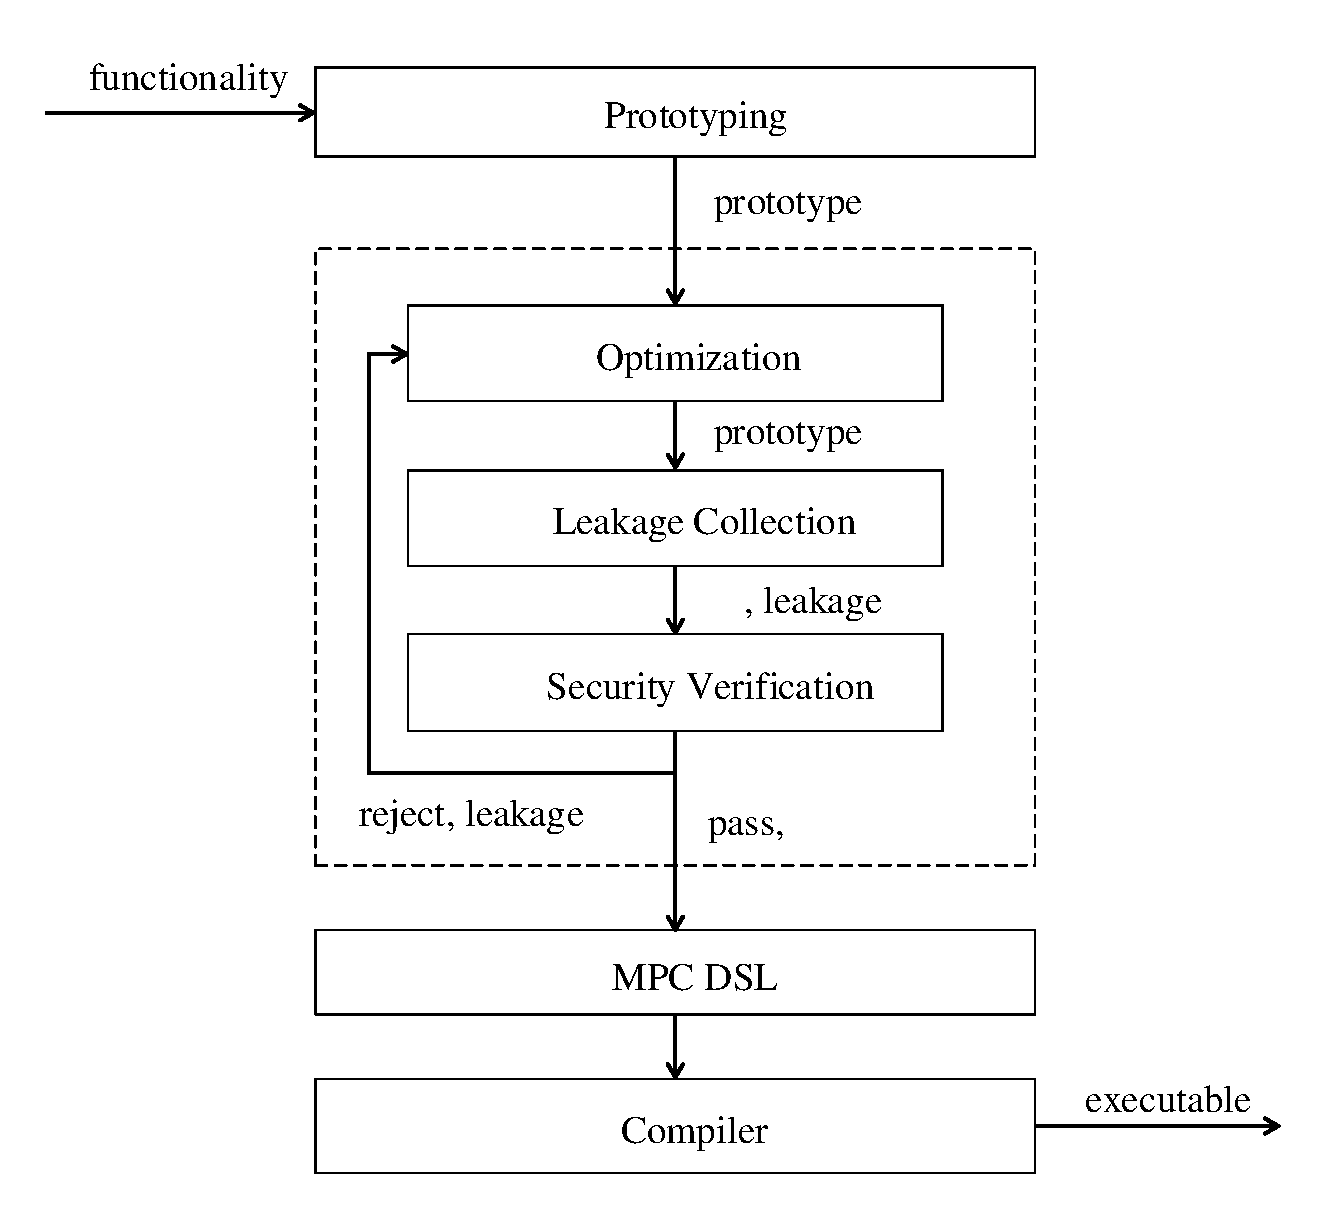
\includegraphics[scale=0.4]{img/workflow.pdf}
    \caption{MPC program development workflow with optimization and verification}
    \label{workflow}
\end{figure}
Our work introduces three parts in the workflow: Optimization, Leakage Collection, and Security Verification.
The optimization part receives a program prototype $p$ which implements the specification including inputs, outputs, functionality $f$ and the \textit{reveal} behavior.
% Programmers reveal some of the intermediate variables in $p$ to reduce the use of oblivious control structures according to our strategy in the optimization part.
The result of the optimization part is $p'$ which is the optimized variant of $p$.
We assume that both $p$ and $p'$ are well-written.
The leakage collection part extracts leakage traces about $p'$ which is modeled in the semantic.
The security verification part verifies the information leakage security of the optimized prototype program $p'$.
The optimized prototype $p'$ will be implemented to practical MPC program if it is secure.
Otherwise, optimized $p'$ has information leakage. Programmers should back to the optimization part and try other optimization.
The complete algorithm of the whole process is as follows \ref{whole}:
\begin{algorithm}[ht]
    \label{whole}
    \caption{Overview}
    \begin{algorithmic}
    \Require Program $p$
    \Ensure $p'$ is leakage secure
    \State log = None
    \While {True}
        \State $p'$ = Optimization($p$, log)
        \State $\Phi$ = Collector($p'$)
        \State secure, log = Verification($p'$, $\Phi$)
        \If {secure}
            \State \Return $p'$
        \EndIf
    \EndWhile
    \end{algorithmic}
\end{algorithm}

\subsection{Optimization}
A straightforward way to improve the performance of MPC program is to reduce the gates of the circuit required by evaluating the MPC program.
According to our observation of MPC, revealing some of the intermediate variables can reduce the use of oblivious control structures so that reduce the size of the circuit.
At the same time, the security is not weakened by the appropriate selection of the intermediate variables to be revealed to ensure that no information leakage is caused.

In the language model in Figure \ref{syntax} and \ref{semantic}, the above strategy is achieved by revealing the oblivious condition variable of obliv if-statement and transferring the obliv if-statement to an if-statement.
The performance of MPC protocols in the real world depends on various factors such as protocol type, CPU performance, network bandwidth, and network latency, so we cannot give a universal optimal strategy.
We allow programmers to transform arbitrary obliv if-statements of a program to if-statements.
The next two parts guarantee the information leakage of the optimized program by verification.

\subsection{Leakage Collection}
We have modeled the information leakage of MPC programs in Section \ref{preli}.
We use a symbolic execution-based approach to extract leakage from MPC programs.
The Algorithm \ref{collect} shows the skeleton of our leakage collector.
The collector extracts leakage trace and leakage lower bound from program $p$.
Algorithm \ref{collect} interprets program $p$ on symbolic memory $\sigma$.
Leakage trace $\phi$ is a sequence of information leakage of an execution path.
$\Phi$ is the set of all leakage traces. $\Phi[\MPCState{y}{\sigma}]$ is the sequence of leakage trace $\phi$ of execution paths whose result is $\MPCState{y}{\sigma}$.
$\Psi$ is the leakage lower bound which is in constraint form in the algorithm.
$\Psi[\MPCState{y}{\sigma}]$ build the constraint for equivalence class $[\thicksim_l]$ where $l=\textit{Eq}(expr_y, \MPCState{y}{\sigma})$.
\begin{algorithm}
    \label{collect}
    \caption{Collector }
    \begin{algorithmic}
    \Require Program $p$, Symbolic memory $\sigma$, Leakage $\phi$, $\psi$
    \Ensure Leakage trace set $\Phi$, Leakage lower bound $\Psi$
    \If {$\MPCAngle{p}$ == $\MPCAngle{\text{skip}}$}
        \State $\Phi$[$\MPCState{y}{\sigma}$].append($\phi$)
        \State $\Psi$[$\MPCState{y}{\sigma}$] =  $\Psi$[$\MPCState{y}{\sigma}$] $\lor$ $\psi$
    \ElsIf{$\MPCAngle{p}$ == $\MPCAngle{\text{skip};p_1}$}
        \State Collector($p_1,\sigma, \phi$)
    \ElsIf {$\MPCAngle{p}$ == $\MPCAngle{lv = e;p_1}$}
        \State Collector($p_1,\sigma[lv\mapsto \MPCState{e}{\sigma}], \phi$)
    \ElsIf {$\MPCAngle{p}$ == $\MPCAngle{lv = \textit{reveal } e;p_1}$}
        \State $\phi$.append($\textit{Eq}(expr_{lv},\MPCState{e}{\sigma})$)
        \State Collector($p_1,\sigma[lv\mapsto \MPCState{e}{\sigma}], \phi$)
    \ElsIf {$\MPCAngle{p}$ == $\MPCAngle{\text{[Obliv] if } e \text{ then } p_1 \text{ else } p_2;p_3}$}
        \State $\psi$.append($\textit{Eq}(expr_{e},\MPCState{e}{\sigma})$)
        \If { SAT$(\MPCState{e}{\sigma})$  }
            \State Collector($p_1;p_3, \sigma, \phi$)
        \EndIf
        \If { SAT$(\MPCState{\text{not }e}{\sigma})$}
            \State Collector($p_2;p_3,\sigma, \phi$)
        \EndIf
    \ElsIf {$\MPCAngle{p}$ == $\MPCAngle{\text{while } e \text{ do } p_1 ; p_2}$}
        \State $\psi$.append($\textit{Eq}(expr_{e},\MPCState{e}{\sigma})$)
        \If {SAT$(\MPCState{e}{\sigma})$}
            \State Collector($p_1;\text{while } e \text{ do } p_1; p_2,\sigma,\phi$)
        \Else {}
            \State Collector($p_2;\sigma,\phi$)
        \EndIf
    \EndIf
    \State \Return $\Phi$, $\Psi$
    \end{algorithmic}
\end{algorithm}
\subsection{Security Verification}
The security should ensure that the leakage of the optimized MPC program $p^\prime$ within the leakage lower bound of the standard MPC program $p$.
The optimized program $p'$ has the same functionality as the standard program $p$.
As we discussed, the leakage lower bound comes from the revealed oblivious result.
Thus, $p$ and $p'$ has the same leakage lower bound.
\begin{theorem}
    MPC programs $p$ and $p'$ have the same leakage lower bound $\Psi$ if they have the same functionality $f$.
\end{theorem}
\begin{proof}
    With the same assumption of private inputs, $p$ has leakge lower bound $\Psi$ and $p'$ has leakage lower bound $\Psi'$.
    Suppose that $\Psi$ and $\Psi'$ are different, then the equivalence class partition of private inputs of $p$ and $p'$ are different.
    The partition is the mapping from private inputs to results, which is exactly the mapping of functionality $f$.
    It contradicts that $p$ and $p'$ have the same functionality $f$.
\end{proof}
\begin{theorem}(Leakage security)
    The leakage of $p'$ is $\Psi^\prime$ and the leakage lower bound of $p'$ is $\Psi$, $p'$ is leakage secure if $\Psi \equiv \Psi'$.
\end{theorem}

\begin{corollary}
    For program $p'$ with private input $x\in X$ and result $y\in Y$, $\Psi \equiv \Psi'$ if and only if $\forall y: \Psi_{y}\equiv\Psi_{y}'$.
\end{corollary}

\begin{corollary}
    For program $p'$ with private input $x\in X$ and result $y\in Y$,
    $\Psi_y \equiv \Psi_y'$ if and only if $\forall \phi\in \Phi[y]: \Psi_{y}\equiv\Psi_{y}\land \phi $.
\end{corollary}

Simplify the condition as:
\begin{equation}
    \begin{split}
    &\Psi_y \equiv \Psi_y' \\
    \Leftrightarrow & \forall{\phi\in \Phi[y]}: \Psi_y \equiv \Psi_y\land \phi  \\
    \Leftrightarrow & \forall{\phi\in \Phi[y]}: \neg (\Psi_y \oplus (\Psi_y\land \phi ))\\
    \Leftrightarrow & \forall{\phi\in \Phi[y]}: \neg (\Psi_y \land (\neg \Psi_y \lor \neg \phi)) \\
    \Leftrightarrow & \forall{\phi\in \Phi[y]}: \neg \Psi_y \lor \phi \\
\end{split}
\end{equation}
As we verify the partition of case $y$, the $\Psi_y$ holds. So:
\begin{equation}
    \label{simend}
    \begin{split}
    &\Psi_y \models  \forall{\phi\in \Phi[y]}: \neg \Psi_y \lor \phi \\
    \Leftrightarrow & \Psi_y \models \forall{\phi\in \Phi[y]}: \phi \\
    \Leftrightarrow & \Psi_y \models \bigwedge_{\phi\in \Phi[y]} \phi \\
\end{split}
\end{equation}
For each constraint of $\Psi$, we verify the condition in Eq. \ref{simend} to ensure that the partition corresponding to this constraint holds in $p'$.
The algorithm of verification process is in Algorithm \ref{algo-verify}.
\begin{algorithm}
    \label{algo-verify}
    \caption{Verification }
    \begin{algorithmic}
    \Require Leakage lower bound $\Psi$, Leakage trace $\Phi$
    \Ensure Pass or Reject
    \State log = None
    \For {each $y \in Y$}
        \State b = Solver($\Psi_y \models \bigwedge_{\phi\in \Phi[y]} \phi$)
        \If {$\neg$b}
            \State \Return Reject
        \EndIf
    \EndFor
    \State \Return Pass
    \end{algorithmic}
\end{algorithm}

% \begin{proof}(Soundness)
%     For program $p'$ with private input $x\in X$ and result $y\in Y$,
%     When $p'$ pass verification process, we have $y\in Y$, $\Psi_y \equiv \Psi_y'$ for any $y$.
%     Thus, $\Psi \equiv\Psi'$, $p'$ is leakage secure.
% \end{proof}

\begin{theorem}(Semi-honest security)
    For program $p$ with private input $x\in X$ and result $y\in Y$, suppose $p$ has leakage $\Psi$ and is secure against a semi-honest adversary.
    For program $p'$ with private input $x\in X$ and result $y\in Y$, if $p'$ has information leakage $\Psi$, $p'$ is secure against the semi-honest adversary.
\end{theorem}
\begin{proof}
\textit{sketch.}
In the ideal world, the simulator knows the partition corresponding to the private inputs.
Suppose $TTP$ in the ideal world gets result $y$. The simulator knows that the constraint is $\Psi_y$.
During the simulation of $View_{\text{sim},adv}^{p'}$, each time a intermediate variable $v$ are revealed, the simulator check the satisfiable of $\Psi_y\land Eq(expr_v, true)$.
If so, the simulator send a message such that the decrypt of $v$ is true. Otherwise, the simulator send a massage such that the decrypt of $v$ is false.


Consider the ideal world vs. real world paradigm of program $p$, the adversary's view in the real world is $View_{\text{real},adv}^{p}$ , in the ideal world is $View_{\text{sim},adv}^{p}$. $p$ is secure against the semi-honest adversary, so the distributions of $View_{\text{real},adv}^{p}$  and $View_{\text{sim},adv}^{p}$ are indistinguishable to the adversary. For program $p'$, suppose the distributions of $View_{\text{real},adv}^{p'}$  and $View_{\text{sim},adv}^{p'}$  are distinguishable. The adversary has to obey the protocol to execute $p'$ without any active behavior such as interrupt the protocol, send spurious messages and so on. In this situation, The difference between $View_{adv}^{p'}$ and $View_{adv}^{p}$ is the revealed control flow information $\psi_e$ for each execution. The view of $\psi_e$ for the distribution of $View_{adv}^{p'}$ is the combination form $\bigwedge_{pt}\psi_{pt}$. Thus, $View_{adv}^{p'}$ becomes distinguishable due to the knowledge $\bigwedge_{pt}\psi_{pt}$. However, we have proved that $ \neg \Psi_y \lor \bigwedge_{pt\in Path(y)} \psi_{pt}\Leftrightarrow\Psi_y\rightarrow \bigwedge_{pt\in Path(y)}\psi_{pt}$ , and $\Psi$ is also learnt from $View_{adv}^{p}$. Thus, $View_{adv}^{p}$ is distinguishable. However, it is contradict to the assumption that $p'$ is secure against the semi-honest adversary. Therefore, $View_{\text{real},adv}^{p'}$ and $View_{\text{sim},adv}^{p'}$ are indistinguishable, and $p'$ is secure against the semi-honest adversary.
\end{proof}

\section{Implementation and Evaluation}\label{sec:implementation}
%\subsection{Implementation}
\begin{figure}[t]
	\centering
	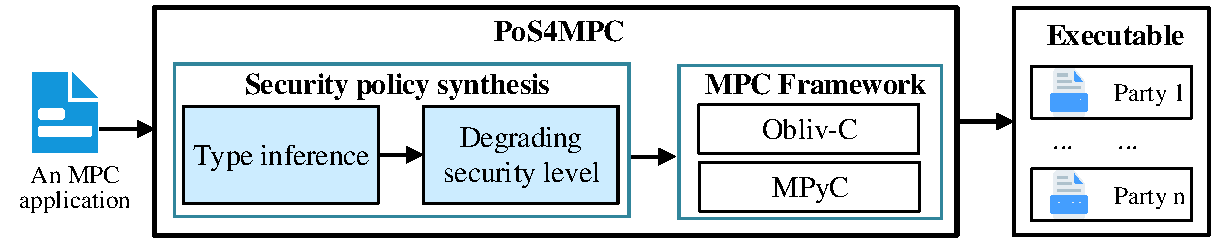
\includegraphics[scale=0.56]{img/workflow-v1}
	\vspace{-2mm}
	\caption{The workflow of our tool \TNAME}
	\label{fig-impl}
	\vspace{-3mm}
\end{figure}
We have implemented our approach in a tool, named \TNAME. The workflow of \TNAME is shown in Fig.~\ref{fig-impl},
The input is an MPC program in C, which is parsed %the C program to construct its
to an intermediate representation (IR)
inside the LLVM Compiler~\cite{llvm} where call graph and control flow graphs are constructed %via LLVM passes
at the LLVM IR level.
We then perform the type inference which computes
the a perfect security policy for the given program.
To be accurate, we perform a field-sensitive pointer
analysis~\cite{BalatsourasS16} and our type inference is also field-sensitive.
As the next step, we leverage the KLEE symbolic execution engine~\cite{CadarDE08}
to explore all the feasible symbolic executions, as well as the symbolic
values of the return variable and secret branching variables of each symbolic execution.
Based on them, we iteratively check if a secret branching variable % specified by the security policy
can be declassified.  %until no more can be declassified, during which
If it is the case, its security level %of the found secret branching variable
is degraded and the result is fed back to the type inference to refine security levels before checking the next secret branching variable.
%in the security policy if it does not compromise security.
After that, we transform the program into the input of Obliv-C~\cite{ZahurE15} by which the program can be compiled into
executable implementations, one for each party. Obliv-C is an extension of C for implementing 2-party MPC applications using Yao's garbled circuit protocol~\cite{yao82}.
For experimental purposes, \TNAME also features the high-level MPC framework MPyC~\cite{MPyC20},
which is a Python package for implementing $n$-party MPC applications ($n\geq 1$) using Shamir's secret sharing protocol~\cite{Shamir79}.
The C program is transformed into Python by a translator~\cite{C2Python}.

We also implement an optimization in our tool to alleviate the path explosion problem. Instead of directly checking the validity of $\Psi_x(t,t')$
for each secret branching variable $x$ and pair of symbolic executions $t$ and $t'$,
we first check if the premise $\phi\wedge \Primed(\phi')\wedge e=\Primed(e')$
of $\Psi_x(t,t')$ is satisfiable. We can conclude that $\Psi_x(t,t')$ is valid for any secret branching variable $x$ if the premise $\phi\wedge \Primed(\phi')\wedge e=\Primed(e')$ is unsatisfiable.
Furthermore, this yields a sound compositional reasoning approach which allows to split
a program into a sequence of function calls. When each pair of the symbolic executions
for each function cannot result in the same return value, we can conclude that
$\Psi_x(t,t')$ is valid for any secret branching variable $x$ and any pair of symbolic executions $t$ and $t'$
of the entire program.


%
% automatic verification tool \TNAME based on the symbolic engine KLEE.
%Figure \ref{fig-impl} shows the workflow of \TNAME.
%Fortunately, the symbolic and concrete variables give a fine mapping to secret and public variables.
%We simplify the implementation of \TNAME by regarding symbolic variables as secret variables, and concrete values as public data.
%The input of \TNAME is the program $p$.
%The collector of \TNAME fully explores all reachable paths of the given program to extract the conditions.
%\TNAME constructs the leakage lower bound and the leakage of the given program and then generates queries of the constraint solver to accomplish verification.
%\TNAME will output a hint indicating the insecure case if the program fails the verification.

\subsection{Evaluation Setup}\label{sec:experiments}
%In this section, we evaluate the efficiency and effectiveness of our approach and the performance improvement of
%MPC applications with our security policies.


%
%\smallskip
%\noindent
%{\bf Benchmarks.}
For an evaluation of our approach, we conduct experiments on five typical 2-party MPC applications~\cite{benchmarks}, i.e.,
quicksort ({\tt QS})~\cite{mpcqsort}, linear search ({\tt LinS})~\cite{absent}, binary search  ({\tt BinS})~\cite{absent},
  almost search ({\tt AlmS})~\cite{Knuth73},
and  private set intersection  ({\tt PSI})~\cite{Andreea21}.
%Taking a private array $\vec{a}_i$ of integers from each party $\Party{i}$ as input,
%which forms one array $\vec{a}$ where the first half is $\vec{a}_1$
%and the second half is $\vec{a}_2$,
{\tt QS} outputs the list of indices of a given integer array $\vec{a}$ in its ordered version, where
the first half of $\vec{a}$ is given by one party and the second half of $\vec{a}$ is given by the another party.
{\tt LinS} (resp. {\tt BinS} and {\tt AlmS}) outputs the index
of an integer $b$ in an array $\vec{a}$ if it exists, $-1$ otherwise, where
the integer array $\vec{a}$ is the input from one party and the integer $b$ is the input from
the another party.
{\tt LinS} always scans the array from the start to the end even though it has found the integer $b$.
{\tt BinS} is a standard iterative approach on a sorted array, where the array index is protected via oblivious read access machine~\cite{GoldreichO96}.
{\tt AlmS} is a variant of {\tt BinS}, where the input array is almost sorted, namely,
each element is at either the correct position or the closest neighbour
of the correct position.
{\tt PSI} outputs the intersection of two integer sets, each of which
is an input from one party.

All the experiments were conducted on a desktop with 64-bit Linux Mint 20.1, Intel Core i5-6300HQ CPU, 2.30 GHz and 8 GB RAM. When evaluating MPC applications, the client of each party
is executed with a single thread.
%The speedup is calculated by the formula $std \ time/opt \ time$.
%The measurement result is the average of 10 times repetitions.


\subsection{Performance of Security Policy Synthesis}
{\bf Security policy}.
The results of our approach is shown in Table~\ref{table:policyresults},
where column (LOC) shows the number of lines of code,
column (\#Branch var) shows the number of branching variables
while column (\#Other var) shows the number of other variables,
columns (After TS) and (After Check) respectively
show the number of secret branching variables after
applying the type system and checking if the secret branching variables can be declassified,
columns (Before refinement) and (After refinement) respectively show
the number of other secret variables before and after refining the type inference by feeding
back the results of the symbolic reasoning.
(Note that the input variables are excluded in counting.)

We can observe that only few variables (2 for \texttt{QS}, 1 for \texttt{LinS}, 2 for \texttt{BinS}, 2 for \texttt{AlmS} and 2 for \texttt{PSI})
can be found to be public by solely using the type system.
With our symbolic reasoning approach, more secret branching variables can be declassified
without compromising the security (3 for \texttt{QS}, 1 for \texttt{LinS}, 1 for \texttt{BinS}, 2 for \texttt{AlmS} and 1 for \texttt{PSI}).
After refining the type inference using results of the symbolic reasoning approach,
more secret variables can be declassified (2 for \texttt{QS}, 1 for \texttt{LinS} and 2 for \texttt{PSI}).
Overall, our approach annotates 2, 1, 7, 12 and 1 internal variables as secret out of
10, 4, 10, 16 and 6 variables for \texttt{QS}, \texttt{LinS}, \texttt{BinS}, \texttt{AlmS} and \texttt{PSI}, respectively.
%
%Our security policy synthesis securely declassifies 3 (resp. 1, 1, 1, 1) secret conditions at
%{\tt QS}'s Line 17, 21, 31 (resp. {\tt LinS}'s Line 9, {\tt BinS}'s Line 30, {\tt AlmS}'s Line 29, {\tt PSI}'s Line 9), while {\tt QS} (resp. {\tt LinS}, {\tt BinS}, {\tt AlmS}, {\tt PSI})
%contains 3 (resp. 1, 2, 6, 1) secret conditions. In detail,
%{\tt QS} declassifies the comparisons of the pivot and array elements,
%{\tt LinS} (resp. {\tt PSI}) declassifies the equality of the search value and array elements,
%{\tt BinS} (resp. {\tt AlmS}) declassifies the equality of the search value and array's boundary value in each iteration.
%Furthermore, with declassifing above secret conditions, the partition result of {\tt QS} become public so that no secret indexes for array access.
%The {\tt LinS} (resp. {\tt BinS}, {\tt AlmS}) can early return its result once it find the search value.
%The {\tt PSI} can jump to next loop round once it find a intersection value. Overall, {\tt QS} (resp. {\tt LinS}, {\tt BinS}, {\tt AlmS}, {\tt PSI}) reduces more computations, not only the secret conditional branches.
%

\smallskip
\noindent
{\bf Execution time}. The execution time of our approach is shown in Table~\ref{table:policytime},
where columns (SE) and (Check) respectively show the execution time (in second unless indicated by h for hour) of collecting symbolic executions
and checking if secret branching variables can be declassified, by varying
the size of the input array for each program from 10 to 100 with step 10.
We did not report the execution time of our type system, as
it is less than 0.1 second for each benchmark.

\begin{table}[t]
    \centering
    \scalebox{0.8}{
    \begin{tabular}{|c|c|c|c|c|c|c|c|}
    \hline
    \multirow{2}{*}{\bf Name} & \multirow{2}{*}{\bf LOC} & \multirow{2}{*}{\bf \#Branch var} & \multirow{2}{*}{\bf \#Other var}& \multicolumn{2}{c|}{\bf \#Secret branch var} & \multicolumn{2}{c|}{\bf \#Other secret var} \\     \cline{5-8}                                                                                                                                                                                                                                                                                                                                   &            &                                       &   & After TS & After Check  & Before refinement & After refinement\\ \hline
   {\bf QS}    & 56  & 4 & 6  &  3 & 0    & 4  & 2    \\ \hline
   {\bf LinS}  & 25  & 1 & 3  &  1 & 0    & 2  & 1   \\ \hline
   {\bf BinS}  & 46  & 2 & 8  &  2 & 1    & 6  & 6     \\ \hline
   {\bf AlmS}  & 73  & 6 & 10 &  6 & 4    & 8  & 8      \\ \hline
   {\bf PSI}   & 34  & 1 & 5  &  1 & 0    & 3  & 1 \\ \hline
    \end{tabular}
    }
    \caption{Number of (secret) branching variables}
    \label{table:policyresults}\vspace{-6mm}
\end{table}

\begin{table}[t]
\centering
    \scalebox{0.65}{
    \begin{tabular}{|c|cccccccccccccccccccc|}
    \hline
    \multirow{3}{*}{\bf Name}  & \multicolumn{20}{c|}{\bf  Length}                                                                                                                                                                                                                                                                                                                                                 \\ \cline{2-21}
                         & \multicolumn{2}{c|}{10}             & \multicolumn{2}{c|}{20}            & \multicolumn{2}{c|}{30}            & \multicolumn{2}{c|}{40}             & \multicolumn{2}{c|}{50}             & \multicolumn{2}{c|}{60}             & \multicolumn{2}{c|}{70}             & \multicolumn{2}{c|}{80}             & \multicolumn{2}{c|}{90}             & \multicolumn{2}{c|}{100} \\ \cline{2-21}
                            & {SE}    & \multicolumn{1}{c|}{Check} & {SE}   & \multicolumn{1}{c|}{Check} & {SE}   & \multicolumn{1}{c|}{Check} & {SE}    & \multicolumn{1}{c|}{Check} & {SE}    & \multicolumn{1}{c|}{Check} & {SE}    & \multicolumn{1}{c|}{Check} & {SE}    & \multicolumn{1}{c|}{Check} & {SE}    & \multicolumn{1}{c|}{Check} & {SE}    & \multicolumn{1}{c|}{Check} & {SE}         & {Check}      \\ \hline
   {\bf QS}                  & 11.6 & \multicolumn{1}{c|}{0.8}   & 0.4h & \multicolumn{1}{c|}{304.2} & 2.0h & \multicolumn{1}{c|}{959.8} & 5.0h  & \multicolumn{1}{c|}{0.6h}   & 9.5h  & \multicolumn{1}{c|}{0.9h}   & 15.5h & \multicolumn{1}{c|}{1.3h}   & 22.6h & \multicolumn{1}{c|}{1.6h}   & 31.0h & \multicolumn{1}{c|}{2.0h}   & 40.7h & \multicolumn{1}{c|}{2.3h}   & 51.6h      & 2.7h        \\ \hline
   {\bf LinS}                  & 0.4  & \multicolumn{1}{c|}{1.0}   & 0.6 & \multicolumn{1}{c|}{1.0}   & 1.0 & \multicolumn{1}{c|}{1.0}   & 1.4  & \multicolumn{1}{c|}{1.0}   & 2.0  & \multicolumn{1}{c|}{1.1}   & 2.6  & \multicolumn{1}{c|}{1.1}   & 3.4  & \multicolumn{1}{c|}{1.2}   & 4.2  & \multicolumn{1}{c|}{1.2}   & 5.2  & \multicolumn{1}{c|}{1.3}   & 6.2       & 1.4        \\ \hline
   {\bf BinS}                 & 0.8  & \multicolumn{1}{c|}{1.1}   & 2.1 & \multicolumn{1}{c|}{4.3}   & 3.8 & \multicolumn{1}{c|}{10.2}  & 6.4  & \multicolumn{1}{c|}{20.0}  & 9.5  & \multicolumn{1}{c|}{34.8}  & 13.8 & \multicolumn{1}{c|}{54.6}  & 19.5 & \multicolumn{1}{c|}{80.1}  & 25.6 & \multicolumn{1}{c|}{103.4} & 34.1 & \multicolumn{1}{c|}{151.4} & 42.7      & 204.7      \\ \hline
   {\bf AlmS}                 & 1.3  & \multicolumn{1}{c|}{0.8}   & 4.3 & \multicolumn{1}{c|}{3.5}   & 7.7 & \multicolumn{1}{c|}{10.0}  & 14.1 & \multicolumn{1}{c|}{18.6}  & 20.6 & \multicolumn{1}{c|}{32.3}  & 28.9 & \multicolumn{1}{c|}{51.0}  & 40.7 & \multicolumn{1}{c|}{77.4}  & 55.1 & \multicolumn{1}{c|}{110.3} & 74.9 & \multicolumn{1}{c|}{148.2} & 94.4      & 200.0      \\ \hline
   {\bf PSI}                  & 1.7  & \multicolumn{1}{c|}{0.5}   & 4.3 & \multicolumn{1}{c|}{1.0}   & 8.0 & \multicolumn{1}{c|}{1.5}   & 13.2 & \multicolumn{1}{c|}{2.1}   & 20.0 & \multicolumn{1}{c|}{2.8}   & 28.6 & \multicolumn{1}{c|}{3.5}   & 39.3 & \multicolumn{1}{c|}{4.3}   & 50.9 & \multicolumn{1}{c|}{5.3}   & 63.0 & \multicolumn{1}{c|}{6.4}   & 79.6      & 7.8        \\ \hline
    \end{tabular}
    }
    \caption{Execution time of our security policy synthesis approach}
    \label{table:policytime}
  \vspace{-7mm}
\end{table}

%\begin{table}[t]
%    \scalebox{0.62}{
%    \begin{tabular}{|c|c|c|ccccccccccccccccccc|}
%    \hline
%    \multirow{3}{*}{\bf Name}  & \multirow{3}{*}{\bf TS} & \multicolumn{20}{c|}{\bf  Length}                                                                                                                                                                                                                                                                                                                                                 \\ \cline{3-22}
%                          &         & \multicolumn{2}{c|}{10}             & \multicolumn{2}{c|}{20}            & \multicolumn{2}{c|}{30}            & \multicolumn{2}{c|}{40}             & \multicolumn{2}{c|}{50}             & \multicolumn{2}{c|}{60}             & \multicolumn{2}{c|}{70}             & \multicolumn{2}{c|}{80}             & \multicolumn{2}{c|}{90}             & \multicolumn{2}{c|}{100} \\ \cline{3-22}
%                          &          & {SE}    & \multicolumn{1}{c|}{Check} & {SE}   & \multicolumn{1}{c|}{Check} & {SE}   & \multicolumn{1}{c|}{Check} & {SE}    & \multicolumn{1}{c|}{Check} & {SE}    & \multicolumn{1}{c|}{Check} & {SE}    & \multicolumn{1}{c|}{Check} & {SE}    & \multicolumn{1}{c|}{Check} & {SE}    & \multicolumn{1}{c|}{Check} & {SE}    & \multicolumn{1}{c|}{Check} & {SE}         & {Check}      \\ \hline
%   {\bf QS}               & 0.049               & 11.6 & \multicolumn{1}{c|}{0.8}   & 0.4h & \multicolumn{1}{c|}{304.2} & 2.0h & \multicolumn{1}{c|}{959.8} & 5.0h  & \multicolumn{1}{c|}{0.6h}   & 9.5h  & \multicolumn{1}{c|}{0.9h}   & 15.5h & \multicolumn{1}{c|}{1.3h}   & 22.6h & \multicolumn{1}{c|}{1.6h}   & 31.0h & \multicolumn{1}{c|}{2.0h}   & 40.7h & \multicolumn{1}{c|}{2.3h}   & 51.6h      & 2.7h        \\ \hline
%   {\bf LinS}              & 0.044               & 0.4  & \multicolumn{1}{c|}{1.0}   & 0.6 & \multicolumn{1}{c|}{1.0}   & 1.0 & \multicolumn{1}{c|}{1.0}   & 1.4  & \multicolumn{1}{c|}{1.0}   & 2.0  & \multicolumn{1}{c|}{1.1}   & 2.6  & \multicolumn{1}{c|}{1.1}   & 3.4  & \multicolumn{1}{c|}{1.2}   & 4.2  & \multicolumn{1}{c|}{1.2}   & 5.2  & \multicolumn{1}{c|}{1.3}   & 6.2       & 1.4        \\ \hline
%   {\bf BinS}             & 0.048               & 0.8  & \multicolumn{1}{c|}{1.1}   & 2.1 & \multicolumn{1}{c|}{4.3}   & 3.8 & \multicolumn{1}{c|}{10.2}  & 6.4  & \multicolumn{1}{c|}{20.0}  & 9.5  & \multicolumn{1}{c|}{34.8}  & 13.8 & \multicolumn{1}{c|}{54.6}  & 19.5 & \multicolumn{1}{c|}{80.1}  & 25.6 & \multicolumn{1}{c|}{103.4} & 34.1 & \multicolumn{1}{c|}{151.4} & 42.7      & 204.7      \\ \hline
%   {\bf AlmS}            & 0.062               & 1.3  & \multicolumn{1}{c|}{0.8}   & 4.3 & \multicolumn{1}{c|}{3.5}   & 7.7 & \multicolumn{1}{c|}{10.0}  & 14.1 & \multicolumn{1}{c|}{18.6}  & 20.6 & \multicolumn{1}{c|}{32.3}  & 28.9 & \multicolumn{1}{c|}{51.0}  & 40.7 & \multicolumn{1}{c|}{77.4}  & 55.1 & \multicolumn{1}{c|}{110.3} & 74.9 & \multicolumn{1}{c|}{148.2} & 94.4      & 200.0      \\ \hline
%   {\bf PSI}              & 0.048               & 1.7  & \multicolumn{1}{c|}{0.5}   & 4.3 & \multicolumn{1}{c|}{1.0}   & 8.0 & \multicolumn{1}{c|}{1.5}   & 13.2 & \multicolumn{1}{c|}{2.1}   & 20.0 & \multicolumn{1}{c|}{2.8}   & 28.6 & \multicolumn{1}{c|}{3.5}   & 39.3 & \multicolumn{1}{c|}{4.3}   & 50.9 & \multicolumn{1}{c|}{5.3}   & 63.0 & \multicolumn{1}{c|}{6.4}   & 79.6      & 7.8        \\ \hline
%    \end{tabular}
%    }
%    \caption{Execution time of our security policy synthesis approach}
%    \label{Table:results}
%    \centering
%\end{table}

%
%\BEGIN{TABLE}[T]
%    \SCALEBOX{0.6}{
%    \BEGIN{TABULAR}{|C|C|C|CCCCCCCCCCCCCCCCCCCC|}
%    \HLINE
%    \MULTIROW{3}{*}{\BF nAME} & \MULTIROW{3}{*}{\BF  loc} & \MULTIROW{3}{*}{\BF ts} & \MULTICOLUMN{20}{C|}{\BF  lENGTH}                                                                                                                                                                                                                                                                                                                                                 \\ \CLINE{4-23}
%                          &                        &                     & \MULTICOLUMN{2}{C|}{10}             & \MULTICOLUMN{2}{C|}{20}            & \MULTICOLUMN{2}{C|}{30}            & \MULTICOLUMN{2}{C|}{40}             & \MULTICOLUMN{2}{C|}{50}             & \MULTICOLUMN{2}{C|}{60}             & \MULTICOLUMN{2}{C|}{70}             & \MULTICOLUMN{2}{C|}{80}             & \MULTICOLUMN{2}{C|}{90}             & \MULTICOLUMN{2}{C|}{100} \\ \CLINE{4-23}
%                          &                        &                     & {se}    & \MULTICOLUMN{1}{C|}{cHECK} & {se}   & \MULTICOLUMN{1}{C|}{cHECK} & {se}   & \MULTICOLUMN{1}{C|}{cHECK} & {se}    & \MULTICOLUMN{1}{C|}{cHECK} & {se}    & \MULTICOLUMN{1}{C|}{cHECK} & {se}    & \MULTICOLUMN{1}{C|}{cHECK} & {se}    & \MULTICOLUMN{1}{C|}{cHECK} & {se}    & \MULTICOLUMN{1}{C|}{cHECK} & {se}    & \MULTICOLUMN{1}{C|}{cHECK} & {se}         & {cHECK}      \\ \HLINE
%   {\BF qs}                    & 64                     & 0.049               & 11.6 & \MULTICOLUMN{1}{C|}{0.8}   & 0.4H & \MULTICOLUMN{1}{C|}{304.2} & 2.0H & \MULTICOLUMN{1}{C|}{959.8} & 5.0H  & \MULTICOLUMN{1}{C|}{0.6H}   & 9.5H  & \MULTICOLUMN{1}{C|}{0.9H}   & 15.5H & \MULTICOLUMN{1}{C|}{1.3H}   & 22.6H & \MULTICOLUMN{1}{C|}{1.6H}   & 31.0H & \MULTICOLUMN{1}{C|}{2.0H}   & 40.7H & \MULTICOLUMN{1}{C|}{2.3H}   & 51.6H      & 2.7H        \\ \HLINE
%   {\BF lINs}               & 27                     & 0.044               & 0.4  & \MULTICOLUMN{1}{C|}{1.0}   & 0.6 & \MULTICOLUMN{1}{C|}{1.0}   & 1.0 & \MULTICOLUMN{1}{C|}{1.0}   & 1.4  & \MULTICOLUMN{1}{C|}{1.0}   & 2.0  & \MULTICOLUMN{1}{C|}{1.1}   & 2.6  & \MULTICOLUMN{1}{C|}{1.1}   & 3.4  & \MULTICOLUMN{1}{C|}{1.2}   & 4.2  & \MULTICOLUMN{1}{C|}{1.2}   & 5.2  & \MULTICOLUMN{1}{C|}{1.3}   & 6.2       & 1.4        \\ \HLINE
%   {\BF bINs}                 & 53                     & 0.048               & 0.8  & \MULTICOLUMN{1}{C|}{1.1}   & 2.1 & \MULTICOLUMN{1}{C|}{4.3}   & 3.8 & \MULTICOLUMN{1}{C|}{10.2}  & 6.4  & \MULTICOLUMN{1}{C|}{20.0}  & 9.5  & \MULTICOLUMN{1}{C|}{34.8}  & 13.8 & \MULTICOLUMN{1}{C|}{54.6}  & 19.5 & \MULTICOLUMN{1}{C|}{80.1}  & 25.6 & \MULTICOLUMN{1}{C|}{103.4} & 34.1 & \MULTICOLUMN{1}{C|}{151.4} & 42.7      & 204.7      \\ \HLINE
%   {\BF aLMs}                  & 80                     & 0.062               & 1.3  & \MULTICOLUMN{1}{C|}{0.8}   & 4.3 & \MULTICOLUMN{1}{C|}{3.5}   & 7.7 & \MULTICOLUMN{1}{C|}{10.0}  & 14.1 & \MULTICOLUMN{1}{C|}{18.6}  & 20.6 & \MULTICOLUMN{1}{C|}{32.3}  & 28.9 & \MULTICOLUMN{1}{C|}{51.0}  & 40.7 & \MULTICOLUMN{1}{C|}{77.4}  & 55.1 & \MULTICOLUMN{1}{C|}{110.3} & 74.9 & \MULTICOLUMN{1}{C|}{148.2} & 94.4      & 200.0      \\ \HLINE
%   {\BF psi}                   & 36                     & 0.048               & 1.7  & \MULTICOLUMN{1}{C|}{0.5}   & 4.3 & \MULTICOLUMN{1}{C|}{1.0}   & 8.0 & \MULTICOLUMN{1}{C|}{1.5}   & 13.2 & \MULTICOLUMN{1}{C|}{2.1}   & 20.0 & \MULTICOLUMN{1}{C|}{2.8}   & 28.6 & \MULTICOLUMN{1}{C|}{3.5}   & 39.3 & \MULTICOLUMN{1}{C|}{4.3}   & 50.9 & \MULTICOLUMN{1}{C|}{5.3}   & 63.0 & \MULTICOLUMN{1}{C|}{6.4}   & 79.6      & 7.8        \\ \HLINE
%    \END{TABULAR}
%    }
%    \CAPTION{eXECUTION TIME OF OUR SECURITY POLICY SYNTHESIS APPROACH}
%    \LABEL{tABLE:SPS}
%    \CENTERING
%\END{TABLE}

We can observe that our symbolic reasoning approach is able to check
all the secret branching variables in few minutes (up to 294.4s)
except for {\tt QS}.
After an in-depth analysis, we found that the number of symbolic executions is exponential in the length
of the input array for {\tt QS} and {\tt PSI}
while it is linear in the length of the input array for the other benchmarks.
Our compositional reasoning approach works very well
on {\tt PSI}, otherwise it would take similar execution time
as on {\tt QS}. Indeed, a loop of {\tt PSI} is implemented as a sequence of function calls each of which has a fixed number of symbolic executions.
Furthermore, each pair of symbolic executions in the called function cannot result in the same return value.
Therefore, the number of symbolic executions and the execution time of our symbolic reasoning approach is reduced significantly.
However, our compositional reasoning approach does not work
on {\tt QS}. Although the number of symbolic executions grows exponentially on {\tt QS},
the execution time of checking if secret branching variables can be declassified
is still reduced by our optimization, which avoids the checking of the constraint $\Psi_x(t,t')$
if its premise $\phi\wedge \Primed(\phi')\wedge e=\Primed(e')$ is unsatisfiable.


%
%
%As the result, the security policy synthesis of QS (resp. LinS, BinS, AlmS, PSI) takes 19.0h (resp. 3.8s, 82.2s, 99.3s, 34.2s) on average.
%QS takes significantly more time due to the path explosion problem, the number of execution paths of QS is factorial to its input array size.
%The number of execution paths of LinS (resp. BinS, AlmS) is linear to its input array size.
%But BinS (resp. AlmS) contains more branches and assumptions about the input than LinS.
%Thus, the symbolic execution of BinS (resp. AlmS) takes more time to determine the reachability of a new path when exploring program paths.
%To avoid PSI's exponential number of execution paths,
%we unroll PSI's bounded loop and split PSI into a sequence of function calls as PSI calls linear scan per loop.
%We verified each function call cannot result in the same return value.
%Therefore, the SE and Verify of PSI are much faster than QS. We have also optimized the QS policy synthesis.
%To fully explore QS's execution path, there are O(n2) calls of the partition function.
%However, most partition calls have the same input array length except the values of arrays are different.
%We verify every possible partition call with different lengths in {\tt QS}, and verified any partition call cannot result in the same state of {\tt QS}'s output.
%Above optimization eliminates duplicate symbolic execution and only needs $O(n)$ times of partition calls.
%Although we mitigate the path explosion problem of {\tt QS}, we cannot fully eliminate it due to the partition process's path explosion problem.
%
%Our security policy synthesis securely declassifies 3 (resp. 1, 1, 1, 1) secret conditions at
%{\tt QS}'s Line 17, 21, 31 (resp. {\tt LinS}'s Line 9, {\tt BinS}'s Line 30, {\tt AlmS}'s Line 29, {\tt PSI}'s Line 9), while {\tt QS} (resp. {\tt LinS}, {\tt BinS}, {\tt AlmS}, {\tt PSI})
%contains 3 (resp. 1, 2, 6, 1) secret conditions. In detail,
%{\tt QS} declassifies the comparisons of the pivot and array elements,
%{\tt LinS} (resp. {\tt PSI}) declassifies the equality of the search value and array elements,
%{\tt BinS} (resp. {\tt AlmS}) declassifies the equality of the search value and array's boundary value in each iteration.
%Furthermore, with declassifing above secret conditions, the partition result of {\tt QS} become public so that no secret indexes for array access.
%The {\tt LinS} (resp. {\tt BinS}, {\tt AlmS}) can early return its result once it find the search value.
%The {\tt PSI} can jump to next loop round once it find a intersection value. Overall, {\tt QS} (resp. {\tt LinS}, {\tt BinS}, {\tt AlmS}, {\tt PSI}) reduces more computations, not only the secret conditional branches.
%


\subsection{Performance Improvement of MPC Applications}
To evaluate the performance improvement of the MPC applications,
we compare the execution time (in second), the size of the circuits (in $10^6\times$gates), and
the volume of communication traffic (in MB) of each benchmark with the security policies v1 and v2,
where v1 is obtained by solely applying our type system
and v2 is obtained from v1 by degrading security levels and refinement
without compromising the security.
The measurement results are given as the average of 10 times repetitions in order to minimize
noises.

\begin{figure}[t]
    \centering
    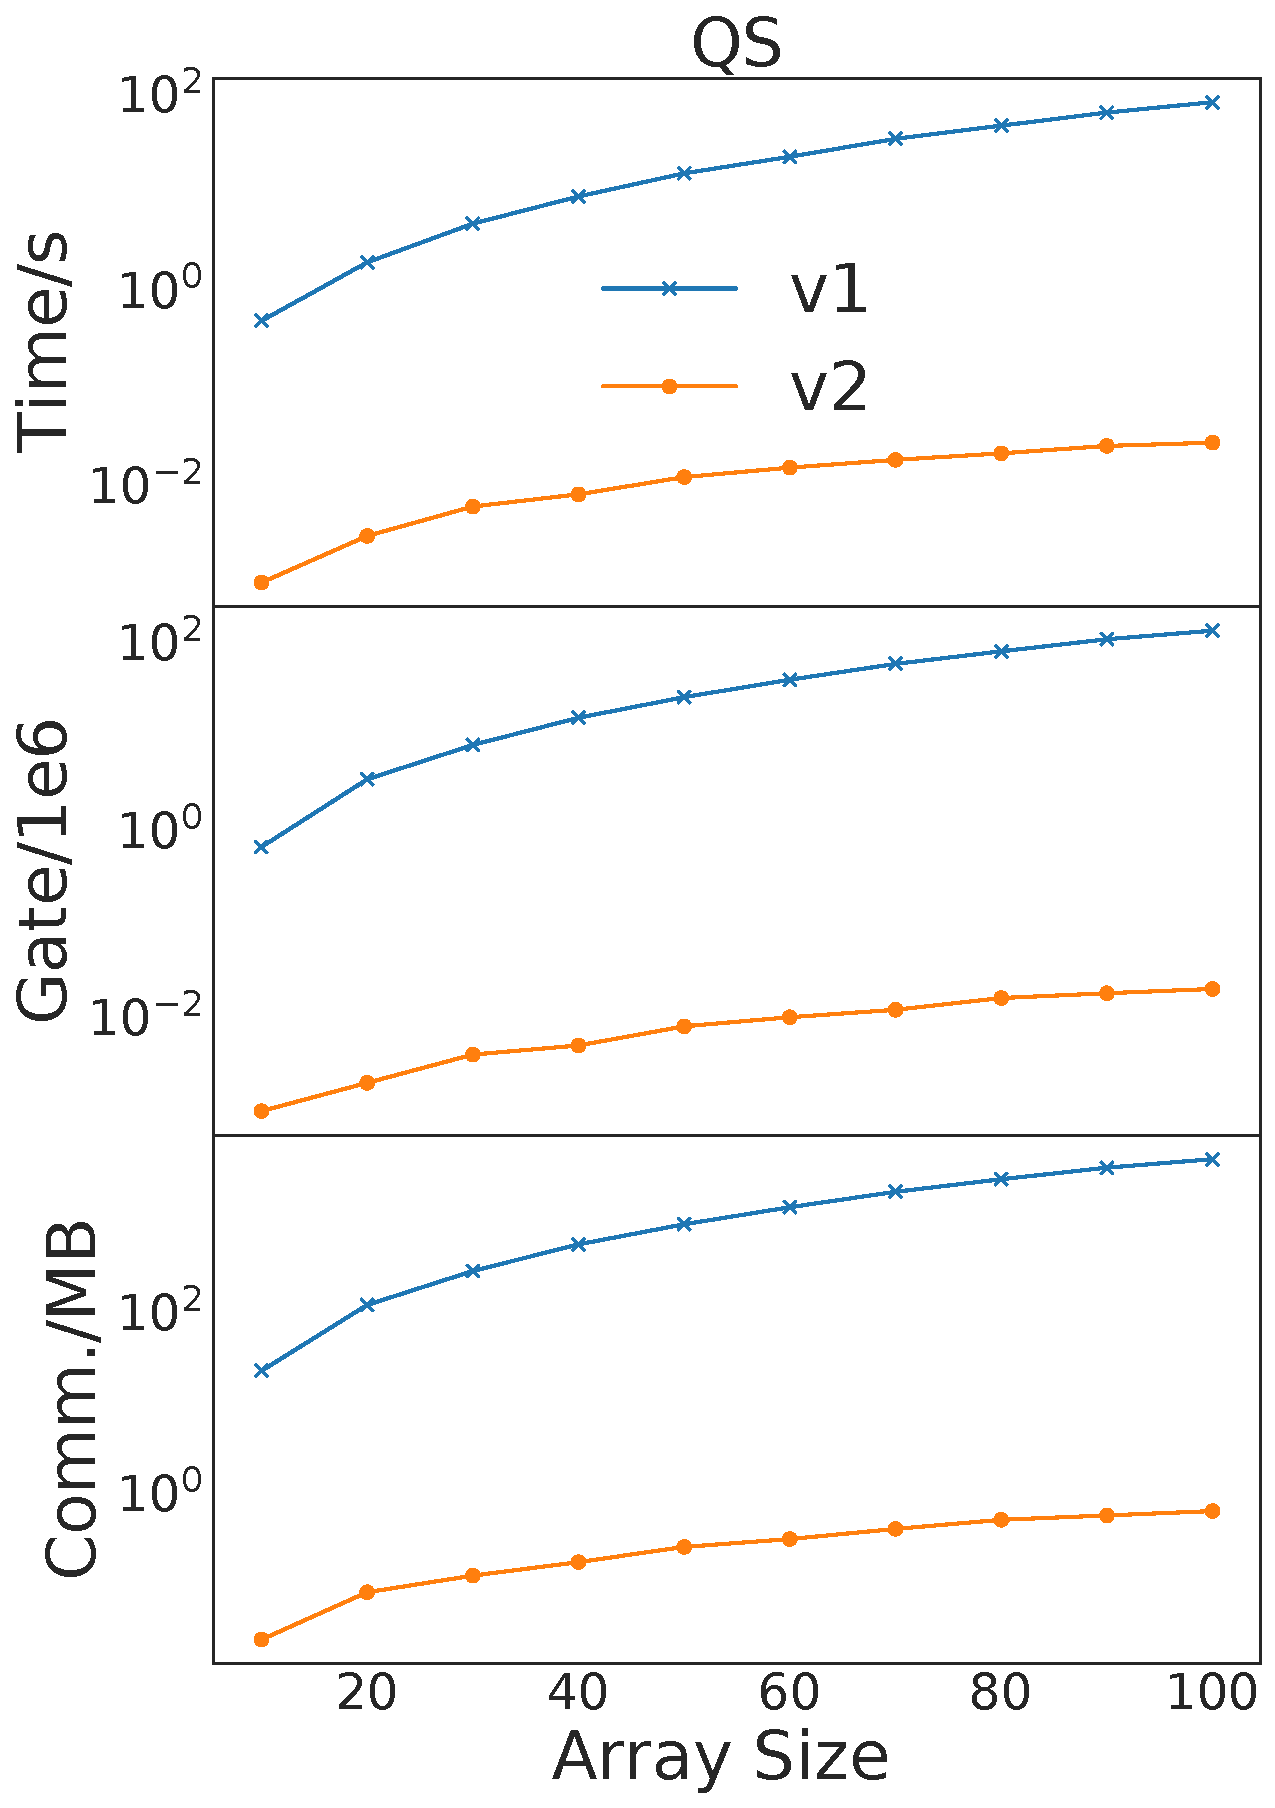
\includegraphics[width=0.24\textwidth]{img/gc100Left}
    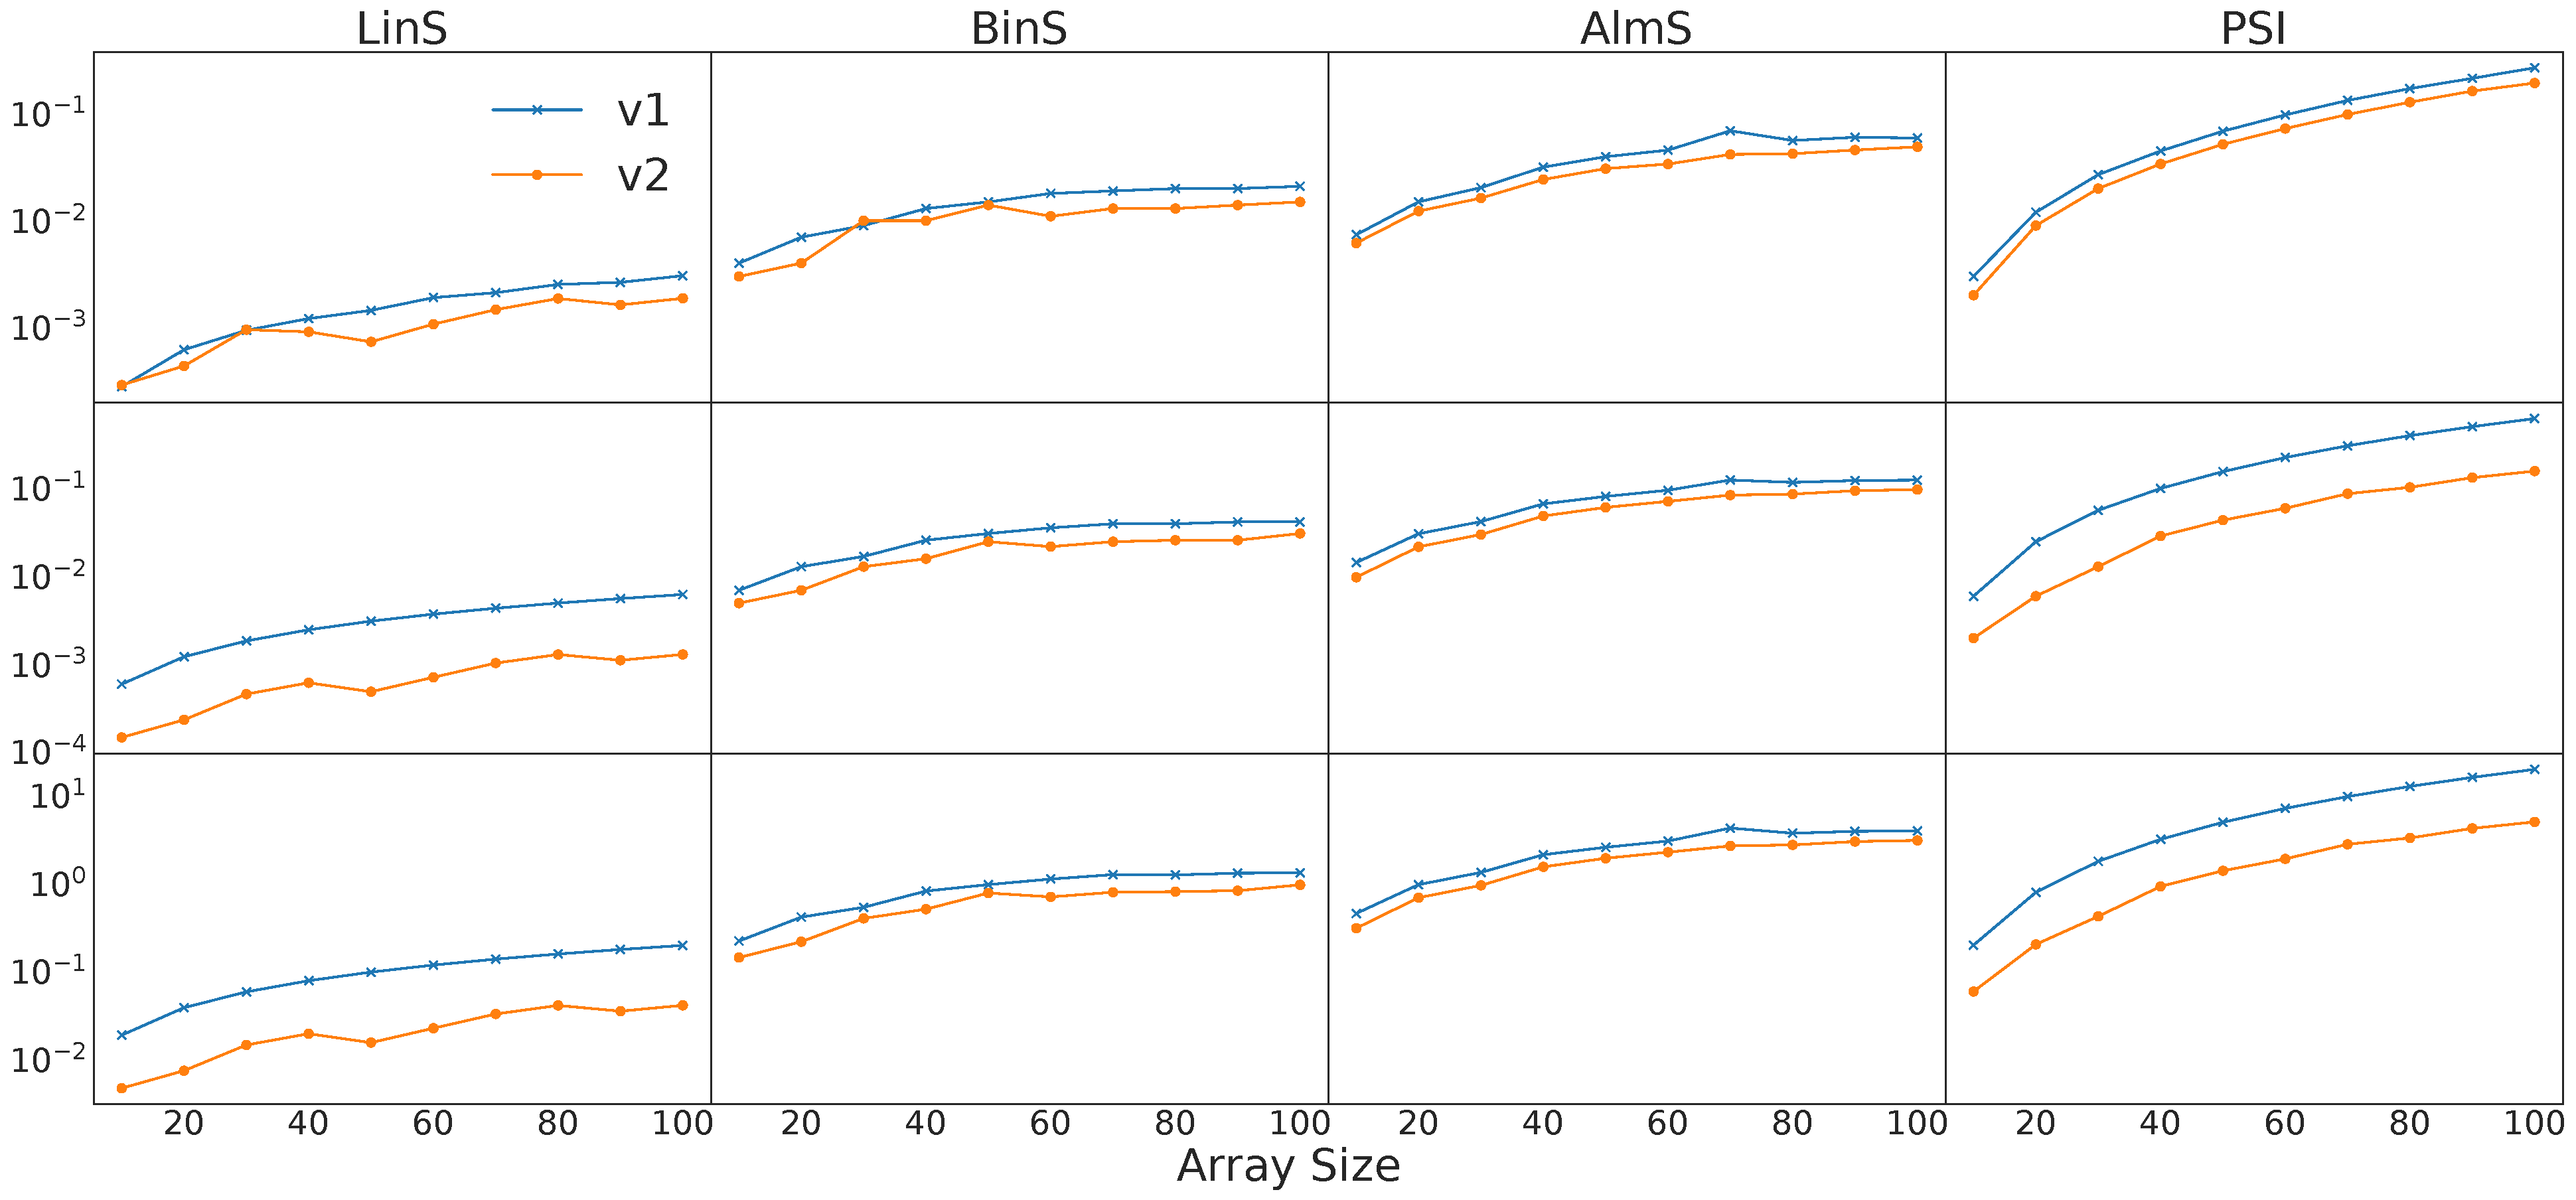
\includegraphics[width=0.74\textwidth]{img/gc100Right}
    \vspace{-1mm}
    \caption{Execution time (Time) in second, the number of gates (Gate) in 1e6 gates, Communication (Comm.) in MB using Obliv-C}
    \label{fig:gc}  \vspace{-2mm}
\end{figure}

\smallskip
\noindent
{\bf By Obliv-C.} The results in Obliv-C are depicted in Fig.~\ref{fig:gc}, where
the size of the random input array for each benchmark varies from 10 to 100 with step 10.
Overall, we can observe that the performance improvement is significant, in particular,
on {\tt QS}.
%
In detail, compared over the security policy v1 on {\tt QS} (resp. {\tt LinS}, {\tt BinS}, {\tt AlmS}, and {\tt PSI}),
on average, the security policy v2 reduces (1) the execution time by $1.56\times 10^5\%$ (resp. $45\%$, $38\%$, $31\%$ and $36\%$),
(2) the size of circuits by $3.61\times 10^5\%$ (resp. $368\%$, $52\%$, $38\%$ and $275\%$),
and (3) the volume of communication traffic by $4.17\times 10^5\%$ (resp. $367\%$, $53\%$, $39\%$ and $274\%$).
This demonstrates the performance improvement of the MPC applications
in  Obliv-C that uses Yao's garbled circuit protocol.

\begin{figure}[t]
    \centering
    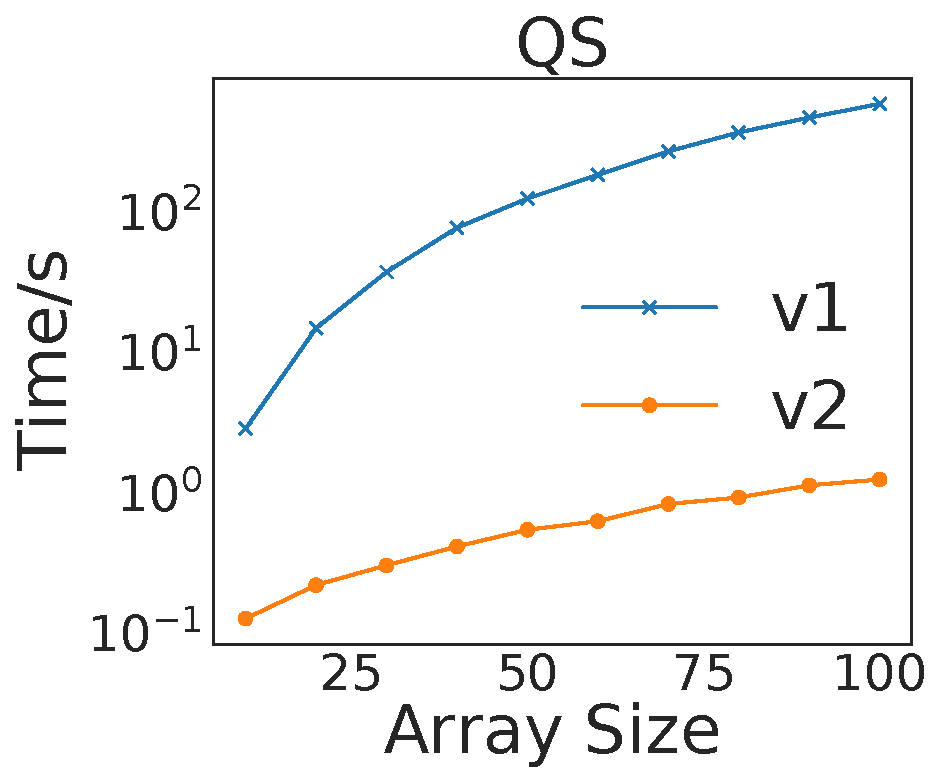
\includegraphics[width=0.24\textwidth]{img/ss100Left}
    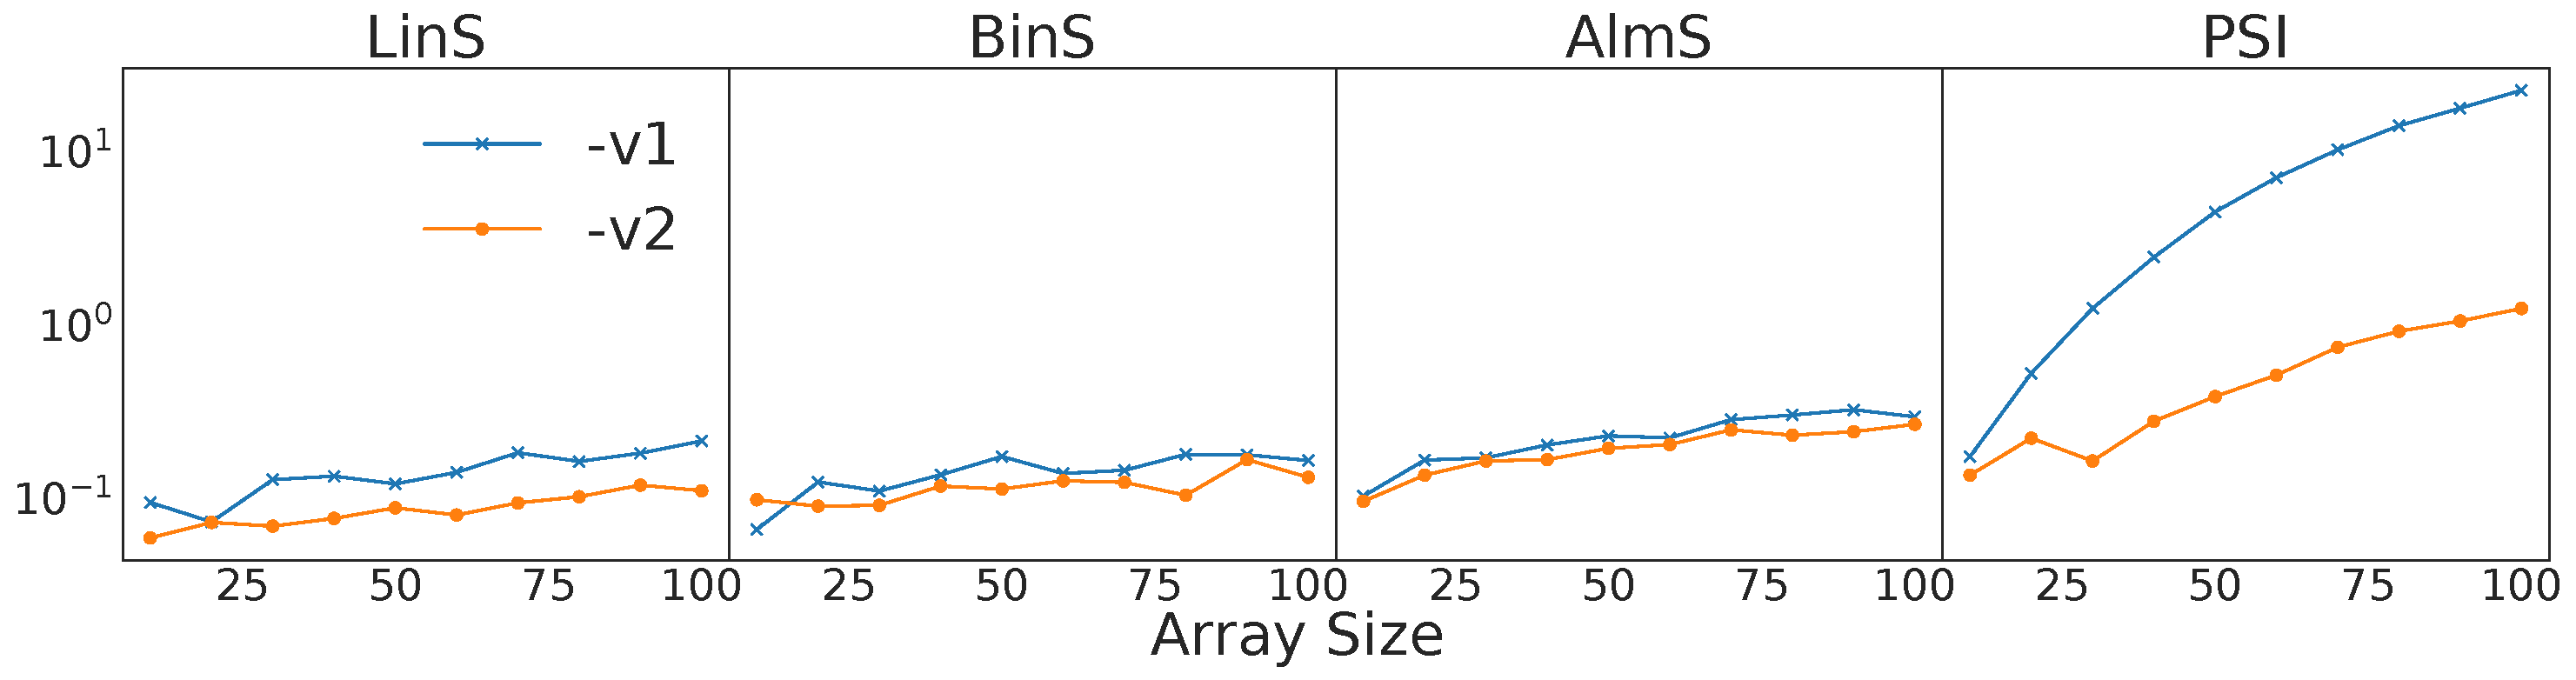
\includegraphics[width=0.7515\textwidth]{img/ss100Right}
   \vspace{-5mm} \caption{Execution time (Time) in second using MPyC}
    \label{fig:ss}  \vspace{-4mm}
\end{figure}

\smallskip
\noindent
{\bf By MPyC.} The results in MPyC are depicted in Fig.~\ref{fig:ss}.
Since  MPyC does not provide the size of circuits and the volume of communication traffic, we only report
execution time in Fig.~\ref{fig:ss}.
The results show that degrading security levels also improves execution time
in MPyC that uses Shamir's secret sharing protocol.
Compared over the security policy v1 on benchmark {\tt QS} (resp. {\tt LinS}, {\tt BinS}, {\tt AlmS}, and {\tt PSI}), on average the security policy v2 reduces the execution time by $2.5\times 10^4\%$ (resp. $64\%$, $23\%$, $17\%$ and $996\%$).


\begin{comment}

\smallskip
\noindent
{\bf Comparing with Batcher Bitonic sorting.}


We experiment our optimization approach and verification tool on 6 pairs of study cases.
The experiment result shows that our verification tool verifies a program within seconds.
Our optimization approach reduces 25\% to 91\% circuit size and communications and achieves 1.25$\times$ to 3.84$\times$ performance speedup in Yao's garbled circuit protocol, 1.25$\times$ to 24.14$\times$ speedup in Shamir's secret sharing protocol.


\subsubsection{Environment setting}
All of our experiments are implemented on a Linux desktop with 2.30 GHz CPU and 8 GB memory.
We run clients of parties on the same machine with a single thread for each client.
The speedup is calculated by the formula $std \ time/opt \ time$.
The measurement result is the average of 10 times repetitions.

We fully implement all study case programs in two real-world MPC frameworks: Obliv-C and MPyC.
Obliv-C implements Yao's garbled circuit protocol.
MPyC implements Shamir's secret sharing protocol.
We survey many MPC frameworks for our experiments.
It is disappointing that we cannot implement our all study cases on frameworks \cite{spdz,aby2,sharemind}.
They compile the whole circuit before protocol execution.
So we cannot use runtime information to avoid useless computations in them.


\subsubsection{Study cases}
To our knowledge, no program set contains many MPC application implementations.
So we collect six programs as study cases from the literature and open source project \cite{ZahurE15,absent,mpcqsort}.
We optimize the programs by our strategy and verify their leakage security.
All opt programs are verified that they are leakage secure.
We call the original version of a study case program as std and the optimized version of a study case program as opt.

The first study case is MPC sorting.
The sorting program receives two private integer arrays and outputs the ordered indexes of each array item.
We compare our optimized sorting program with the state-of-the-art MPC sorting program.
The std program is an implementation of Batcher sort that is the most popular sorting algorithm in MPC applications.
The opt program is an implementation of quicksort.
An oblivious quicksort has seriously poor performance due to the oblivious of control flow.
We optimize oblivious quicksort to a significant improvement.
Our optimization is similar to \cite{mpcqsort} but without the random shuffle because we prove its security.

The MPC searching study case searches an integer in an array and outputs its index if found.
The group of searching programs has three different algorithms.
Linear search is a commonly used algorithm in MPC programs.
The std program scans the array from the start to the end even though it has found the element.
Our opt program reveals the comparison result of the std.
Once the opt finds the element, it terminates immediately.
Binary search is a standard iterative implementation.
The std program accesses array items by oblivious index,
so it uses oblivious RAM to avoid leaking oblivious index.
Our opt program reveals the result of the equality test and terminates once it finds the element.
Almost Search is a variant of Binary Search.
The inputs of the almost search program are almost in order.
An item of the almost ordered array may be at the correct position, or the positions left or right next to the correct position.
The implementation of std and optimization of opt is similar to binary search.

The quadratic PSI computes the intersection of two privacy sets.
% Optimized OT-based PSI protocols \cite{pssz} perform much better than general MPC protocols.
We adopt a naive implementation of PSI to illustrate the effect of our method in the general MPC program.
The opt program reveals the result of the items' equality test.
Once the opt program finds two identical elements, it ignores the remaining comparisons and jumps to the next round to search for the next element.

Line segment intersection program is an application of MPC in computational graphics.
It receives two line segments and outputs the intersection point coordinate if they intersect.
The computation between line segments is float point which is much more expensive than integers in MPC.
Our opt program terminates if two line segments do not intersect while the std program always computes a point by the intersection point formula.
\subsubsection{Verification Result}
\begin{table}[ht]
    \centering
    \caption{Verification Detail}
    \setlength{\tabcolsep}{1mm}
    \begin{tabular}{c|c|c|c|c}
    \hline
    Program           & Input Size        & Partitions & Time/s & Verified \\ \hline
    Quick Sort\cite{mpcqsort}        & 6 int             & 720        & 12.099 & \checkmark      \\ \hline
    Linear Search\cite{absent}     & 16 int            & 17         & 0.432  & \checkmark      \\ \hline
    Binary Search\cite{absent}     & 16 int            & 17         & 1.146  & \checkmark       \\ \hline
    Almost Search     & 16 int            & 17         & 5.183  & \checkmark       \\ \hline
    Line Intersection & 4 float + 4 float & 2          & 1.409  & \checkmark       \\ \hline
    Quadratic PSI     & 4 int + 4 int     & 209        & 7.27   & \checkmark     \\ \hline
    \end{tabular}
    \label{verify}
\end{table}

\begin{table}[ht]
    \centering
    \caption{Program Referemce}
    \setlength{\tabcolsep}{1mm}
    \begin{tabular}{c|c}
    \hline
    Program           & Reference         \\ \hline
    Batcher Sort      & Paper: Sorting networks and their applications\\ \hline
    Linear Search     & Absentminded Crypto Kit:Linear scan of ORAM                \\ \hline
    Binary Search     & Absentminded Crypto Kit: src/osearch.oc                 \\ \hline
    Almost Search     & A variant of Binary search                 \\ \hline
    Quadratic PSI     & A $O(n^2)$ implementation of PSI problem         \\ \hline
    \end{tabular}
\end{table}

Table \ref{verify} shows the verification results.
In practice, the size of the privacy array is public in MPC.
To make the symbolic execution terminates, we limit the size of program inputs.
It is sufficient to say that the verified program is secure on larger inputs size.
In Table \ref{verify}, our verification tool verifies all programs within seconds.
Our verification tool is efficient enough.

\subsubsection{Performance evaluation}

\begin{figure}[h]
    \centering
    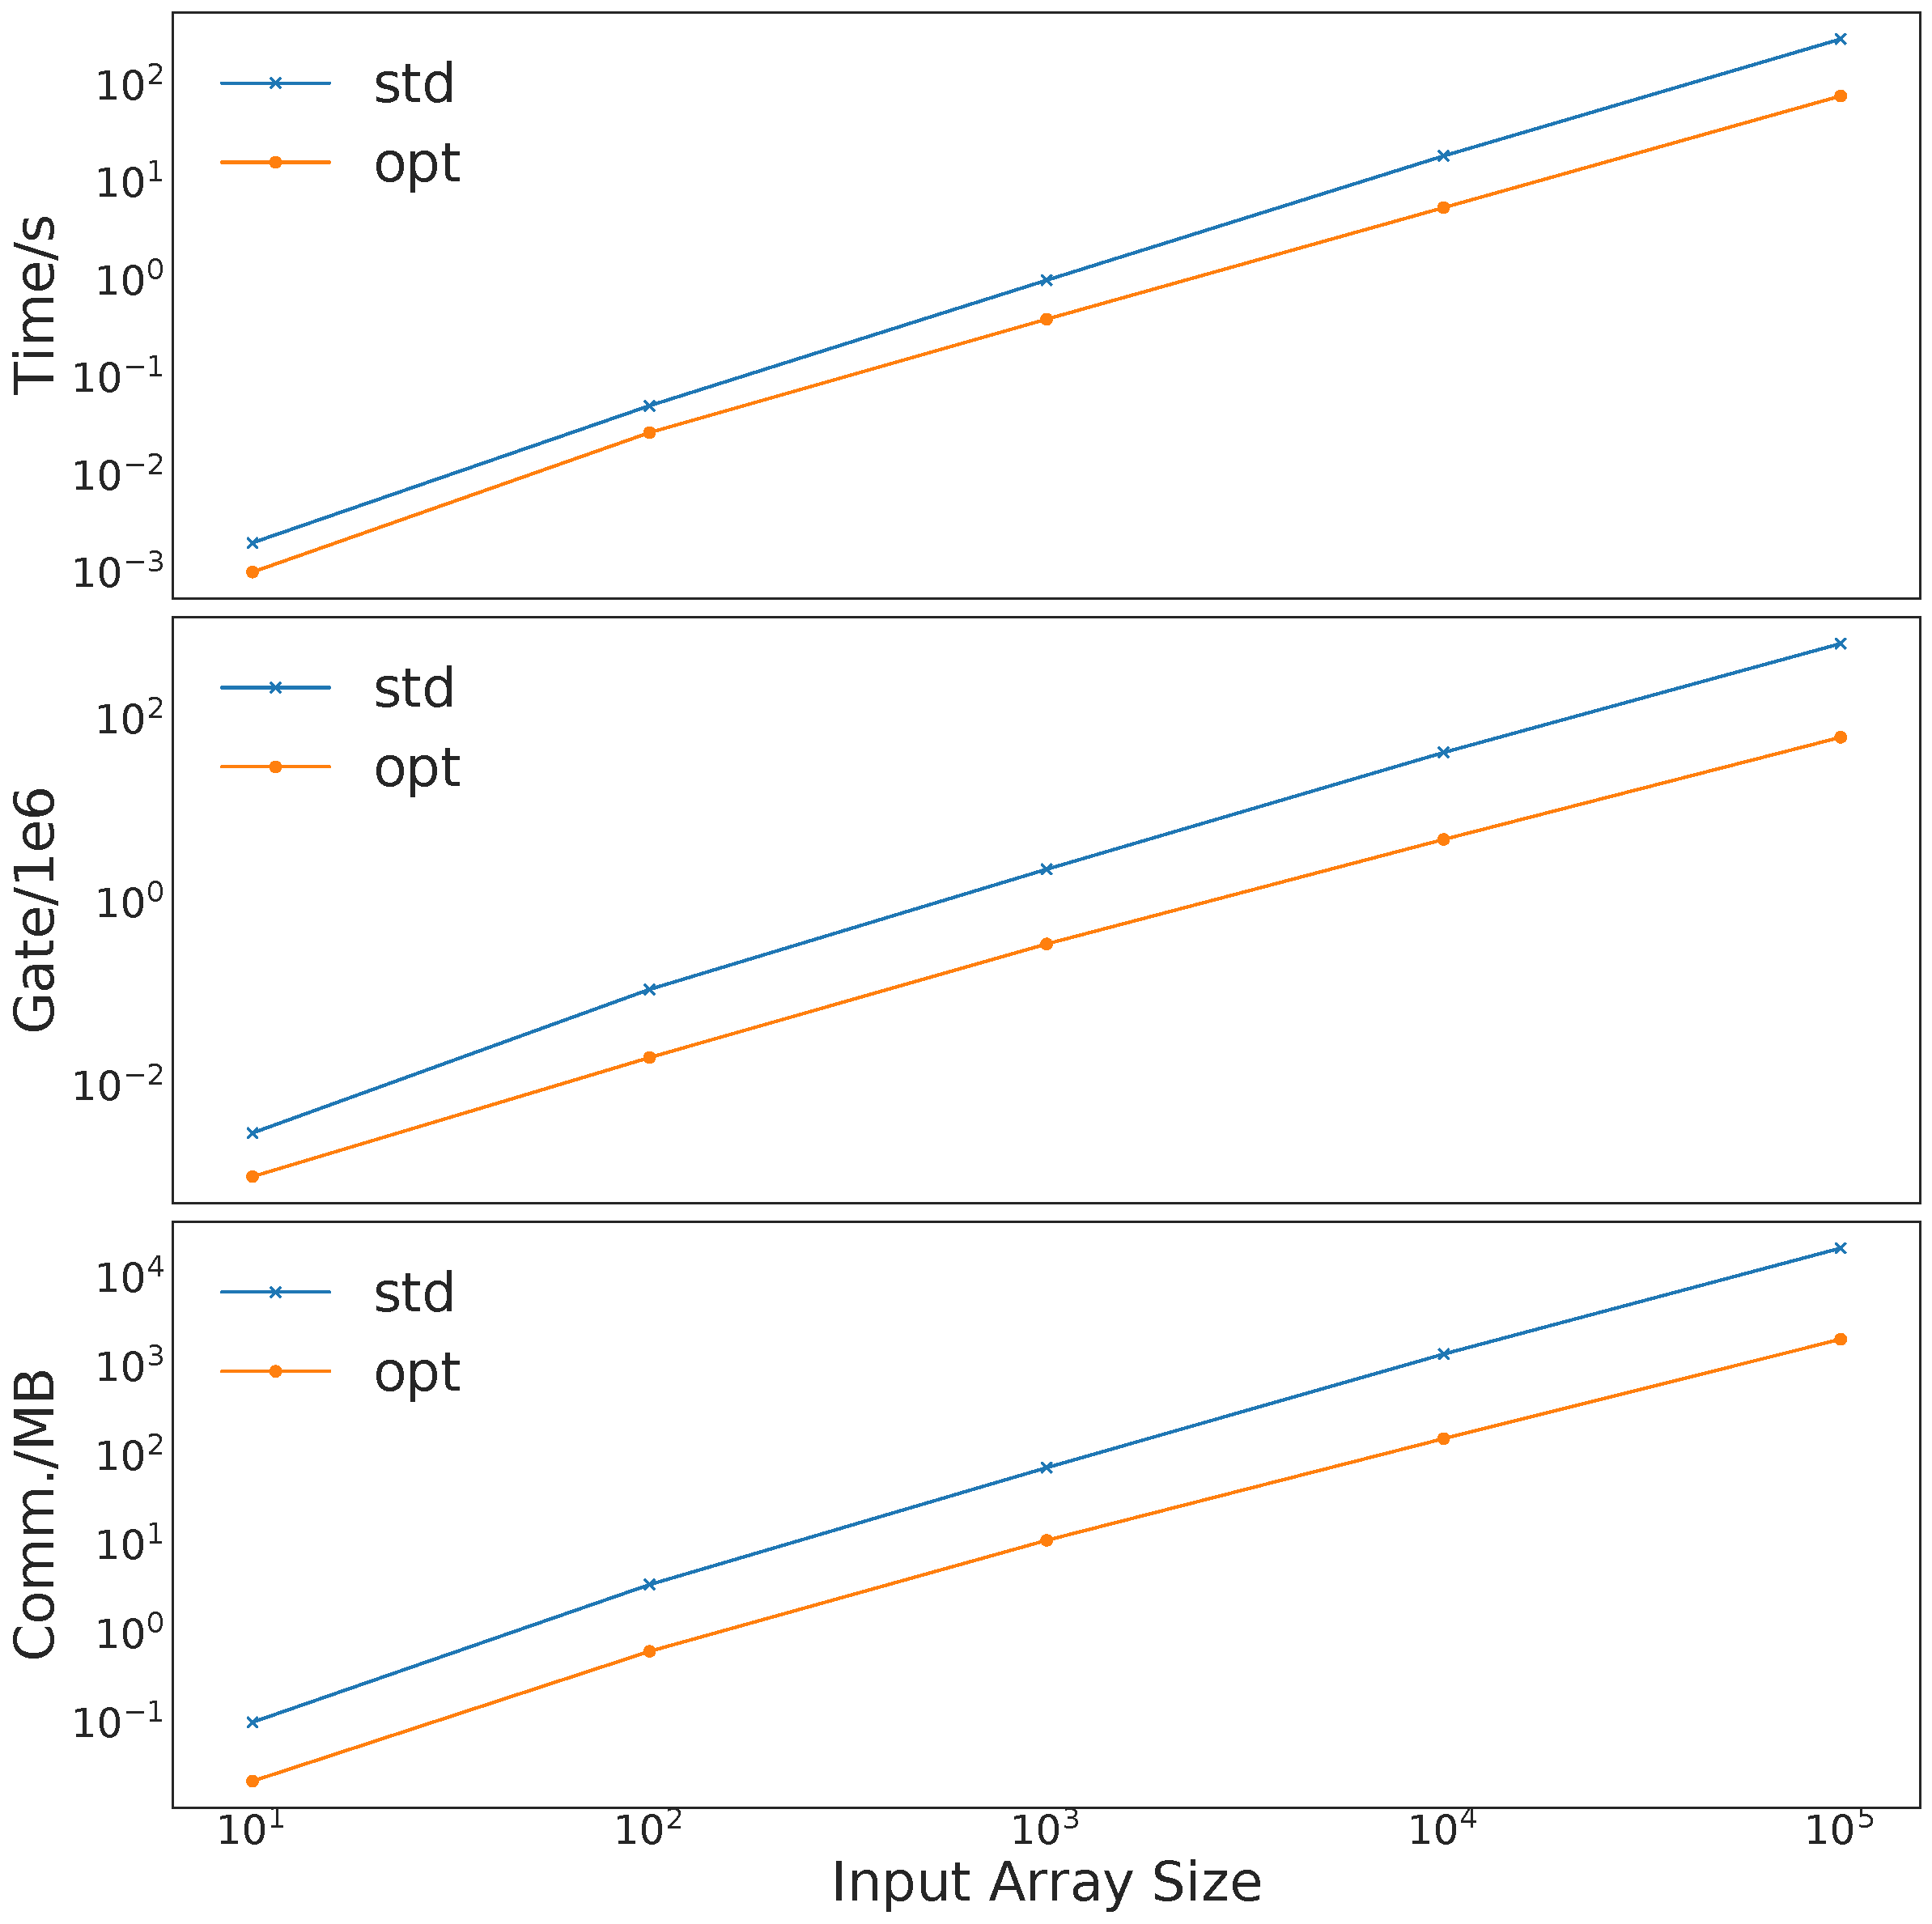
\includegraphics[scale=0.2]{img/gc-sorting.pdf}
    \caption{Communication (Comm.), the number of gates (Gate), protocol execution time (Time) of sorting in Yao's garbled circuit protocol with input array size range from $10^1$ to $10^5$.}
    \label{gcsorting}
\end{figure}
Fig. \ref{gcsorting} shows the performance comparison between sorting std and opt programs in Yao's garbled circuit protocol.

Our opt program reduces 91\% circuit size and communications and achieves 3.84$\times$ speedup.
\begin{figure}[h]
    \centering
    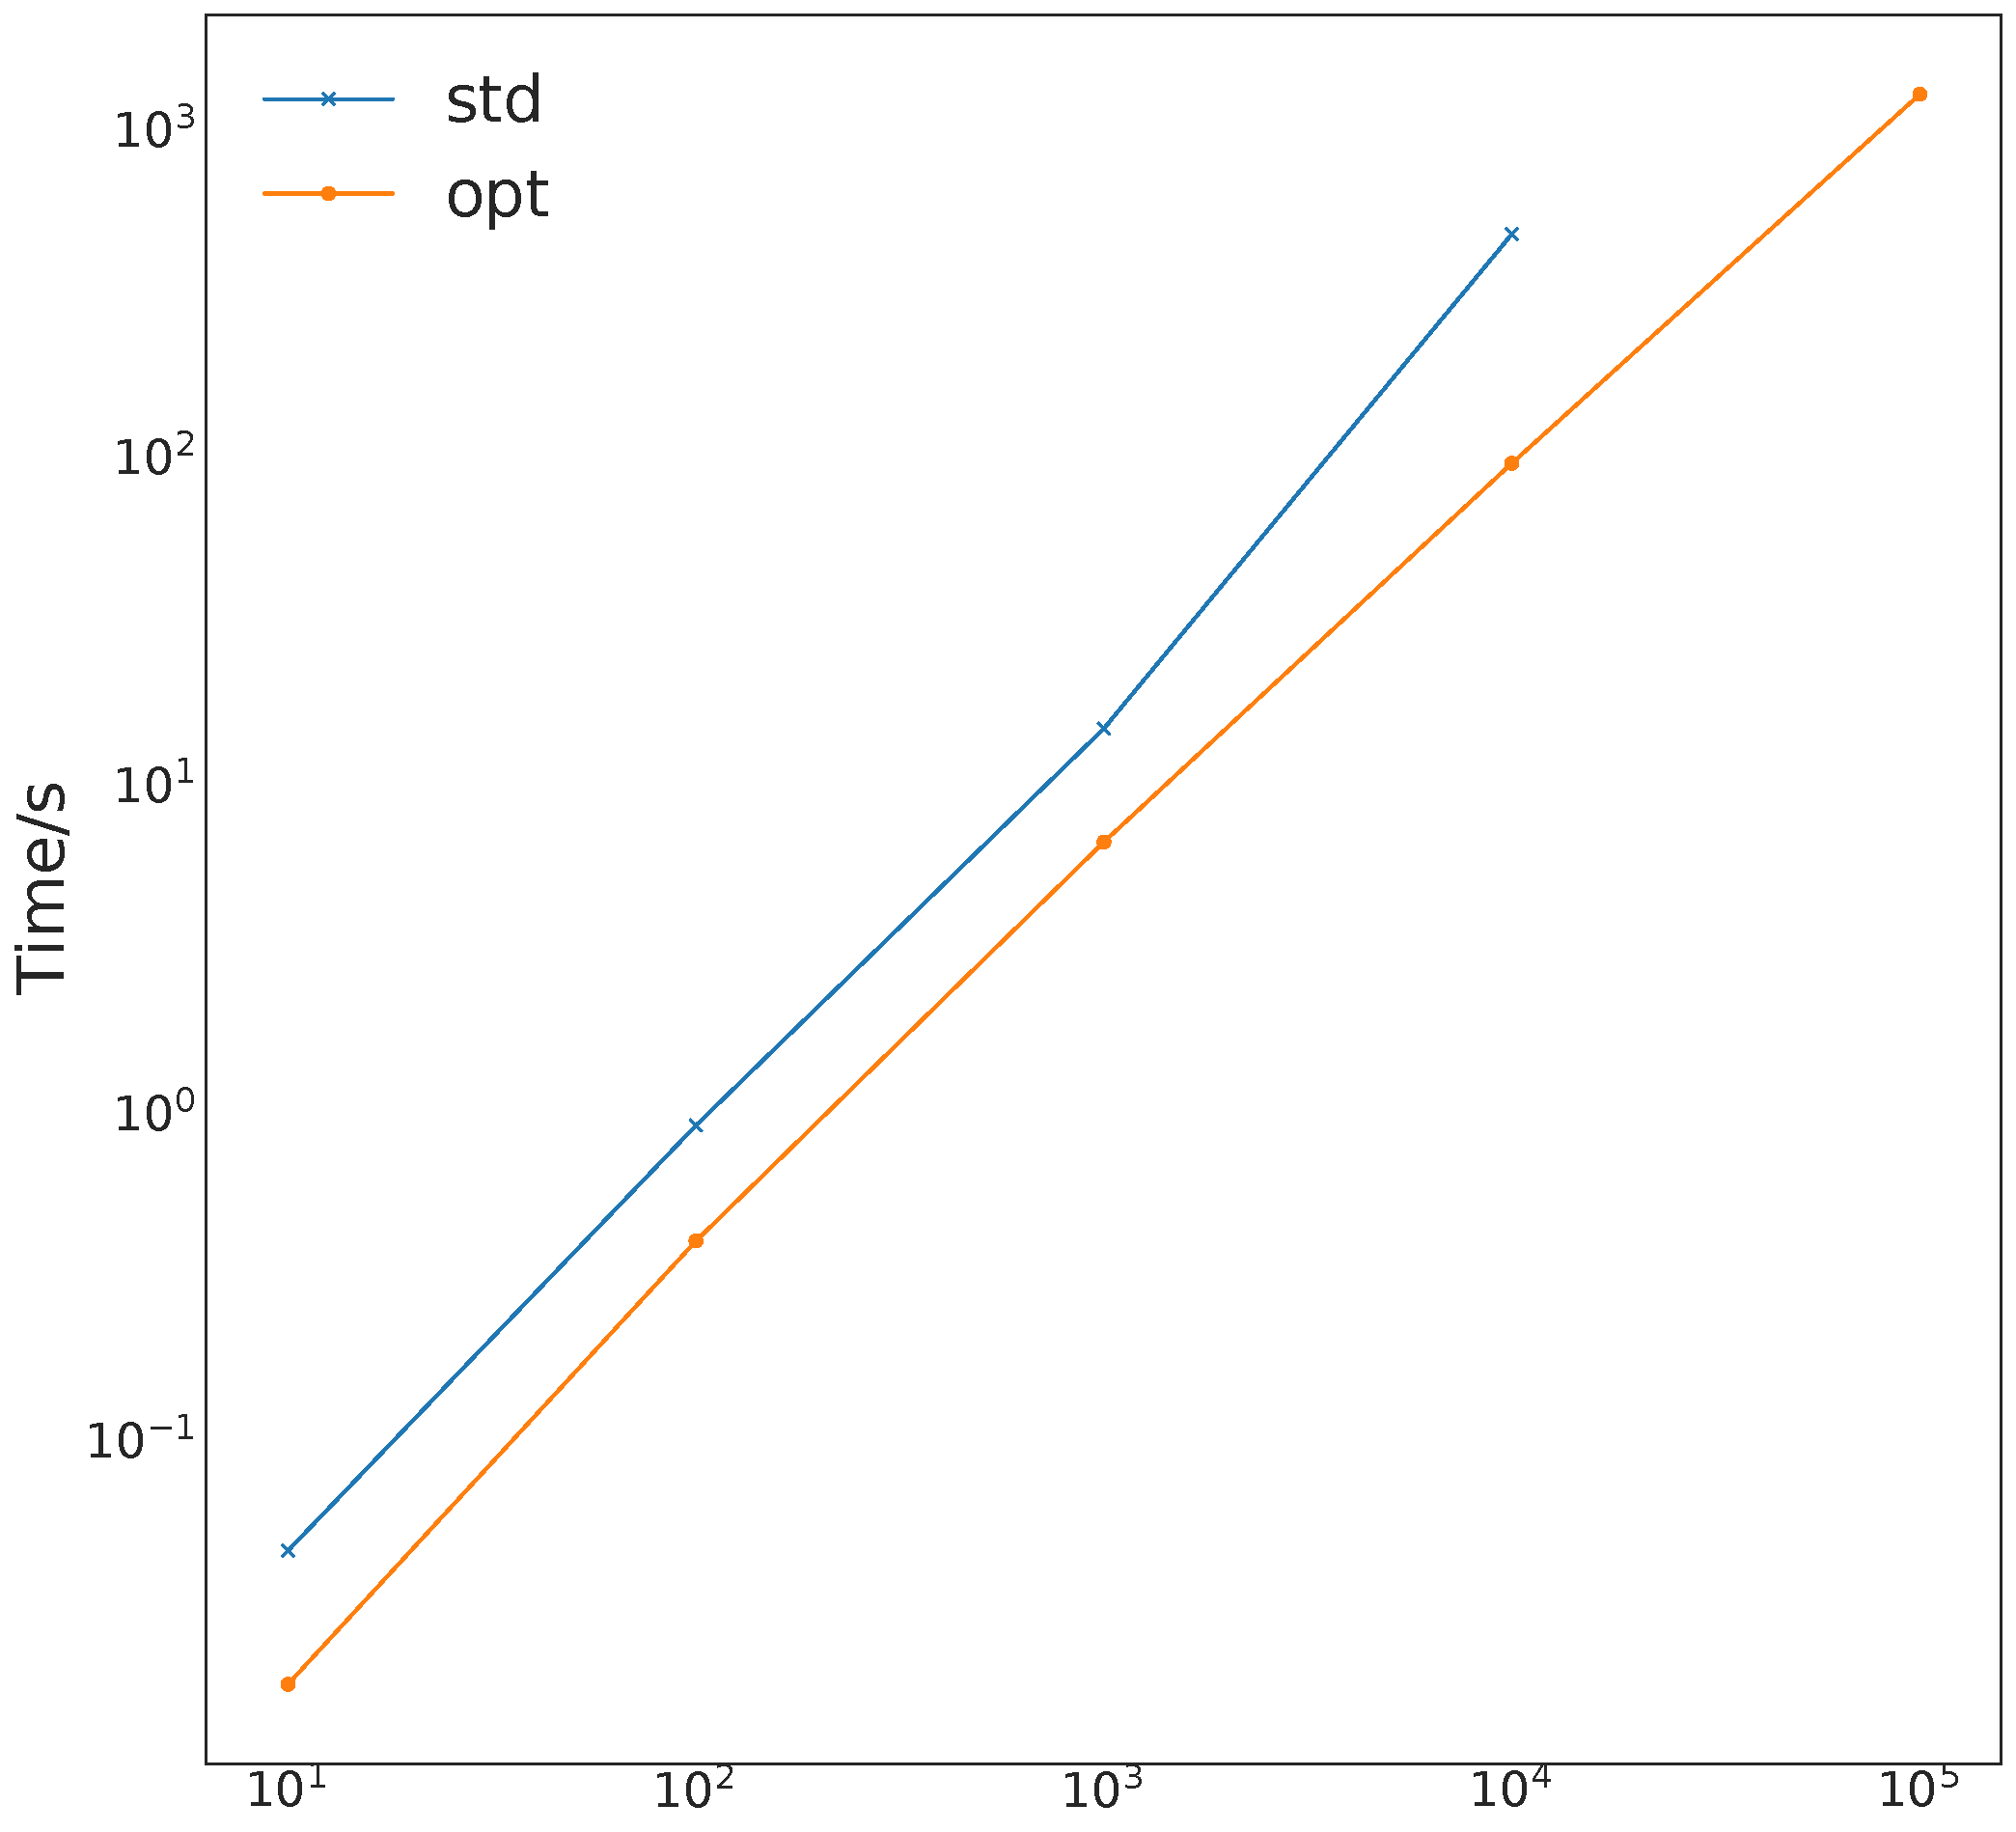
\includegraphics[scale=0.15]{img/ss-sorting.pdf}
    \caption{Performance of sorting in Shamir's secret sharing protocol}
    \label{sssorting}
\end{figure}
In Shamir's secret sharing protocol, our opt program achieves 5.0$\times$ speedup, as shown in Fig. \ref{sssorting}.
\begin{figure}[h]
    \centering
    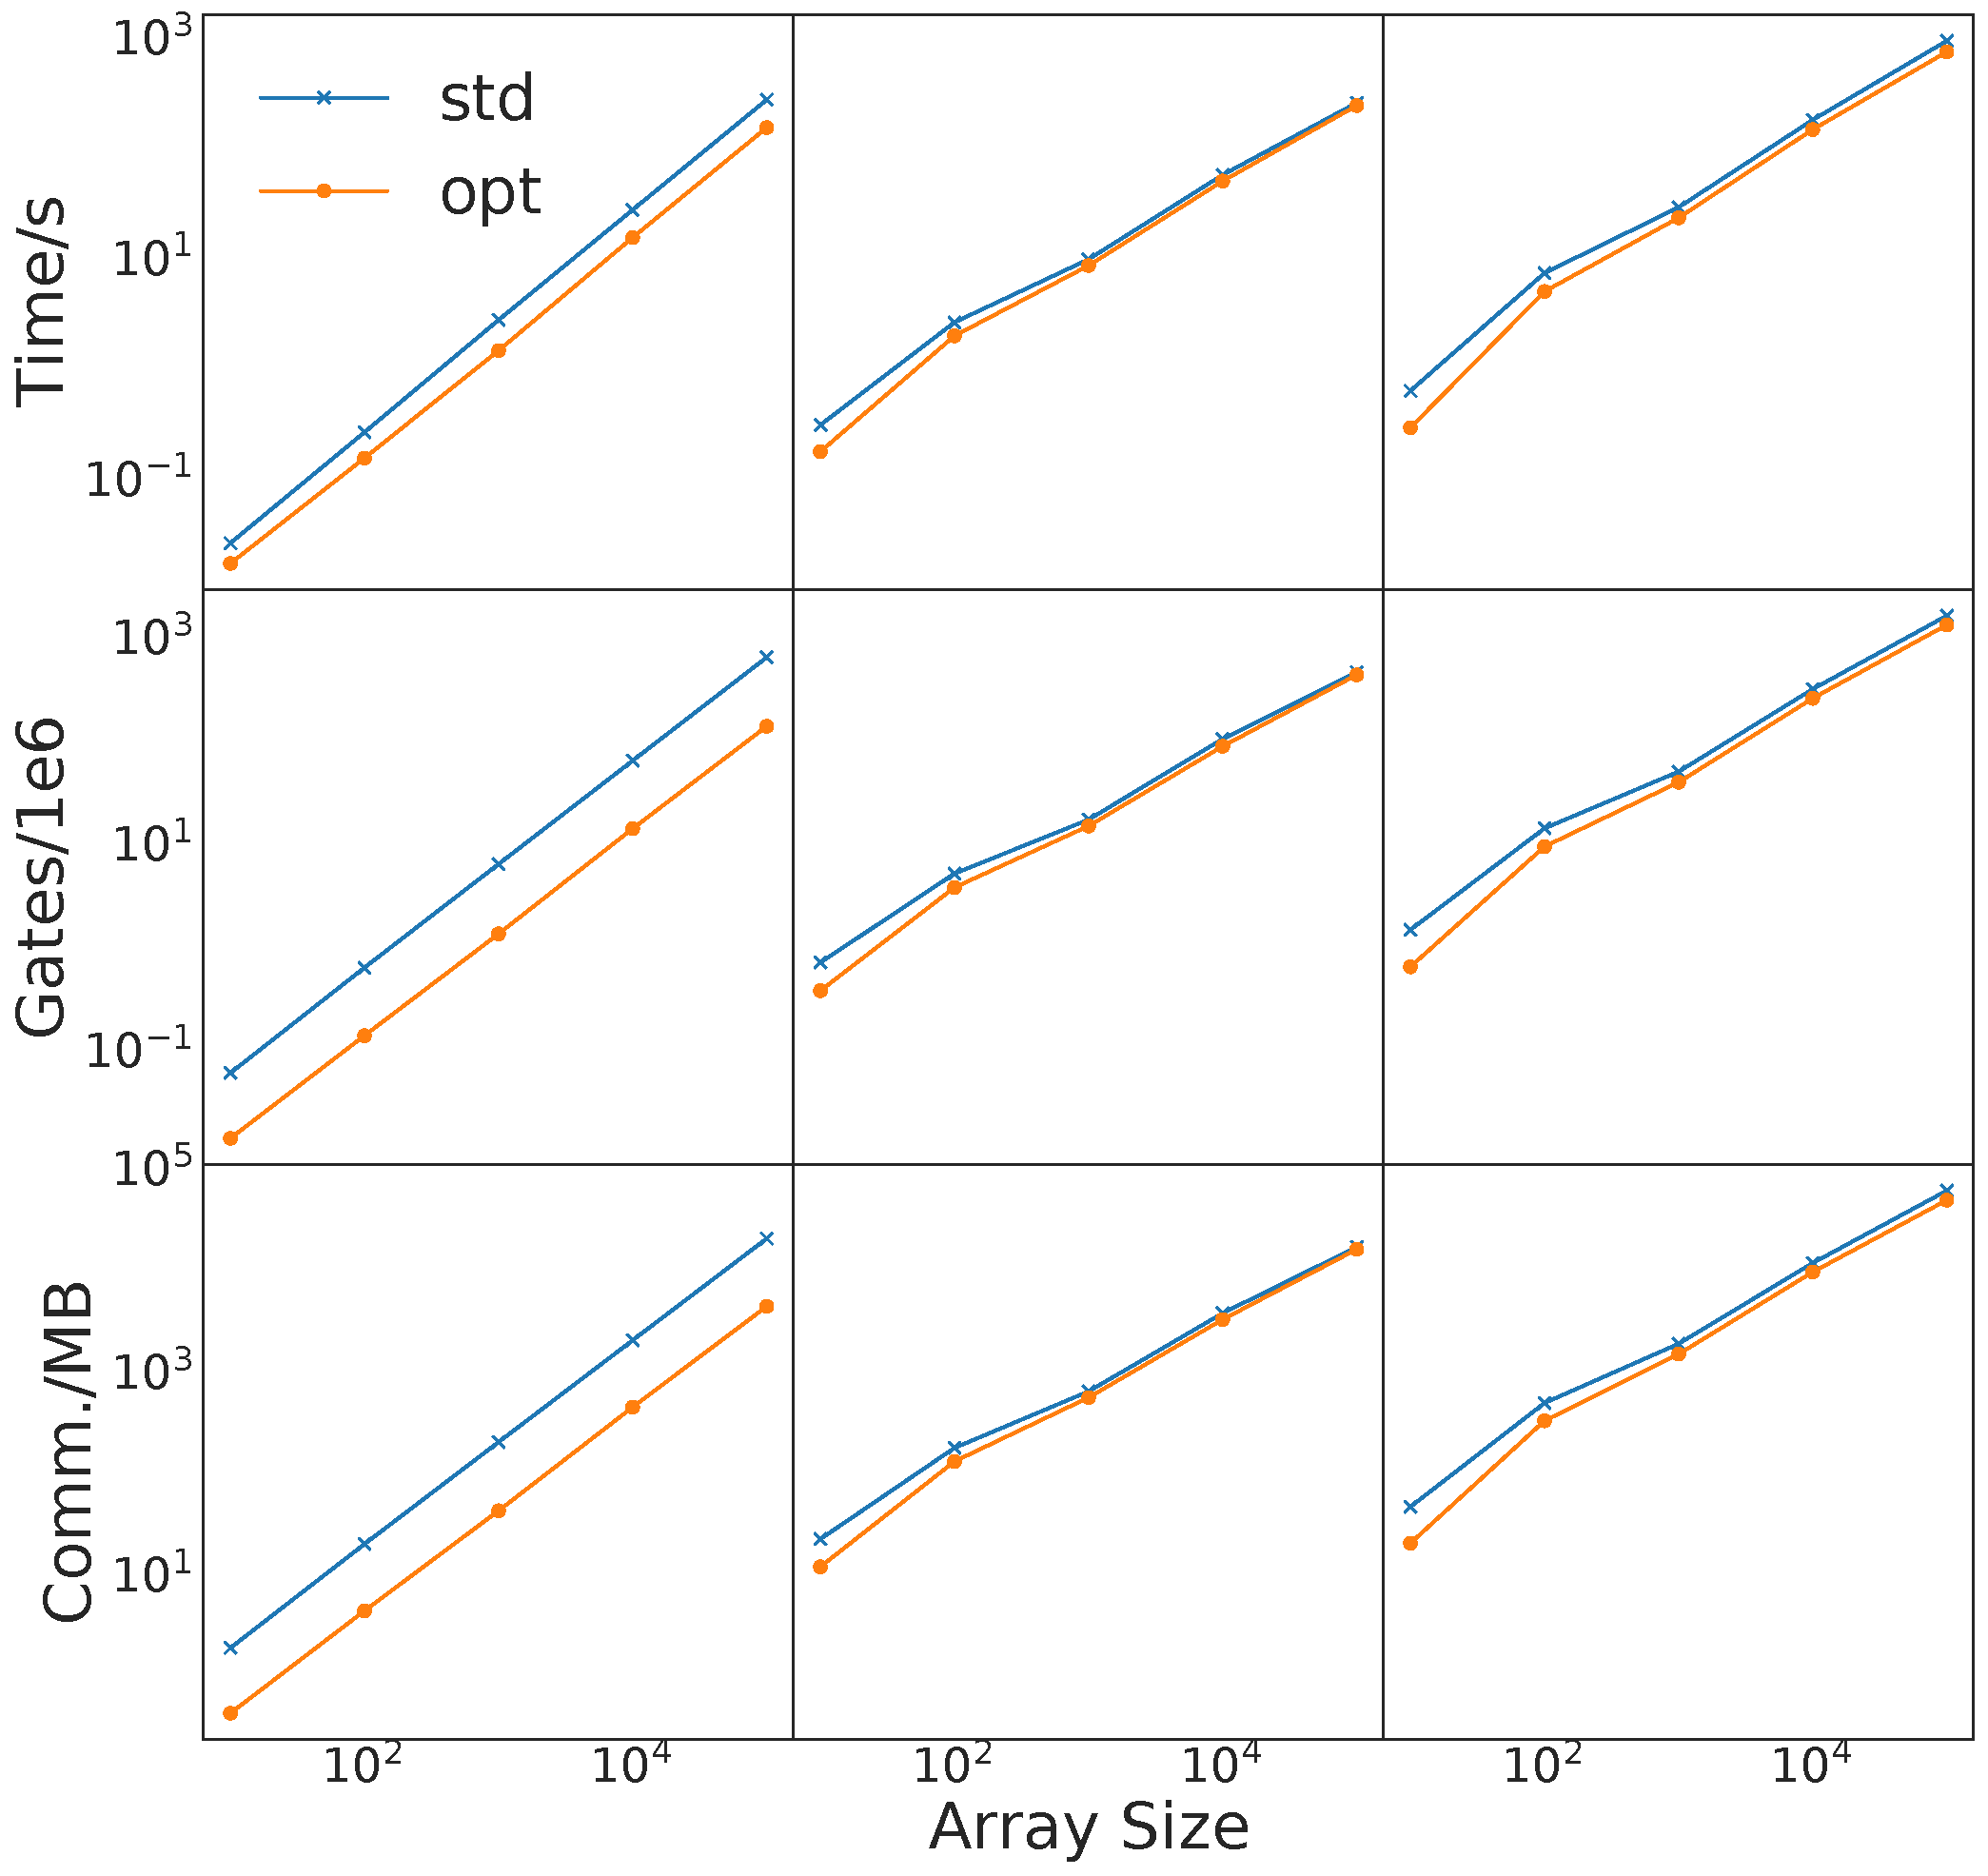
\includegraphics[scale=0.2]{img/gc-search.pdf}
    \caption{Performance of Linear (left), Binary (mid), Almost Search (right) in Yao's garbled circuit protocol}
    \label{gcsearch}
\end{figure}
Our optimization strategy is suitable for different MPC protocols.
From the experiment result, our opt program improves the performance both in Yao's garbled circuit protocol and Secret Sharing protocol.

In this case, the MPC Batcher sort algorithm has $O(n\log^2{n})$ average  time complexity.
With appropriate optimization of the MPC quick sort algorithm, our opt program has  $O(n\log{n})$ average time complexity.
The opt program performs better as the inputs scale increase.

Fig. \ref{gcsearch} shows the performance of three different search study cases in Yao's garbled circuit protocol.
The measurement is searching 100 random elements in the same array.
As array size increases, the performance of opt is reduced because the array size is much larger than 100.
The opt performs better if it searches more elements.
However, our opt program reduces 78\% gates and communications and achieves 1.79$\times$ speedup for linear search.
Binary search work worse than linear search because binary search needs oblivious RAM to access item with secret index.
\begin{figure}[h]
    \centering
    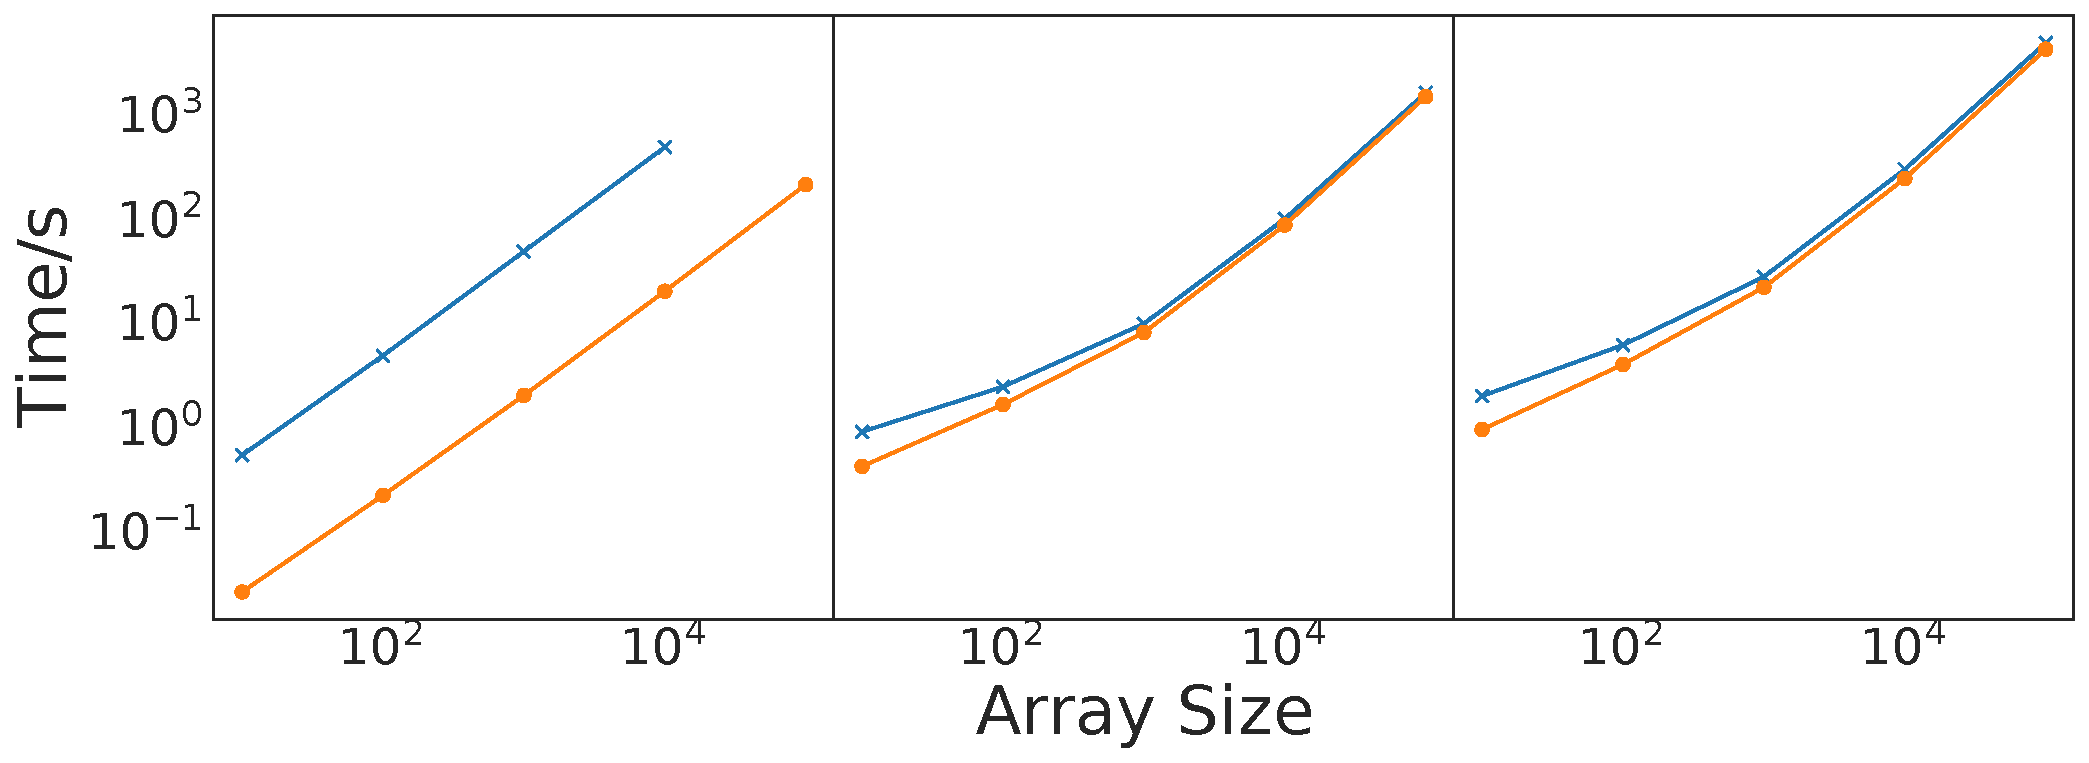
\includegraphics[scale=0.2]{img/ss-search.pdf}
    \caption{Performance of Linear (left), Binary (mid), Almost Search (right) in Shamir's secret sharing protocol}
    \label{sssearch}
\end{figure}
Fig. \ref{sssearch} shows the performance of search study cases in Shamir's secret sharing protocol.
Our opt linear search achieves 24.14$\times$ speedup in 10k array size.
Opt binary search and almost search achieves 1.48$\times$ and 1.54$\times$ speedup when the array size is equal to search size.
The difference of improvement can be explained that Shamir's secret sharing protocol performs not well on comparison operations and oblivious RAM is expensive.

In Yao's garbled circuit protocol, the opt program of line segments intersection reduces 20\% gates and communications and achieves 1.25$\times$ speedup by avoiding calculating coordinates when line segments do not intersect.
The opt program of PSI reduces about 73\% gates and communications and achieves 1.5$\times$ speedup.
In Shamir's secret sharing protocol, the speedup of line intersection and PSI is 1.25$\times$ and 15$\times$.




% \begin{table*}[t]
% \centering
% \setlength{\tabcolsep}{1mm}
% \caption{Execution Time/s of Benchmarks on Garbled Circuit Protocol}
% \begin{tabular}{c|ccccc|ccccc|ccccc}
% \hline
% \multirow{2}{*}{Name} & \multicolumn{5}{c|}{std's input size}       & \multicolumn{5}{c|}{opt's input size}       & \multicolumn{5}{c}{improvement}     \\ \cline{2-16}
%                       & 10    & 100   & 1,000  & 10,000   & 100,000 & 10    & 100   & 1000   & 10000    & 100000  & 10   & 100  & 1000 & 10000 & 100000 \\ \hline
% Sort                  & 0.002 & 0.051 & 0.990  & 18.668   & 295.548 & 0.001 & 0.027 & 0.394  & 5.500    & 77.019  & 50\% & 47\% & 60\% & 71\%  & 74\%   \\ \hline
% Linear Search         & 0.026 & 0.262 & 2.724  & 27.080   & 269.210 & 0.017 & 0.153 & 1.441  & 15.203   & 150.606 & 35\% & 42\% & 47\% & 44\%  & 44\%   \\ \hline
% Binary Search         & 0.305 & 2.595 & 9.662  & 56.205   & 252.489 & 0.175 & 1.958 & 8.477  & 49.390   & 238.511 & 43\% & 25\% & 12\% & 12\%  & 6\%    \\ \hline
% Almost Search         & 0.623 & 7.248 & 28.576 & 176.673  & 919.378 & 0.288 & 4.937 & 22.954 & 144.593  & 729.812 & 54\% & 32\% & 20\% & 18\%  & 21\%   \\ \hline
% Quadratic PSI         & 0.003 & 0.264 & 26.514 & 2647.793 & /       & 0.002 & 0.182 & 17.700 & 1865.526 & /       & 33\% & 31\% & 33\% & 30\%  & /      \\ \hline
% Line Intersection     & 0.284 & 2.642 & 28.723 & 267.920  & /       & 0.216 & 2.273 & 23.350 & 212.480  & /       & 24\% & 14\% & 19\% & 21\%  & /      \\ \hline
% \end{tabular}
% \label{tabgc}%
% \end{table*}

% \begin{table*}[t]
% \centering
% \setlength{\tabcolsep}{1mm}
% \caption{Execution Time/s of Benchmarks on Secret Sharing Protocol}
% \begin{tabular}{c|ccccc|ccccc|ccccc}
% \hline
% \multirow{2}{*}{Name} & \multicolumn{5}{c|}{std's input size}         & \multicolumn{5}{c|}{opt's input size}          & \multicolumn{5}{c}{improvement}     \\ \cline{2-16}
%                       & 10    & 100    & 1,000   & 10,000  & 100,000  & 10    & 100    & 1000    & 10000    & 100000   & 10   & 100  & 1000 & 10000 & 100000 \\ \hline
% Sort                  & 0.046 & 0.912  & 14.817  & 477.358 & /        & 0.018 & 0.405  & 6.677   & 95.459   & 1274.804 & 61\% & 56\% & 55\% & 80\%  & /      \\ \hline
% Linear Search         & 0.534 & 4.821  & 48.126  & 481.939 & /        & 0.026 & 0.220  & 2.001   & 19.966   & 210.700  & 95\% & 95\% & 96\% & 96\%  & /      \\ \hline
% Binary Search         & 0.896 & 2.425  & 9.754   & 99.043  & 1601.835 & 0.417 & 1.637  & 8.025   & 86.270   & 1470.157 & 53\% & 32\% & 18\% & 13\%  & 8\%    \\ \hline
% Almost Search         & 1.975 & 6.087  & 27.509  & 295.545 & 4823.228 & 0.941 & 3.960  & 21.802  & 240.973  & 4195.490 & 52\% & 35\% & 21\% & 18\%  & 13\%   \\ \hline
% Quadratic PSI         & 0.056 & 4.800  & 475.423 & /       & /        & 0.004 & 0.310  & 29.610  & 3216.808 & /        & 93\% & 94\% & 94\% & /     & /      \\ \hline
% Line Intersection     & 3.265 & 32.165 & 320.368 &         &          & 2.688 & 26.416 & 261.388 &          &          & 18\% & 18\% & 18\% & /     & /      \\ \hline
% \end{tabular}
% \label{tabss}%
% \end{table*}

\end{comment}

\section{Related work}\label{sec:relatedwork}
% \subsection{Multi-party computation frameworks}
% Obliv-C\cite{oblivc}  is a simple GCC wrapper that makes embedding secure computing protocols in regular C programs. Obliv-C implements Yao's GC protocol and provides programmers a flexible control to the program executions. The Obliv-C compiler transforms an Obliv-C language program into a secure multi-party encryption protocol. The protocol performs operations without revealing any input or computed intermediate values to either party. Only the final output will be displayed.

% MPyC\cite{mpyc} is a python library for MPC. It provides a python interface for fast prototyping and execution against the malicious adversary. MPyC implements Shamir's threshold secret sharing over finite fields, supports secure m-party computation.

% MP-SPDZ \cite{spdz20} features a python-based front end and implements a large set of schemes, including multi-party circuit-based, hybrid, and garbled circuit protocols.  MP-SPDZ implements MPC protocol variants that cover the most commonly used security models.  However, MP-SPDZ generates the whole circuit in the compilation process so that it can't dynamically generate circuits during the execution.

% ABY\cite{aby2}, EMP toolkit\cite{emp}, Frigate\cite{frigate16} and etc also perform secure computation. A recent SoK\cite{mpcsok} gives the survey and comparison of most MPC compilers.



\noindent
{\bf MPC Frameworks.}
Early efforts to MPC frameworks provide high-level languages for specifying MPC applications and compilers
for translating them into executable implementations~\cite{Fairplay04,Ben-DavidNP08,BogdanovLW08,DamgardGKN09,BurkhartSMD10,HolzerFKV12,SonghoriHS0K15,frigate16}.
For instance, Fairplay complies 2-party MPC programs written in a domain-specific language into
Yao's garbled circuits~\cite{Fairplay04}. FairplayMP~\cite{Ben-DavidNP08} extends
Fairplay to multi-party using a modified version of the BMR protocol~\cite{BeaverMR90} with a Java-language interface.
The others~\cite{BogdanovLW08,DamgardGKN09,BurkhartSMD10,HolzerFKV12,SonghoriHS0K15,frigate16}
are aimed to improve the efficiency of operations in circuits and size of circuits.
%Sharemind~\cite{BogdanovLW08}, VIFF~\cite{DamgardGKN09}, SEPIA~\cite{BurkhartSMD10}, CBMC-GC~\cite{HolzerFKV12}, TinyGarble~\cite{SonghoriHS0K15} and Frigate~\cite{frigate16}
%are proposed to improve the efficiency of operations in circuits and size of circuits.
Mixed MPC protocols were also proposed to improve efficiency~\cite{HeneckaKSSW10,SchropferKM11,BogdanovLR14,RastogiHH14,LaudR15,Demmler0Z15,MohasselR18,hycc18,aby221}, as the efficiency of MPC protocols vary in operations.
These frameworks explore the implementation space of operations in specific MPC protocols (e.g., garbled circuits, secret sharing
and homomorphic encryption), as well as their conversions.
%Among them, Wysteria~\cite{RastogiHH14}
%is the first work that formalizes operational semantics of its domain-specific language and proposes a refinement type system for reasoning about correctness.
However, all these frameworks either entirely compile an MPC program
or compile an MPC program according to user-annotated secret variables to improve performance, but without formal security guarantees.
Our approach improves the performance of MPC applications by declassifying secret variables without compromising security,
thus it is orthogonal to the above optimization works.


\smallskip
\noindent
{\bf Security of MPC applications.}
Since MPC applications implemented in MPC frameworks do not necessarily secure
due to information leakage during execution in the real-world. Therefore,
information-flow type systems and data flow analysis have been adopted in the MPC frameworks~\cite{NielsenS07,Mitchell0SZ12,picco13,LiuHSKH14,LiuWNHS15,ZahurE15,ChandranGRST19,MPyC20,spdz20}.
%EzPC~\cite{ChandranGRST19} SMCL~\cite{NielsenS07}, PICCO~\cite{picco13}, SCVM~\cite{LiuHSKH14}, ObliVM~\cite{LiuWNHS15}, Obliv-C~\cite{ZahurE15}, MPyC~\cite{MPyC20}, MP-SPDZ~\cite{spdz20},
%and the Haskell extension~\cite{Mitchell0SZ12}.
However, these works only consider security verification, instead of
automatically generation of security policies as we did.
Moreover,
these approaches cannot identify some variables (e.g., {\tt c2} in our motivating example)
that can be declassified without compromising security.
Kerschbaum~\cite{Kerschbaum11} proposed to infer public intermediate values
by reasoning about epistemic modal logic, similar goal to ours for declassifying secret variables.
However, it is unclear how efficient is this approach, as the performance of their approach was
not reported in~\cite{Kerschbaum11}.



Alternatively, self-composition  which reduces the security problem to
the safety problem on two copies of a program has been adopted by~\cite{RastogiMHH13,mpcleak18,RastogiSH19},
%\fan{\cite{,spdz20} are common frameworks,  didn't consider declassify variables and didn't provide program verification functionality. Remove them?}
where the safety problem can be solved by safety verification tools.
However, safety verification remains challenging and these approaches often require user annotations (e.g., procedure contracts and loop invariants) that are non-trivial for MPC practitioners. %and users
%often have to annotate loop invariants, while writing
%useful loop invariants is non-trivial for MPC developers.
Compared over these works,
there are three differences:
(1) they only use the self-composition reduction to verify security instead of automatically generating a security policy;
(2) they have to check almost all the program variables which is computational expensive,
 while we first apply an efficient type system to infer a security policy
and then only check if the security branching variables in the security policy
can be declassified;
and (3) we check if security branching variables can be declassified by reasoning about pairs of symbolic executions which can be seen as a divide-and-conquer approach
without annotations and the results are fed back to the type system to efficiently refine security levels.
We also remark that the self-composition reduction could also be used to check if a security branching variable
could be declassified.




%TASTY~\cite{HeneckaKSSW10} combines homomorphic encryption
%with Yao's garbled circuits. L1~\cite{SchropferKM11} proposes a language for specifying mixed protocols.
%Sharemind is extended mixed protocols~\cite{BogdanovLR14,LaudR15}.
% ABY~\cite{Demmler0Z15} ABY2.0~\cite{aby221}, ABY$^3$~\cite{MohasselR18}, HyCC~\cite{hycc18},

 %EMP-toolkit~\cite{emp-toolkit16},



\smallskip
\noindent
{\bf Information-flow analysis.}
A rich body of literature has studied the verification of information-flow security and noninterference
in programs~\cite{DenningD77,GoguenM82a}, which requires that confidential data does not flow to
outputs. This is too restrictive for programs which allows secret data to flow to some non-secret outputs, e.g.,
MPC applications, therefore the security notion is extended with declassification (a.k.a. delimited release) later~\cite{LiZ05,SabelfeldS09}.
These security problems are verified by type systems (e.g.~\cite{VolpanoIS96,SabelfeldM03,LiZ05}) or
self-composition (e.g.,~\cite{TerauchiA05,BartheDR11}) or relational reasoning~(e.g.,~\cite{AmtoftBB06,SousaD16,BartheCK11}).
Some of these techniques have been adapted to verify timing side-channel security, e.g.,~\cite{AlmeidaBBDE16,ChenFD17,YangVSGM18,CauligiSJBWRGBJ19}.
However, the usual notions of security in these settings do not require reasoning about arbitrary leakage
and these works are not directly applicable to our setting, although some of those techniques have been adapted to verify
security of MPC applications.




\begin{comment}

\subsection{Trade-off between performance and privacy}
Almeida et al. and  Fischer et al. study the tradeoff between performance and privacy for privacy-preserving computation in recent years.
Both work \cite{mpcleak18,pasapto} consider revealing information about private data to improve performance.
\cite{mpcleak18} allows a semantic leakage upper bound and uses Boogie verification toolchain to verify whether the leakage of a program is beyond the given upper bound.
The programmer gives the upper bound and writes annotations including precondition, postcondition, and loop invariants into source code to guide the theorem prover to complete the verification.
The verification conditions heavily rely on the knowledge of programmers.

\cite{pasapto} quantizes the information leakage of private inputs as the number of bits.
It models the tradeoff as an optimization problem.
\cite{pasapto} heuristically searches the variants which reveal some privacy information flow of the program to find an optimal variant within a user given leakage upper bound.

\subsection{Circuit level optimization}
Circuit level optimization reduces gate cost for general MPC.
The state-of-the-art circuit level optimization technique is Half Gates \cite{halfgate} which leverages prior optimization work \cite{BeaverMR90,grr3,freexor}.
Half Gates divides an AND gate into two half gates, one for garbler and the other one for evaluator.
Half Gates needs two ciphertexts in communications for an AND gate while the classical gates need eight ciphertexts.
Half Gates needs no communications for XOR gates that are compatible with Free XOR \cite{freexor}.

\subsection{Specified protocol}
For MPC problems with important applications, researchers always design specified protocols to achieve higher performance than general protocols.
For example, the Private Set Intersection (PSI) problem.

Pinkas et al. \cite{pssz} design a two-party PSI protocol using permutation-based hashing.
The performance of \cite{pssz} is much better than circuit-based PSI and OT-based PSI
\cite{pssz} achieves 3$\times$-4$\times$ overhead than insecure hashing PSI protocol for 32-bit item length and sufficiently large sets.

Kolesnikov et al. \cite{kol} proposed the state-of-the-art PSI protocol based on \cite{pssz} with an efficient OPRF.
\cite{kol} achieves about 3$\times$ speedup than \cite{pssz} for 128 bit item length and sufficiently large sets.

\subsection{Hybrid protocol}
ABY \cite{aby221} is a hybrid protocol framework for two-party MPC.
ABY provides switches among Arithmetic GMW protocol,  Boolean GMW protocol, and Yao's garbled circuit protocol.
Programmers can assign different protocols to different computations to achieve higher performance.
For example, computing arithmetic operations using Arithmetic GMW protocol and computing comparison operations using Yao's garbled circuit protocol.

HyCC \cite{hycc18} proposes the protocol selection for hybird protocol.
HyCC splits the full functionality into small parts.
In the protocol selection phase, HyCC benchmarks the cost of each operation and decides the protocol for each small part by optimizing a cost function.
ABY \cite{aby221} assigns protocol to operations during the development process.
The assignment relies on the knowledge of programmers.
But HyCC \cite{hycc18} selects protocol according to the running environment.
\end{comment}


\section{Conclusion}\label{sec:conclusion}
We have formalized the leakage of an MPC application %as a set of private inputs
bridging the language-level and protocol-level leakages
via security policies. Based on the formalization,
we have presented an approach to automatically synthesize a security policy
%that declare as few secret variables as possible but
which can improve the performance of the MPC applications while not compromising their privacy.
Our approach is essentially a synergistic integration of type inference and
symbolic reasoning with security type refinement.
We implemented our approach in a tool \TNAME.
The experimental results on five typical MPC applications confirm
that our approach can significantly improve
the performance of MPC applications.


%%%%%%%%%%%%%%%%%%%%%%%%%%%%%%%%%%%%%%%%%%%%%%%%%%%%%%%%%%%%%%%%%%%%%%%%%%%%%%%%%%%%%%%%
\newpage
\bibliographystyle{splncs04}
\bibliography{mpc}
%%%%%%%%%%%%%%%%%%%%%%%%%%%%%%%%%%%%%%%%%%%%%%%%%%%%%%%%%%%%%%%%%%%%%%%%%%%%%%%%%%%%%%%%%
\newpage
\appendix
\section{Appendix}\label{sec:appendix}

\subsection{MPC Protocols}\label{sec:protocols}
In general, there are three fundamental protocols to achieve semi-honest security:
garbled circuits~\cite{yao82,freexor,BeaverMR90}, secret sharing~\cite{Shamir79,GMW}, and homomorphic encryption~\cite{SHE},
varying in their computational, circuit and communication complexity.

\smallskip
\noindent
{\bf Garbled circuits}. The garbled circuit protocol was proposed by Yao for 2-party MPC.
Roughly speaking,
one party (say $\Party{1}$) encodes
the computation $f(x_1,x_2)$ as a Boolean circuit $C$, then garbles it.
The garbling procedure uses two random keys to denote the truth values of each wire
and symmetric-key encrypts the circuit $C$, ensuring that learning one random key for each fan-in allows to decrypt exactly one output of fan-out for each gate.
Next, $\Party{1}$ sends the garbled circuit, random keys of the truth values of $\Party{1}$'s private inputs,
and all the random keys of $\Party{2}$'s private inputs
to $\Party{2}$. %For each private input of the participant $\Party{2}$,
$\Party{2}$ chooses the random keys of the truth values of her private inputs and evaluates the garbled circuit %$GC$ %using the random keys of the inputs
%of both participants
by performing symmetric-key decryption. % for every gate.
%Recall that using one random key per input allows $\Party{2}$ to decrypt exactly one row of its garbled
%truth-table.
After successfully decrypting all the gates, $\Party{2}$ obtains the result of the garbled circuit
and sends it back to $\Party{1}$, from which $\Party{1}$ can obtain the result $f(x_1,x_2)$ and reveals
it to $\Party{2}$. To be semi-honest secure,
%for each his/her private input,
$\Party{2}$ is enforced to choose only one random key per $\Party{2}$'s private input and does not know the another random key, moreover, $\Party{1}$ does not know which random key
was chosen by  $\Party{2}$.
%This requirement is achieved via oblivious transfer~\cite{EvenGL85}.
%During the execution of the protocol, both participants only send and receive random keys,
%except for the final result $f(x_1,x_2)$.
%Thus, it is semi-honest secure.
Yao's garbled circuit protocol has been extended to multi-party MPC
with a distributed garbling procedure~\cite{BeaverMR90}.


\smallskip
\noindent
{\bf Secret sharing}. For an MPC application $f(\vec{x}_n)$, an $(n,t)$-secret sharing scheme   splits the private input $x_i$ of each party $\Party{i}$
into $n$ shares using random values and sends $n-1$ shares to the other parties, one share per party.
Any $t-1$ shares of the private input $x_i$ reveal no information of the private input $x_i$.
The computation $f(\vec{x}_n)$  is transformed into a Boolean or arithmetic circuit $C$ according to the secret sharing scheme
such that each party evaluates the circuit $C$ using the received shares from the other parties.
The results of the circuit $C$ of all the parties form
the share of the desired result $f(\vec{x}_n)$, from which
each party can reconstruct the result $f(\vec{x}_n)$.
For instance, using the Boolean secret sharing scheme, $x_i$ can be split into
the shares $(x_i^1,\cdots,x_i^n)$, where $x_i^1,\cdots,x_i^{n-1}$ are uniformly sampled
random values, $x_i^n=x_i^1\oplus \cdots\oplus x_i^{n-1}$ is the exclude-or of $x_i^1,\cdots,x_i^{n-1}$.
Using the additive secret sharing scheme, an element $x_i$ of a finite field can be split into
the shares $(x_i^1,\cdots,x_i^n)$,  $x_i^1,\cdots,x_i^{n-1}$ are uniformly sampled
random values from a finite field, $x_i^n=x_i^1+ \cdots+ x_i^{n-1}$, where $+$ is the finite field addition operation.

\medskip
\noindent
{\bf Homomorphic encryption}.
Homomorphic encryption enables computations on ciphertexts to compute
an encrypted result that, when decrypted, is the result $f(\vec{x}_n)$.
For instance, to compute an MPC application $f(\vec{x}_n)$,
all the parties encrypt their private inputs using the same public key
and then send the encrypted inputs to an untrusted third party.
The untrusted third party computes the encrypted result of $f(\vec{x}_n)$
using the encrypted inputs and sends the result back to the parties.
Finally, each party can obtain the result $f(\vec{x}_n)$ by decrypting
the encrypted result.

%The above three fundamental protocols are the base protocols for today's MPC.

%
%
%Yao firstly introduced the MPC problem in the early 1980s \cite{EvansKR18}.
%In \cite{yao82}, Yao proposed Yao's garbled circuit protocol for solving the MPC problem.
%Goldreich et al. \cite{GMW} proposed an additive secret sharing approach to solve MPC.
%A decade ago, Damg{\aa}rd et al. \cite{SHE} proposed a new MPC approach based on %a somewhat
%homomorphic cryptosystems.
%The above three protocols and their ideas became the basis of research work in the field of MPC protocol design.
%Garbled circuits, secret sharing, and homomorphic encryption have become the base protocols for today's MPC implementations.
%Due to the unresolved performance issues of homomorphic encryption, real-world MPC implementations tend to choose either garbled circuit-based protocols or secret-sharing-based protocols.
%In the experiment section, we consider experiments on the implementation of these two protocols.



\subsection{The Operational Semantics of {\LANG} Programs}
\label{sec:semantics}
The operational semantics of {\LANG} programs is shown in Fig.~\ref{fig:semantics}.
\begin{figure}[t]
    \centering
\scalebox{0.9}{
    \begin{tabular}{cc}
%    \hline\specialrule{0em}{3pt}{3pt}
%%%%%%%%%%%%%%%%%%%%%%%%%%%%%%%%%%%%%%%%%%
    $\begin{array}{c}
     \hline
        \MPCAngle{x=e, \sigma} \rightarrow \MPCAngle{{\Pskip}, \sigma[x\mapsto  \sigma(e)]}
    \end{array}$ &
%%%%%%%%%%%%%%%%%%%%%%%%%%%%%%%%%%%%%%%%%%
        $\begin{array}{c}
      %  \MPCState{e}{\sigma}=v \\
     \hline
        \MPCAngle{{\Preturn} \ x, \sigma} \rightarrow \MPCAngle{{\Pskip}, \sigma}
    \end{array}$ \\ \\
%%%%%%%%%%%%%%%%%%%%%%%%%%%%%%%%%%%%%%%%%%
   $\begin{array}{c}
        \MPCAngle{p_{1}, \sigma_{1}}             \rightarrow      \MPCAngle{ {\Pskip}, \sigma_{2} } \quad
        \MPCAngle{p_{2}, \sigma_{2}}    \rightarrow   \MPCAngle{ p_{2}' , \sigma_{3} } \\
        \hline
        \MPCAngle{p_{1};p_{2}, \sigma_{1}}       \rightarrow   \MPCAngle{p_{2}', \sigma_{3}}
    \end{array}$ \qquad\qquad&
%%%%%%%%%%%%%%%%%%%%%%%%%%%%%%%%%%%%%%%%%%
    $\begin{array}{c}
        \MPCAngle{p_1,\sigma_{1}}    \rightarrow    \MPCAngle{ p_1', \sigma_{2}}    \quad     p_{1}' \neq {\Pskip} \\
        \hline
        \MPCAngle{p_{1} ; p_{2}, \sigma_{1}} \rightarrow \MPCAngle{p_1^{\prime};p_2, \sigma_{2}}
    \end{array}$  \\ \\
%%%%%%%%%%%%%%%%%%%%%%%%%%%%%%%%%%%%%%%%%%
 $\begin{array}{c}
        p= \sigma(x) \ ? \ p_1 : \ p_2 \\
        \hline
        \MPCAngle{{\Pif} \ x \ {\Pthen} \  p_1 \ {\Pelse} \ p_2, \sigma}   \rightarrow  \MPCAngle{p,\sigma}
    \end{array} $ &
%%%%%%%%%%%%%%%%%%%%%%%%%%%%%%%%%%%%%%%%%%
   $ \begin{array}{c}
        p'=\sigma(x) \ ? \ p;{\Pwhile} \ x \ \Pdo \ p \ : \ {\Pskip} \\
        \hline
        \MPCAngle{{\Pwhile} \ x \ \Pdo \ p, \sigma}\rightarrow  \MPCAngle{p',\sigma}
    \end{array}$ \\ \\
%%%%%%%%%%%%%%%%%%%%%%%%%%%%%%%%%%%%%%%%%%
\multicolumn{2}{c}{$\begin{array}{c}
      p'= ( n\geq 1) \ ? \ p;{\Prepeat} \ n-1 \ \Pdo \ p \ : \ {\Pskip} \\
        \hline
        \MPCAngle{{\Prepeat} \ n \ \Pdo \ p, \sigma}\rightarrow  \MPCAngle{p',\sigma}
    \end{array}$ }\\ 
    \specialrule{0em}{3pt}{3pt}\hline
    \end{tabular}}
    \caption{The operational semantics of {\LANG} programs}
    \label{fig:semantics}
    % instrumented semantics
\end{figure}

\subsection{Proof of Proposition~\ref{prop:NI2Sec}}
{\bf Proposition~\ref{prop:NI2Sec}.}
\textit{If $p$ is $\varrho$-noninterfering for a security policy $\varrho$, then $\varrho\models_p f(\vec{x})$.}
%$\varrho$ is secure for the MPC application $f(x_1,\cdots, x_n)$
%whose functionality is implemented in $p$.



\begin{proof}
Assume the program $p$ is $\varrho$-noninterfering.
Consider the adversary-chosen  private inputs $\vec{v}_k\in\Dom^k$ for a constant $k\geq 1$, a result $v\in\Rng$ and a state $\sigma\in\leak_{\tt iw}^p(v,\vec{v}_k)$.
Let $\MPCAngle{\widehat{p}_\varrho,\sigma}\Downarrow \sigma_1:v$ be the execution
of $p$ starting from the state $\sigma$.
It suffices to show that $\leak_{\tt iw}^p(v,\vec{v}_k)\subseteq\leak_{\tt rw}^{p,\varrho}(v,\sigma)$,
as $\leak_{\tt iw}^p(v,\vec{v}_k)\supseteq\leak_{\tt rw}^{p,\varrho}(v,\sigma)$ always holds.
We show that $\sigma'\in\leak_{\tt rw}^{p,\varrho}(v,\sigma)$ for every $\sigma'\in\leak_{\tt iw}^p(v,\vec{v}_k)$.

Fix a state $\sigma'\in\leak_{\tt iw}^p(v,\vec{v}_k)$.
Let $\MPCAngle{\widehat{p}_\varrho,\sigma'}\Downarrow \sigma_1':v'$
be the execution of $p$ starting from the state $\sigma'$.
From $\sigma'\in\leak_{\tt iw}^p(v,\vec{v}_k)$, we get that $v'=v$.
Since $p$ is $\varrho$-noninterfering, we get that $\MPCAngle{\widehat{p}_\varrho,\sigma}\Downarrow_\varrho^{\Pub} \sigma_1:v$ and $\MPCAngle{\widehat{p}_\varrho,\sigma'}\Downarrow_\varrho^{\Pub} \sigma_1':v$
are the same. Therefore, $\sigma'\in\leak_{\tt rw}^{p,\varrho}(v,\sigma)$.\qed
\end{proof}




\subsection{Proof of Proposition~\ref{prop:symbleakage2}}
{\bf Proposition~\ref{prop:symbleakage2}.}
\textit{For each pair of
states $\sigma,\sigma'\in\leak_{\tt iw}^p(v,\vec{v}_k)$ such that
$\sigma\models \phi\wedge e=v$ and $\sigma'\models \phi'\wedge e'=v$,
if $\Psi_x(t,t')$ is valid and $\RW_{\varrho,\sigma}^{\Pub}(t)$ and $\RW_{\varrho,\sigma'}^{\Pub}(t')$ are identical,
then $\RW_{\varrho',\sigma}^{\Pub}(t)$ and $\RW_{\varrho',\sigma'}^{\Pub}(t')$ are identical,
where $\varrho'=\varrho[x\mapsto \Pub]$.}


\begin{proof}
Consider a pair of 
states $\sigma,\sigma'\in\leak_{\tt iw}^p(v,\vec{v}_k)$ such that
$\sigma\models \phi\wedge e=v$ and $\sigma'\models \phi'\wedge e'=v$.
Suppose $\RW_{\varrho,\sigma}^{\Pub}(t)$ and $\RW_{\varrho,\sigma'}^{\Pub}(t')$ are identical.
%Let $p_1,\cdots,p_m$ be the subsequence of the statements that are ${\Pif} \ x \ {\Pthen} \  p' \ {\Pelse} \ p''$ in $t$ and $t'$.
%Let $e_1,\cdots,e_m$ (resp. $e_1',\cdots,e_m'$) be symbolic values of $x$
%when executing $p_1,\cdots,p_m$ in the symbolic execution $t$ (resp. $t'$).


Let $\Primed(\sigma')$ be the state such that for every private input variable $x_i$,
$\Primed(\sigma')(x_i')=\sigma'(x_i)$.
Then, the model $(\sigma,\Primed(\sigma'))$ satisfies the constraint $\phi\wedge \Primed(\phi')\wedge e=\Primed(e')$.
Since $\Psi_x(t,t')$ is valid, the model $(\sigma,\Primed(\sigma'))$ also satisfies the constraint $\big(\bigwedge_{i=1}^m e_i=\Primed(e_i')\big)$.
This implies that once the same conditional statement $p_i$ is executed in $\RW_{\varrho,\sigma}(t)$ and $\RW_{\varrho,\sigma'}(t')$, they enter the same branch.
Therefore, $\RW_{\varrho',\sigma}^{\Pub}(t)$ and $\RW_{\varrho',\sigma'}^{\Pub}(t')$ are identical.
\qed
\end{proof}

\subsection{Proof of Theorem~\ref{thm:mainresult}}
{\bf Theorem~\ref{thm:mainresult}.}
\textit{If $\varrho\models_p f(\vec{x})$ and $\Psi_x(t,t')$ is valid for each pair of symbolic executions $t,t'\in\SymExe$ %such that ${\tt Stmt}_{\widehat{p}_\varrho}(t)$
%and ${\tt Stmt}_{\widehat{p}_\varrho}(t')$ are identical,
then, $\varrho[x\mapsto \Pub]\models_p f(\vec{x})$.}


\begin{proof}
Suppose $\varrho\models_p f(\vec{x})$. Then $\Enc_\varrho(1,p)$ does not raise any errors,
 and for every adversary-chosen private inputs $\vec{v}_k\in\Dom^k$, result $v\in\Rng$,
and state $\sigma\in\leak_{\tt iw}^p(v,\vec{v}_k)$,
$\leak_{\tt iw}^p(v,\vec{v}_k)=\leak_{\tt rw}^{p,\varrho}(v,\sigma).$
We immediately get that $\Enc_{\varrho'}(1,p)$ does not raise any errors.
It suffices to show that $\leak_{\tt rw}^{p,\varrho}(v,\sigma)=\leak_{\tt rw}^{p,\varrho'}(v,\sigma)$, where
$\varrho'=\varrho[x\mapsto \Pub]$.
Since the policy $\varrho'$ releases no less information than $\varrho$ to the adversary, then
$\leak_{\tt rw}^{p,\varrho}(v,\sigma)\supseteq\leak_{\tt rw}^{p,\varrho'}(v,\sigma)$. % $\Sigma^{p,\varrho}_{v,\sigma}\supseteq\Sigma^{p,\varrho'}_{v,\sigma}$.
We show that $\leak_{\tt rw}^{p,\varrho}(v,\sigma)\subseteq\leak_{\tt rw}^{p,\varrho'}(v,\sigma)$.
The case where $|\leak_{\tt rw}^{p,\varrho}(v,\sigma)|\leq 1$ is trivial, as each concrete
execution has a corresponding symbolic execution. We consider the case where $|\leak_{\tt rw}^{p,\varrho}(v,\sigma)|\geq 2$.

Consider a pair of states $\sigma,\sigma'\in\leak_{\tt rw}^{p,\varrho}(v,\sigma)$.
Then, $\MPCAngle{\widehat{p}_{\varrho},\sigma}\Downarrow_{\varrho}^{\Pub} \sigma_1:v$
and $\MPCAngle{\widehat{p}_{\varrho},\sigma'}\Downarrow_{\varrho}^{\Pub} \sigma_1':v$ are identical.
There exist two symbolic executions $t=\SymMPCAngle{p, \alpha_0,\True}\Downarrow
(\alpha,\phi):e, \ t'=\SymMPCAngle{p, \alpha_0,\True}\Downarrow
(\alpha',\phi'):e'\in\SymExe$
such that $\RW_{\varrho,\sigma}^{\Pub}(t) = \MPCAngle{\widehat{p}_{\varrho},\sigma}\Downarrow_{\varrho}^{\Pub} \sigma_1:v$ and
$\RW_{\varrho,\sigma'}^{\Pub}(t')=\MPCAngle{\widehat{p}_{\varrho},\sigma'}\Downarrow_{\varrho}^{\Pub} \sigma_1':v$.
By Proposition~\ref{prop:symbleakage2}, we get that
 $\RW_{\varrho',\sigma}^{\Pub}(t)$ and $\RW_{\varrho',\sigma'}^{\Pub}(t')$ are identical.
Thus, $\sigma,\sigma'\in\leak_{\tt rw}^{p,\varrho'}(v,\sigma)$.
\qed
\end{proof}

\end{document}


